\documentclass[12pt]{article}
\usepackage[margin=1in]{geometry}
\usepackage{amsmath}
\usepackage{graphicx}
\usepackage{wrapfig}
\usepackage[space]{grffile}
\usepackage{multicol}
\usepackage{pdfpages}
\usepackage{subfig}
\usepackage{float}
\usepackage{enumitem}
\usepackage{booktabs}
\usepackage{tabularx}
\usepackage{array}
\newcolumntype{L}{>{\centering\arraybackslash}m{3cm}}
\newcommand{\tabitem}{~~\llap{\textbullet}~~}

\graphicspath{ {Figures/} }

\title{PPL Notes}
\date{}
\setcounter{tocdepth}{3}
\usepackage{hyperref}
\hypersetup{
    colorlinks,
    citecolor=blue,
    filecolor=blue,
    linkcolor=blue,
    urlcolor=blue
}
\begin{document}
\maketitle
\tableofcontents
%done
\newpage
\section{Aeronautical Knowledge}
	\subsection{Principles of Flight}
		An airplane has three axes of rotation, the lateral axis, extending parallel to the wings, the longitudinal axis, extending parallel along the fuselage, and the vertical axis extending perpendicular to the fuselage. \\

		All movement of an airplane occurs due to forces that act along these three axes.
		\subsubsection{Forces}
			There are $4^*$ forces that act upon a fixed wing airplane in flight. Thrust, is the forward force produced by the powerplant. Drag opposes the aircraft's motion through the air. Lift is the force that is procuced by the wing, normal to the chord line, through the center of lift. Finally, gravity acts straight down, relative to the Earth, irrespective the aircraft's position.\\

			Thrust is a function of engine power output. Drag is proportional to the square of speed of the relative wind multiplied by the cross-sectional area presented to the relative wind. Lift is proportional to several variables, including wing area, air density, angle of attack, and the square of velocity. Gravity is constant.\\

			In constant speed, straight and level flight, all forces are balanced, (i.e the plane is in a state of equilibrium) and the sum of forces in all directions are 0.\\

			Other forces that act on a single-engine propeller driven airplane include gyroscopic forces, as a result of the angular momentum of the spinning propeller.

		\subsection{Torque}
			Torque is the effect of a force applied at a distance. In the case of an aircraft, the relavant torque is applied with respect to each of the three axes of the aircraft, which in turn causes a rotation around the aircraft's centre of mass.
		\subsubsection{Bank/Roll(turns), Pitch(climbs/descents), Yaw("turns")}

			To transition from a state of equilibrium (straight-and-level flight) to a non-equilibrium state, the forces acting on the airplane must change.\footnote{\href[page=111]{./phak.pdf}{PHAK: Aerodynamics of Flight - Axes of an Aircraft}}
			
			\paragraph{Bank/Roll}
			To turn, a component of lift must be dircted either left or right to have a non-zero force along the lateral axis. To achive this requires a rotation along the longitudinal axis. Changes in bank are principally achieved through manipulation of the aircraft's ailerons. To induce a turn, inboard ailerons create less lift than the outboard wings, creating a net torque that rotates the plane about the longitudinal axis. Mathematically, to achieve a turn of a given radius and speed, the horizonal component of lift is given as: $$ \text{Lift}_\text{horiz} = \frac{mv^2}{r}.$$ In order to turn at a tighter radius, the force increases dramatically. The force required to turn at a given radius increases quadratically with speed. This can be related to the total lift vector as follows, where $\theta$ is the bank angle: $$ \text{Lift}_\text{horiz} = |\overrightarrow{\text{Lift}}|\cdot\cos{(\theta)} $$ This concept will be revisited in the section about load factor.

			\paragraph{Pitch}
			To climb or descend, while at a given airspeed, the aircraft must change its pitch. This is because lift is a function of angle of attack, which is controlled by pitch. Pitch is a rotation along the lateral axis, controlled by an airplane's elevator which applies a torque along the airplane's longitudinal axis parallel to its vertical axis. 

			\paragraph{Yaw}
			Yaw is a rotation along the vertical axis of the airplane. An airplane's rudder control alters its yaw. The rudder appllies a torque along the airplane's longitudinal axis parallel to its lateral axis, rotating it either left or right. This is distinct to a turn, which is the result of bank. However, by controlling an aircraft's yaw, one can induce a bank, due to asymmetric lift generated by an aircraft's wings when rotating around a point. The outboard wing while yawing, will generate more lift, causing it to rise, and the inboard wing to fall.
	\subsection{Aeronautics \& Aerodynamics}
		\subsubsection{Lift \& Wing Design}
			Lift is generated primarily by an aircraft's wings an their movement through the air. Simplified, the shape of an airfoil moving through the air influences the airflow around it. 
			The air above the airfoil moves faster and therefore is at a lower pressure than the air below the airfoil. (Bernoulli's Principle) Therefore, the wing moves up, nomal to the chord line of the wing, due to the pressure imbalance, and therefore force imbalance.\footnote{\href[page=95]{./phak.pdf}{PHAK: Principles of Flight - Airfoil Design}}
		\subsubsection{Stalls \& Spins}
			In a stall, the airfoils do not produce enough lift (yet non-zero) to balance the force of gravity acting on the aircraft. An aircraft stall results from a rapid decrease in lift caused by the separation of airflow from the wing’s surface brought on by exceeding the critical AOA. A stall can occur at any pitch attitude or airspeed. In most straight-wing aircraft, the wing is designed to stall the wing root first. The wing root reaches its critical AOA first making the stall progress outward toward the wingtip. By having the wing root stall first, aileron effectiveness is maintained at the wingtips, maintaining controllability of the aircraft. \\

			The stalling speed of a particular aircraft is not a fixed value for all flight situations, but \textbf{a given aircraft always stalls at the same AOA regardless of airspeed, weight, load factor, or density altitude.} Each aircraft has a particular AOA where the airflow separates from the upper surface of the wing and the stall occurs.\footnote{\href[page=124]{./phak.pdf}{PHAK: Aerodynamics of Flight - Stalls}}\\

			In a bank, lift is dircted along the lateral axis and less lift is available to support the aircraft. Therefore, at an increased bank angle, the stalling speed is higher. The angle of attack must be increased in order to maintain lift, and approaches the critical angle of attack.\\

			A spin occurs when one wing stalls before, or is more stalled the other. The stalled wing, generating drag but insufficient lift creates a yawing moment on the airplane, rotating the airplane in the direction of the stalled wing, inducing a spin.
		\subsubsection{Drag}
			Drag is the force that resists movement of an aircraft through the air. There are two basic types: parasite drag and induced drag.\footnote{\href[page=105]{./phak.pdf}{PHAK: Aerodynamics of Flight - Drag}}
			\begin{itemize}
				\item \textbf{Parasite Drag}: Parasite drag is comprised of all the forces that work to slow an aircraft’s movement. This includes the displacement of the air by the aircraft, turbulence generated in the airstream, or a hindrance of air moving over the surface of the aircraft and airfoil. There are three types of parasite drag: form drag, interference drag, and skin friction.
					\begin{enumerate}
						\item \textbf{Form drag}: Form drag is the portion of parasite drag generated by the aircraft due to its shape and airflow around it. Examples include the engine cowlings, antennas, and the aerodynamic shape of other components. 
						\item \textbf{Interference drag}: Interference drag comes from the intersection of airstreams that creates eddy currents, turbulence, or restricts smooth airflow. For example, the intersection of the wing and the fuselage at the wing root has significant interference drag. The most interference drag is observed when two surfaces meet at perpendicular angles. Fairings are used to reduce this tendency.
						\item \textbf{Skin Friction}: Skin friction drag is the aerodynamic resistance due to the contact of moving air with the surface of an aircraft. 
					\end{enumerate}
				\item \textbf{Induced Drag}: In level flight, the aerodynamic properties of a wing or rotor produce a required lift, but this can be obtained only at the expense of a certain penalty. The name given to this penalty is induced drag. Induced drag is inherent whenever an airfoil is producing lift and, in fact, this type of drag is inseparable from the production of lift. Consequently, it is always present if lift is produced.
			\end{itemize}
		\subsubsection{Ground Effect \& Wake Turbulence}
			The action of the airfoil that gives an aircraft lift also causes induced drag. When an airfoil is flown at a positive angle of attack, a pressure differential exists between the upper and lower surfaces of the airfoil. The pressure above the wing is less than atmospheric pressure and the pressure below the wing is equal to or greater than atmospheric pressure. There is a spanwise movement of air from the bottom of the airfoil outward from the fuselage around the tips. This flow of air results in “spillage” over the tips, thereby setting up a whirlpool of air called a vortex. These wingtip vorticies cause wake turbulence. This wingtip vortices sink with time, and can be moved laterally by winds. \footnote{\href[page=107]{./phak.pdf}{PHAK: Aerodynamics of Flight - Wingtip Vortices}}\\
			Wingtip vortices are greatest when the generating aircraft is ``heavy, clean, and slow.'' To avoid wake turbulence:
				\begin{itemize}
					\item Avoid flying through another aircraft’s flight path.
					\item Rotate prior to the point at which the preceding aircraft rotated when taking off behind another aircraft.
					\item Avoid following another aircraft on a similar flight path at an altitude within 1,000 feet. 
					\item Approach the runway above a preceding aircraft’s path when landing behind another aircraft and touch down after the point at which the other aircraft wheels contacted the runway.
				\end{itemize}
			Ground effect is a condition of improved performance encountered when the airplane is operating very close to the ground. Ground effect can be detected and normally occurs up to an altitude equal to one wingspan above the surface. Ground effect is most significant when the airplane maintains a constant attitude at low airspeed at low altitude.\\
			When the wing is under the influence of ground effect, there is a reduction in upwash, downwash, and wingtip vortices. As a result of the reduced wingtip vortices, induced drag is reduced. When the wing is at a height equal to 1⁄4 the span, the reduction in induced drag is about 25 percent. When the wing is at a height equal to 1⁄10 the span, the reduction in induced drag is about 50 percent. At high speeds where parasite drag dominates, induced drag is a small part of the total drag. Consequently, ground effect is a greater concern during takeoff and landing.\footnote{\href[page=110]{./phak.pdf}{PHAK: Aerodynamics of Flight - Ground Effect}} 
		\subsubsection{Altitude}
			There are several different values of altitude, that vary depending on the reference from which they are measured:\footnote{\href[page=210]{./phak.pdf}{PHAK: Flight Instruments - Types of Altitude}}
			\begin{enumerate}
				\item Indicated altitude: read directly from the altimeter (uncorrected) when it is set to the current altimeter setting.
				\item True altitude: the vertical distance of the aircraft above sea level—the actual altitude. It is often expressed as feet above mean sea level (MSL). Airport, terrain, and obstacle elevations on aeronautical charts are true altitudes.
				\item Absolute altitude: the vertical distance of an aircraft above the terrain, or above ground level (AGL).
				\item Pressure altitude: the altitude indicated when the altimeter setting window (barometric scale) is adjusted to standard pressure. (29.92 in Hg, 1013.25 mb)
				\item Density altitude: pressure altitude corrected for variations from standard temperature. When conditions are standard, pressure altitude and density altitude are the same. If the temperature is above standard, the density altitude is higher than pressure altitude. If the temperature is below standard, the density altitude is lower than pressure altitude. This is an important altitude because it is directly related to the aircraft’s performance.
			\end{enumerate}
	\subsection{Dynamics}
		\subsubsection{Stability}
			Stability is the inherent quality of an aircraft to correct for conditions that may disturb its equilibrium and to return to or to continue on the original flight path. It is primarily an aircraft design characteristic. Stability comes at the expense of maneouverability and controllability; the more stable an aircraft is, the greater the forces required to change its flight attitude. The converse is true for unstable aircraft designs.\footnote{\href[page=113]{./phak.pdf}{PHAK: Aerodynamics of Flight - Stability}}
			\begin{itemize}
				\item \textbf{Static Stability:} Static stability refers to the initial tendency, or direction of movement, back to equilibrium.
					\begin{itemize}
						\item Positive static stability—the initial tendency of the aircraft to return to the original state of equilibrium after being disturbed. 
						\item Neutral static stability—the initial tendency of the aircraft to remain in a new condition after its equilibrium has been disturbed.
						\item Negative static stability—the initial tendency of the aircraft to continue away from the original state of equilibrium after being disturbed. 
					\end{itemize}
				\item \textbf{Dynamic Stability:} Dynamic stability refers to the aircraft response over time when disturbed from a given pitch, yaw, or bank. This type of stability also has three subtypes:
					\begin{itemize}
						\item Positive dynamic stability—over time, the motion of the displaced object decreases in amplitude and, because it is positive, the object displaced returns toward the equilibrium state.
						\item Neutral dynamic stability—once displaced, the displaced object neither decreases nor increases in amplitude. A worn automobile shock absorber exhibits this tendency.
						\item Negative dynamic stability—over time, the motion of the displaced object increases and becomes more divergent.
					\end{itemize}
			\end{itemize}
		\subsubsection{Turning Tendancies}
			 The forces induced by the motion of the propeller necessarily exert reaction forces upon the plane:
			 	\begin{enumerate}
			 		\item \textbf{Torque reaction}: The engine ``twists'' the propeller through the air, so there is a reaction force on the engine, and by extension the aircraft to rotate in the opposite direction, causing the aircraft to roll about its longitudinal axis. Most aircraft have propellers rotate with angular momentum vector pointing forward, that is, propellers spin clockwise when viewed from the aircraft cabin. Therefore the airplane will have the tendency to rotate anti-clockwise, forcing the left side of the aircraft down. This increases the tyre friction on the left side, causing the aircraft to turn left.
			 		\item \textbf{Corkscrew Effect}: The high-speed rotation of an aircraft propeller gives a corkscrew or spiraling rotation to the slipstream. At high propeller speeds and low forward speed (as in the takeoffs and approaches to power-on stalls), this spiraling rotation is very compact and exerts a strong sideward force on the aircraft’s vertical tail surface. When this spiraling slipstream strikes the vertical fin, it causes a yawing moment about the aircraft’s vertical axis.
			 		\item \textbf{Gyroscopic Action}: The rotating propeller blade has significant angular momentum when take-off power is applied. When a change is made in the direction of this angular momentum, there is a reaction torque applied to the aircraft, given by the cross product of the angular momentum vector, and the applied force. When pitching up, the angular momentum of the propeller causes a reaction force to be applied pointing to the left. When pitching down, the force will be applied to the right. When yawing left, there will be a reaction force upwards, and conversely a reaction force downwards when yawing right.
			 		\item \textbf{Asymmetric Loading (P-Factor)}: When an aircraft is climbing with a high angle of attack, the angle of attack of the downward moving blade is greater than that of the upward moving blade. This moves the center of thrust to the right of the prop disc area, causing a yawing moment toward the left around the vertical axis. The downward moving blade also has a higher resultant velocity, creating more lift than the upward moving blade.
			 	\end{enumerate}
		\subsubsection{Load Factor}
			The load factor is the ratio of the total load on the aircraft (i.e the amount of lift generated) to the weight of the aircraft, as a function of bank angle. The load factor is given by: $$n = \frac{1}{\cos{\theta}}.$$ At $0^\circ$ bank, the load factor would be 1, as weight is balanced by lift. At non-zero angles of bank, lift is directed horizontally, and more load must be applied on the aircraft to maintain altitude. At a bank angle of $60^\circ$, $n = \frac{1}{\cos{(60^\circ)}} = \frac{1}{1/2} = 2$, meaning that the wings must generate total lift equal to twice the aircraft's weight.\\
			As load factor increases, horizontal component of lift increases with $\cos\theta$, whereas vertical component of lift decreases with $\sin\theta$. Therefore, stall speed increases with load factor, because less lift is available to balance the aircraft's weight.
		\subsubsection{Velocity vs. G-Loads}
			The flight operating strength of an aircraft is presented on a graph whose vertical scale is based on load factor. The lines of maximum lift capability (curved lines) are the first items of importance on the Vg diagram. The aircraft in Figure 5-53 is capable of developing no more than +1 G at 64 mph, the wing level stall speed of the aircraft. Any load factor above this line is unavailable aerodynamically (i.e., the aircraft cannot fly above the line of maximum lift capability because it stalls). The same situation exists for negative lift flight with the exception that the speed necessary to produce a given negative load factor is higher than that to produce the same positive load factor.\footnote{\href[page=136]{./phak.pdf}{PHAK: Aerodynamics of Flight - Vg Diagram}}
			\begin{figure}[H]
				\centering
				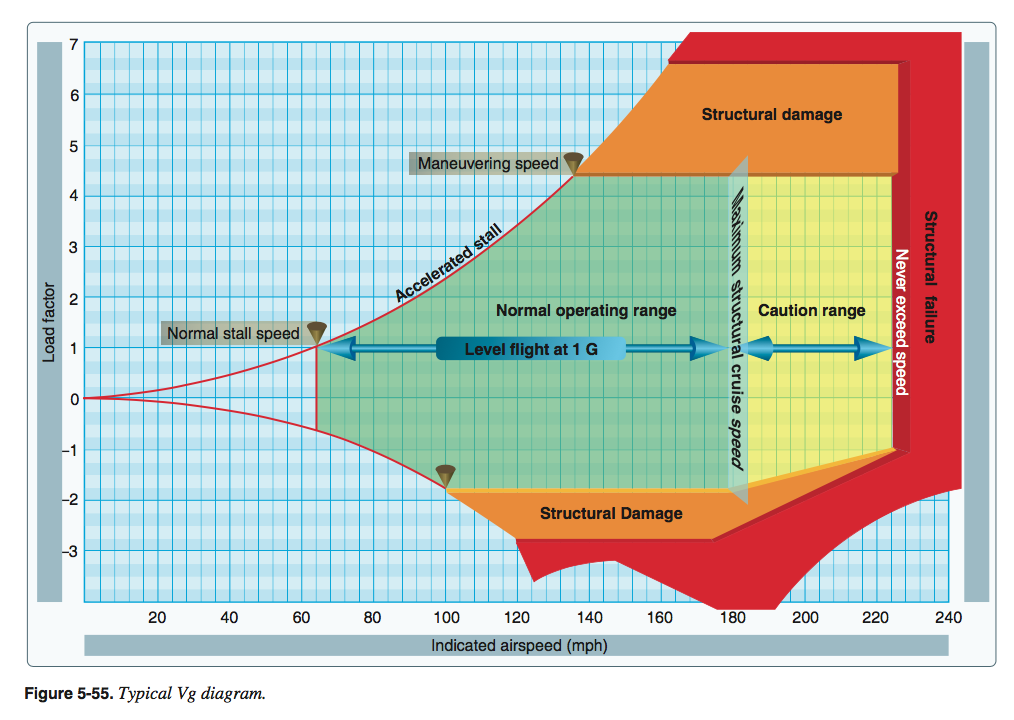
\includegraphics[width=\linewidth]{Figures/VG Diagram.png}
			\end{figure}
		\subsubsection{V-speeds}
			There are a variety of critical speeds for an aircraft:
			\begin{enumerate}
				\item $V_\text{S0}$: the stalling speed or the minimum steady flight speed in the landing configuration. In small aircraft, this is the power-off stall speed at the maximum landing weight in the landing configuration (gear and flaps down).
				\item Design maneuvering speed ($V_A$): the maximum speed at which the structural design’s limit load can be imposed (either by gusts or full deflection of the control surfaces) without causing structural damage. It is important to consider weight when referencing this speed.
				\item Landing gear operating speed ($V_{LO}$): the maximum speed for extending or retracting the landing gear if flying an aircraft with retractable landing gear.
				\item Landing gear extended speed ($V_{LE}$): the maximum speed at which an aircraft can be safely flown with the landing gear extended.
				\item Best angle-of-climb speed ($V_X$): the airspeed at which an aircraft gains the greatest amount of altitude in a given distance. It is used during a short-field takeoff to clear an obstacle.
				\item Best rate-of-climb speed ($V_Y$): the airspeed that provides the most altitude gain in a given period of time.
				\item Single-engine best rate-of-climb ($V_{YSE}$): the best rate-of-climb or minimum rate-of-sink in a light twin-engine aircraft with one engine inoperative.
				\item Minimum control speed ($V_{MC}$): the minimum flight speed at which a light, twin-engine aircraft can be satisfactorily controlled when an engine suddenly becomes inoperative and the remaining engine is at takeoff power.
				\item $V_\text{S0}$: stalling speed in the landing configuration
				\item $V_\text{FE}$: the maximum speed with the flaps extended.
				\item $V_{S1}$: the stalling speed or the minimum steady flight speed obtained in a specified configuration. For most aircraft, this is the power-off stall speed at the maximum takeoff weight in the clean configuration.
				\item $V_{N0}$: the maximum structural cruising speed. Do not exceed this speed except in smooth air.
				\item $V_{NE}$: never exceed speed. Operating above this speed is prohibited since it may result in damage or structural failure.
			\end{enumerate}
		\subsubsection{Adverse Yaw}
			Since the downward deflected aileron produces more lift as evidenced by the wing raising, it also produces more drag. This added drag causes the wing to slow down slightly. This results in the aircraft yawing toward the wing which had experienced an increase in lift (and drag). From the pilot’s perspective, the yaw is opposite the direction of the bank. The adverse yaw is a result of differential drag and the slight difference in the velocity of the left and right wings. 
			Application of the rudder is used to counteract adverse yaw. The amount of rudder control required is greatest at low airspeeds, high angles of attack, and with large aileron deflections. Like all control surfaces at lower airspeeds, the vertical stabilizer/rudder becomes less effective and magnifies the control problems associated with adverse yaw.\footnote{\href[page=153]{./phak.pdf}{PHAK: Flight Controls - Adverse Yaw}}
	\subsection{Weather}
		\subsubsection{Atmospheric Pressure}
			The unequal heating of the Earth’s surface not only modifies air density and creates circulation patterns; it also causes changes in air pressure or the force exerted by the weight of air molecules. The actual pressure at a given place and time differs with altitude, temperature, and density of the air. These conditions also affect aircraft performance, especially with regard to takeoff, rate of climb, and landings.

			\begin{enumerate}
				\item High Pressure - In the northern hemisphere, follow the right-hand-rule: sinking air, clock-wise rotation.
				\item Low Pressure - In the northern hemisphere, rising air anti-clockwise roration.
			\end{enumerate}

			High-pressure systems are generally areas of dry, descending air. Good weather is typically associated with high-pressure systems for this reason. Conversely, air flows into a low- pressure area to replace rising air. This air usually brings increasing cloudiness and precipitation. Thus, bad weather is commonly associated with areas of low pressure.

			In the lower atmosphere air generally flows perpedicular to isobars, along the pressure gradient, from regions of high pressure to low pressure. In the upper atmosphere, air generally flows parallel to isobars, perpendicular to the pressure gradient.\\

			As altitude increases, atmospheric pressure decreases. On average, with every 1,000 feet of increase in altitude, the atmospheric pressure decreases 1 "Hg. As pressure decreases, the air becomes less dense or thinner. This is the equivalent of being at a higher altitude and is referred to as density altitude. As pressure decreases, density altitude increases and has a pronounced effect on aircraft performance.

		\subsubsection{Wind}
			Air flows from areas of high pressure into areas of low pressure because air always seeks out lower pressure. The combination of atmospheric pressure differences, Coriolis force, friction, and temperature differences of the air near the earth cause two kinds of atmospheric motion: convective currents (upward and downward motion) and wind (horizontal motion). Currents and winds are important as they affect takeoff, landing, and cruise flight operations. Most importantly, currents and winds or atmospheric circulation cause weather changes.

			Convective currents are particularly noticeable in areas with a land mass directly adjacent to a large body of water, such as an ocean, large lake, or other appreciable area of water. During the day, land heats faster than water, so the air over the land becomes warmer and less dense. It rises and is replaced by cooler, denser air flowing in from over the water. This causes an onshore wind called a sea breeze. Conversely, at night land cools faster than water, as does the corresponding air. In this case, the warmer air over the water rises and is replaced by the cooler, denser air from the land, creating an offshore wind called a land breeze. This reverses the local wind circulation pattern. Convective currents can occur anywhere there is an uneven heating of the Earth’s surface. 

			\paragraph{Low-Level Wind Shear}
				Wind shear is a sudden, drastic change in wind speed and/or direction over a very small area. Wind shear can subject an aircraft to violent updrafts and downdrafts, as well as abrupt changes to the horizontal movement of the aircraft. While wind shear can occur at any altitude, low-level wind shear is especially hazardous due to the proximity of an aircraft to the ground. Low-level wind shear is commonly associated with passing frontal systems, thunderstorms, temperature inversions, and strong upper level winds (greater than 25 knots).
				The most severe type of low-level wind shear, a microburst, is associated with convective precipitation into dry air at cloud base. Microburst activity may be indicated by an intense rain shaft at the surface but virga at cloud base and a ring of blowing dust is often the only visible clue. A typical microburst has a horizontal diameter of 1–2 miles and a nominal depth of 1,000 feet. The lifespan of a microburst is about 5–15 minutes during which time it can produce downdrafts of up to 6,000 feet per minute (fpm) and headwind losses of 30–90 knots, seriously degrading performance.

		\subsubsection{Atmospheric Circulation}
			Certain factors combine to set the atmosphere in motion, but a major factor is the uneven heating of the Earth’s surface. This heating upsets the equilibrium of the atmosphere, creating changes in air movement and atmospheric pressure. The movement of air around the surface of the Earth is called atmospheric circulation. Heating of the Earth’s surface is accomplished by several processes, but in the simple convection-only model used for this discussion, the Earth is warmed by energy radiating from the sun. The process causes a circular motion that results when warm air rises and is replaced by cooler air. Warm air rises because heat causes air molecules to spread apart. As the air expands, it becomes less dense and lighter than the surrounding air. As air cools, the molecules pack together more closely, becoming denser and heavier than warm air. As a result, cool, heavy air tends to sink and replace warmer, rising air.

			In general atmospheric circulation theory, areas of low pressure exist over the equatorial regions and areas of high pressure exist over the polar regions due to a difference in temperature. The resulting low pressure allows the high pressure air at the poles to flow along the planet’s surface toward the equator. 
		\subsubsection{Atmospheric Stability}

			The stability of the atmosphere depends on its ability to resist vertical motion. A stable atmosphere makes vertical movement difficult, and small vertical disturbances dampen out and disappear. In an unstable atmosphere, small vertical air movements tend to become larger, resulting in turbulent airflow and convective activity. Instability can lead to significant turbulence, extensive vertical clouds, and severe weather. Rising air expands and cools due to the decrease in air pressure as altitude increases. The opposite is true of descending air; as atmospheric pressure increases, the temperature of descending air increases as it is compressed. Adiabatic heating and adiabatic cooling are terms used to describe this temperature change.  The rate at which temperature decreases with an increase in altitude is referred to as its lapse rate.  The dry adiabatic lapse rate (unsaturated air) is 3 $^\circ$C (5.4 $^\circ$F) per 1,000 feet. The moist adiabatic lapse rate varies from 1.1 $^\circ$C to 2.8 $^\circ$C (2 $^\circ$F to 5 $^\circ$F) per 1,000 feet.  As air ascends through the atmosphere, the average rate of temperature change is 2 $^\circ$C (3.5 $^\circ$F) per 1,000 feet.

		\subsubsection{Clouds}
			The relationship between dew point and temperature defines the concept of relative humidity. The dew point, given in degrees, is the temperature at which the air can hold no more moisture. When the temperature of the air is reduced to the dew point, the air is completely saturated and moisture begins to condense out of the air in the form of fog, dew, frost, clouds, rain, or snow. As moist, unstable air rises, clouds often form at the altitude where temperature and dew point reach the same value. When lifted, unsaturated air cools at a rate of 5.4 $^\circ$F per 1,000 feet and the dew point temperature decreases at a rate of 1 °F per 1,000 feet. This results in a convergence of temperature and dew point at a rate of 4.4 $^\circ$F. Apply the convergence rate to the reported temperature and dew point to determine the height of the cloud base.

			\begin{enumerate}
				\item Cumulus: heaped or piled clouds
				\item Stratus: layer clouds
				\item Cirrus: ringlets, fibrous clouds, also high level clouds above 20,000 feet
				\item Castellanus: common base with separate vertical development, castle-like
				\item Lenticular: lens-shaped, formed over mountains in strong winds
				\item Nimbus: rain-bearing clouds
				\item Fracto: ragged or broken
				\item Alto: middle level clouds existing at 5,000 to 20,000 feet
			\end{enumerate}
		\subsubsection{Thunderstorms}
			A thunderstorm makes its way through three distinct stages before dissipating. 
			\begin{enumerate}
				\item Cumulus stage: in which lifting action of the air begins. If sufficient moisture and instability are present, the clouds continue to increase in vertical height. Continuous, strong updrafts prohibit moisture from falling.
				\item Mature stage: Within approximately 15 minutes, the thunderstorm reaches the mature stage, which is the most violent time period of the thunderstorm’s life cycle. At this point, drops of moisture, whether rain or ice, are too heavy for the cloud to support and begin falling in the form of rain or hail. This creates a downward motion of the air. Warm, rising air; cool, precipitation-induced descending air; and violent turbulence all exist within and near the cloud. Below the cloud, the down-rushing air increases surface winds and decreases the temperature. 
				\item Dissipating stage: Once the vertical motion near the top of the cloud slows down, the top of the cloud spreads out and takes on an anvil-like shape. This is when the downdrafts spread out and replace the updrafts needed to sustain the storm. 
			\end{enumerate}	
		\subsubsection{Fog}
			\begin{enumerate}
				\item Radiation Fog: moist air is cooled by a cooler land mass to the dew point, leading to fog; typically on cool clear nights
				\item Advection Fog: warm humid air is transported over a cooler surface, which can occur near costal areas in the winter
				\item Upslope Fog: as warm moist air is driven up a mountain slope, it cools adiabatically to thr dew point
				\item Frontal fog/percipitation-induced fog: forms near a front when raindrops, falling from relatively warm air above a frontal surface, evaporate into cooler air close to the Earth’s surface and cause it to become saturated.
				\item Steam Fog: cold, dry air moves over warm water. As the water evaporates, it rises and resembles smoke. This type of fog is common over bodies of water during the coldest times of the year. Low-level turbulence and icing are commonly associated with steam fog.
				\item Ice Fog: occurs in cold weather when the temperature is much below freezing and water vapor forms directly into ice crystals. Conditions favorable for its formation are the same as for radiation fog except for cold temperature usually –25 $^\circ$F or colder.
			\end{enumerate}
		\subsubsection{Fronts}
			\begin{enumerate}
				\item \textbf{Cold Front}: A cold front occurs when a mass of cold, dense, and stable air advances and replaces a body of warmer air. Cold fronts move more rapidly than warm fronts, progressing at a rate of 25 to 30 mph. A typical cold front moves in a manner opposite that of a warm front. It is so dense, it stays close to the ground and acts like a snowplow, sliding under the warmer air and forcing the less dense air aloft. The rapidly ascending air causes the temperature to decrease suddenly, forcing the creation of clouds. The type of clouds that form depends on the stability of the warmer air mass. Prior to the passage of a typical cold front, cirriform or towering cumulus clouds are present, and cumulonimbus clouds may develop. Rain showers may also develop due to the rapid development of clouds. A high dew point and falling barometric pressure are indicative of imminent cold front passage. As the cold front passes, towering cumulus or cumulonimbus clouds continue to dominate the sky. Depending on the intensity of the cold front, heavy rain showers form and may be accompanied by lightning, thunder, and/or hail. More severe cold fronts can also produce tornadoes. During cold front passage, the visibility is poor with winds variable and gusty, and the temperature and dew point drop rapidly. A quickly falling barometric pressure bottoms out during frontal passage, then begins a gradual increase.
				\item \textbf{Warm Front}: A warm front occurs when a warm mass of air advances and replaces a body of colder air.  The slope of the advancing front slides over the top of the cooler air and gradually pushes it out of the area. Warm fronts contain warm air that often has very high humidity. As the warm air is lifted, the temperature drops and condensation occurs. Generally, prior to the passage of a warm front, cirriform or stratiform clouds, along with fog, can be expected to form along the frontal boundary. In the summer months, cumulonimbus clouds (thunderstorms) are likely to develop. During the passage of a warm front, stratiform clouds are visible and drizzle may be falling. The visibility is generally poor, but improves with variable winds. The temperature rises steadily from the inflow of relatively warmer air. For the most part, the dew point remains steady and the pressure levels off. After the passage of a warm front, stratocumulus clouds predominate and rain showers are possible.  
				\item \textbf{Occluded Front}: An occluded front occurs when a fast-moving cold front catches up with a slow-moving warm front. As the occluded front approaches, warm front weather prevails but is immediately followed by cold front weather. There are two types of occluded fronts that can occur, and the temperatures of the colliding frontal systems play a large part in defining the type of front and the resulting weather. A cold front occlusion occurs when a fast moving cold front is colder than the air ahead of the slow moving warm front. When this occurs, the cold air replaces the cool air and forces the warm front aloft into the atmosphere. Typically, the cold front occlusion creates a mixture of weather found in both warm and cold fronts, providing the air is relatively stable. A warm front occlusion occurs when the air ahead of the warm front is colder than the air of the cold front. When this is the case, the cold front rides up and over the warm front. If the air forced aloft by the warm front occlusion is unstable, the weather is more severe than the weather found in a cold front occlusion. Embedded thunderstorms, rain, and fog are likely to occur.
				\item \textbf{Stationary Front}: When the forces of two air masses are relatively equal, the boundary or front that separates them remains stationary and influences the local weather for days. This front is called a stationary front. The weather associated with a stationary front is typically a mixture that can be found in both warm and cold fronts.
			\end{enumerate}
		\subsubsection{Icing}
			Updrafts in a thunderstorm support abundant liquid water with relatively large droplet sizes. When carried above the freezing level, the water becomes supercooled. When temperature in the upward current cools to about –15 °C, much of the remaining water vapor sublimates as ice crystals. Above this level, at lower temperatures, the amount of supercooled water decreases. Supercooled water freezes on impact with an aircraft. Clear icing can occur at any altitude above the freezing level, but at high levels, icing from smaller droplets may be rime or mixed rime and clear ice. The abundance of large, supercooled water droplets makes clear icing very rapid between 0 °C and –15 °C and encounters can be frequent in a cluster of cells. Thunderstorm icing can be extremely hazardous.
%done
\newpage
\section{Airplane Construction, Instruments, Engines, \& Controls}
	\subsection{Airplane Construction}
		\subsubsection{Fuselage}
			The fuselage is the central body of an airplane and is designed to accommodate the crew, passengers, and cargo. It also provides the structural connection for the wings and tail assembly.\footnote{\href[page=76]{./phak.pdf}{PHAK: Aircraft Construction - Fuselage}}
		\subsubsection{Wings}
			The wings are airfoils attached to each side of the fuselage and are the main lifting surfaces that support the airplane in flight. Wings may be attached at the top, middle, or lower portion of the fuselage. These designs are referred to as high-, mid-, and low-wing, respectively. In most modern airplanes, the fuel tanks are either an integral part of the wing’s structure or consist of flexible containers mounted inside of the wing.\footnote{\href[page=76]{./phak.pdf}{PHAK: Aircraft Construction - Wing}}
		\subsubsection{Empennage}
			The empennage includes the entire tail group and consists of fixed surfaces, such as the vertical stabilizer and the horizontal stabilizer. The movable surfaces include the rudder, the elevator, and one or more trim tabs.\footnote{\href[page=79]{./phak.pdf}{PHAK: Aircraft Construction - Empennage}}
		\subsubsection{Engine/Powerplant}
			The powerplant usually includes both the engine and the propeller. The primary function of the engine is to provide the power to turn the propeller. It also generates electrical power, provides a vacuum source for some flight instruments, and in most single-engine airplanes, provides a source of heat for the pilot and passengers. The propeller, mounted on the front of the engine, translates the rotating force of the engine into thrust, a forward acting force that helps move the airplane through the air. A propeller is a rotating airfoil that produces thrust through aerodynamic action. A high-pressure area is formed at the back of the propeller’s airfoil, and low pressure is produced at the face of the propeller, similar to the way lift is generated by an airfoil used as a lifting surface or wing. This pressure differential develops thrust from the propeller, which in turn pulls the airplane forward. Engines may be turned around to be pushers with the propeller at the rear.\footnote{\href[page=80]{./phak.pdf}{PHAK: Aircraft Construction - The Powerplant}}
		\subsubsection{Landing Gear}
			The landing gear is the principal support of the airplane when parked, taxiing, taking off, or landing. The most common type of landing gear consists of wheels, but airplanes can also be equipped with floats for water operations or skis for landing on snow. \footnote{\href[page=80]{./phak.pdf}{PHAK: Aircraft Construction - Landing Gear}}
	\subsection{Engine/Powerplant}
		\subsubsection{Reciprocating (Piston) Engines}
			The two primary reciprocating engine designs are the spark ignition and the compression ignition. They are directly comparable to a automobile gasoline engine and a diesel engine respectively. The main difference between spark ignition and compression ignition is the process of igniting the fuel. Spark ignition engines use a spark plug to ignite a pre-mixed fuel-air mixture. A compression ignition engine compresses the air in the cylinder, raising its temperature to a degree necessary for automatic ignition when fuel is injected into the cylinder.\footnote{\href[page=164]{./phak.pdf}{PHAK: Aircraft Systems - Reciprocating Engines}}\\
			The two engine designs are further classified:
				\begin{enumerate}
					\item Cylinder arrangement w.r.t the crankshaft; radial, in-line, v-type, or opposed
					\item Operating cycle: two or four stroke
						\begin{itemize}
							\item In a two-stroke engine, the conversion of chemical energy into mechanical energy occurs over a two-stroke operating cycle. The intake, compression, power, and exhaust processes occur in only two strokes of the piston rather than the more common four strokes.
							\item In a four-stroke engine, the conversion of chemical energy into mechanical energy occurs over a four-stroke operating cycle. The intake, compression, power, and exhaust processes occur in four separate strokes of the piston.
						\end{itemize}
					\item Method of cooling: liquid or air
				\end{enumerate}
		\subsubsection{Propeller Types}
			The propeller is used to convert the rotation of the engine's crankshaft into thrust. The propeller itself is twisted so the blade angle changes from hub to tip. The greatest angle of incidence, or the highest pitch, is at the hub while the smallest angle of incidence or smallest pitch is at the tip. The reason for the twist is to produce uniform lift from the hub to the tip. As the blade rotates, there is a difference in the actual speed of the various portions of the blade. The tip of the blade travels faster than the part near the hub, because the tip travels a greater distance than the hub in the same length of time.\footnote{\href[page=166]{./phak.pdf}{PHAK: Aircraft Systems - The Propeller}}
			\paragraph{Fixed-Pitch Propeller}
				A propeller with fixed blade angles is a fixed-pitch propeller. The pitch of this propeller is set by the manufacturer and cannot be changed. In this case, the rpm of the propeller would be the same as the crankshaft rpm. In a fixed-pitch propeller, the tachometer is the indicator of engine power. A tachometer is calibrated in hundreds of rpm and gives a direct indication of the engine and propeller rpm. When operating altitude increases, the tachometer may not show correct power output of the engine. For example, 2,300 rpm at 5,000 feet produces less horsepower than 2,300 rpm at sea level because power output depends on air density. As altitude is increased, the throttle must be opened further to indicate the same rpm as at a lower altitude.\footnote{\href[page=166]{./phak.pdf}{PHAK: Aircraft Systems - Fixed Pitch Propeller}}
			\paragraph{Variable-Pitch/Constant-Speed Propeller}
				A constant-speed propeller is a controllable-pitch propeller whose pitch is automatically varied in flight by a governor maintaining constant rpm despite varying air loads. It is the most common type of adjustable-pitch propeller. The main advantage of a constant-speed propeller is that it converts a high percentage of brake horsepower (BHP) into thrust horsepower (THP) over a wide range of rpm and airspeed combinations. A constant-speed propeller is more efficient than other propellers because it allows selection of the most efficient engine rpm for the given conditions. Once a specific rpm is selected, a governor automatically adjusts the propeller blade angle as necessary to maintain the selected rpm. For example, after setting the desired rpm during cruising flight, an increase in airspeed or decrease in propeller load causes the propeller blade angle to increase as necessary to maintain the selected rpm. A reduction in airspeed or increase in propeller load causes the propeller blade angle to decrease. On aircraft equipped with a constant-speed propeller, power output is controlled by the throttle and indicated by a manifold pressure gauge.\footnote{\href[page=168]{./phak.pdf}{PHAK: Aircraft Systems - Adjustable Pitch Propeller}}\\
				When both manifold pressure and rpm need to be changed, avoid engine overstress by making power adjustments in the proper order:
					\begin{itemize}
						\item When power settings are being decreased, reduce manifold pressure before reducing rpm. If rpm is reduced before manifold pressure, manifold pressure automatically increases, possibly exceeding the manufacturer’s tolerances.
						\item When power settings are being increased, reverse the order—increase rpm first, then manifold pressure.
						\item To prevent damage to radial engines, minimize operating time at maximum rpm and manifold pressure, and avoid operation at maximum rpm and low manifold pressure.
					\end{itemize}
		\subsubsection{Carburetor}
			Float-type carburetors, complete with idling, accelerating, mixture control, idle cutoff, and power enrichment systems, are the most common of the two carburetor types. In the operation of the float-type carburetor system, the outside air first flows through an air filter, usually located at an air intake in the front part of the engine cowling. This filtered air flows into the carburetor and through a venturi, a narrow throat in the carburetor. When the air flows through the venturi, a low-pressure area is created that forces the fuel to flow through a main fuel jet located at the throat. The fuel then flows into the airstream where it is mixed with the flowing air. 
			The fuel-air mixture is then drawn through the intake manifold and into the combustion chambers where it is ignited. The chief disadvantage of the float-type carburetor, however, is its icing tendency. Since the float-type carburetor must discharge fuel at a point of low pressure, the discharge nozzle must be located at the venturi throat, and the throttle valve must be on the engine side of the discharge nozzle. This means that the drop in temperature due to fuel vaporization takes place within the venturi. As a result, ice readily forms in the venturi and on the throttle valve.\footnote{\href[page=170]{./phak.pdf}{PHAK: Aircraft Systems - Carburetor Systems}}
		\subsubsection{Fuel Injection}
			In a fuel injection system, the fuel is injected directly into the cylinders, or just ahead of the intake valve. The air intake for the fuel injection system is similar to that used in a carburetor system, with an alternate air source located within the engine cowling. This source is used if the external air source is obstructed. The alternate air source is usually operated automatically, with a backup manual system that can be used if the automatic feature malfunctions. A fuel injection system usually incorporates six basic components: an engine-driven fuel pump, a fuel-air control unit, a fuel manifold (fuel distributor), discharge nozzles, an auxiliary fuel pump, and fuel pressure/flow indicators.\footnote{\href[page=173]{./phak.pdf}{PHAK: Aircraft Systems - Fuel Injection Systems}}
		\subsubsection{Ignition System}
		%todo
		\subsubsection{Oil Systems}
		%todo
		\subsubsection{Engine Cooling Systems}
		%todo
	\subsection{Airframe Systems}
		\subsubsection{Fuel Systems}
			The fuel system is designed to provide an uninterrupted flow of clean fuel from the fuel tanks to the engine. The fuel must be available to the engine under all conditions of engine power, altitude, attitude, and during all approved flight maneuvers. Two common classifications apply to fuel systems in small aircraft: gravity­-feed and fuel-­pump systems.\footnote{\href[page=187]{./phak.pdf}{PHAK: Aircraft Systems - Fuel Systems}}
			\begin{itemize}
				\item Gravity-Feed System: The gravity­-feed system utilizes the force of gravity to transfer the fuel from the tanks to the engine.
				\item Fuel-Pump System: Aircraft with fuel­pump systems have two fuel pumps. The main pump system is engine driven with an electrically­ driven auxiliary pump provided for use in engine starting and in the event the engine pump fails. The auxiliary pump, also known as a boost pump, provides added reliability to the fuel system. 
			\end{itemize}
			The fuel selector valve allows selection of fuel from various tanks. A common type of selector valve contains four positions: LEFT, RIGHT, BOTH, and OFF. Selecting the LEFT or RIGHT position allows fuel to feed only from the respective tank, while selecting the BOTH position feeds fuel from both tanks. The LEFT or RIGHT position may be used to balance the amount of fuel remaining in each wing tank. 
		\subsubsection{Hydraulic Systems}
		\subsubsection{Alternator/Battery}
			Alternators produce sufficient current to operate the entire electrical system, even at slower engine speeds, by producing alternating current (AC), which is converted to DC. The electrical output of an alternator is more constant throughout a wide range of engine speeds. A voltage regulator controls the rate of charge to the battery by stabilizing the generator or alternator electrical output. The generator/alternator voltage output should be higher than the battery voltage. For example, a 12-volt battery would be fed by a generator/alternator system of approximately 14 volts. The difference in voltage keeps the battery charged. \footnote{\href[page=192]{./phak.pdf}{PHAK: Aircraft Systems - Electrical System}}
	\subsection{Flight Controls}
		\subsubsection{Primary Flight Controls}
			\paragraph{Aileron}
				Ailerons control roll about the longitudinal axis. The ailerons are attached to the outboard trailing edge of each wing and move in the opposite direction from each other. Ailerons are connected by cables, bellcranks, pulleys, and/or push-pull tubes to a control wheel or control stick. Moving the control wheel, or control stick, to the right causes the right aileron to deflect upward and the left aileron to deflect downward. The upward deflection of the right aileron decreases the camber resulting in decreased lift on the right wing. The corresponding downward deflection of the left aileron increases the camber resulting in increased lift on the left wing. Thus, the increased lift on the left wing and the decreased lift on the right wing causes the aircraft to roll to the right.\footnote{\href[page=153]{./phak.pdf}{PHAK: Flight Controls - Ailerons}}
			\paragraph{Rudder}
				The rudder controls movement of the aircraft about its vertical axis. This motion is called yaw. Like the other primary control surfaces, the rudder is a movable surface hinged to a fixed surface in this case, to the vertical stabilizer or fin. The rudder is controlled by the left and right rudder pedals. When the rudder is deflected into the airflow, a horizontal force is exerted in the opposite direction. By pushing the left pedal, the rudder moves left. This alters the airflow around the vertical stabilizer/rudder and creates a horizontal component of lift that moves the tail to the right and yaws the nose of the airplane to the left. \footnote{\href[page=158]{./phak.pdf}{PHAK: Flight Controls - Rudder}}
			\paragraph{Elevator}
				The elevator controls pitch about the lateral axis. Like the ailerons on small aircraft, the elevator is connected to the control column in the flight deck by a series of mechanical linkages. The up-elevator position decreases the camber of the elevator and creates a downward aerodynamic force, which is greater than the normal tail-down force that exists in straight-and­ level flight. The overall effect causes the tail of the aircraft to move down and the nose to pitch up. The torque applied by the pitching moment is determined by the distance between the CG and the horizontal tail surface, as well as by the aerodynamic effectiveness of the horizontal tail surface.\footnote{\href[page=155]{./phak.pdf}{PHAK: Flight Controls - Elevator}}
		\subsubsection{Secondary Flight Controls}
			\paragraph{Flaps}
				Flaps are the most common high-lift devices used on aircraft. These surfaces, which are attached to the trailing edge of the wing, increase both lift and induced drag for any given AOA. Flaps allow a compromise between high cruising speed and low landing speed because they may be extended when needed and retracted into the wing’s structure when not needed. \footnote{\href[page=158]{./phak.pdf}{PHAK: Flight Controls - Flaps}}
			\paragraph{Leading Edge Devices}
				High-lift devices also can be applied to the leading edge of the airfoil. The most common types are fixed slots, movable slats, leading edge flaps, and cuffs. Fixed slots direct airflow to the upper wing surface and delay airflow separation at higher angles of attack. Movable slats consist of leading edge segments that move on tracks. At low angles of attack, each slat is held flush against the wing’s leading edge by the high pressure that forms at the wing’s leading edge. As the AOA increases, the high- pressure area moves aft below the lower surface of the wing, allowing the slats to move forward. Opening a slat allows the air below the wing to flow over the wing’s upper surface, delaying airflow separation. Leading edge flaps, like trailing edge flaps, are used to increase both CL-MAX and the camber of the wings. Leading edge cuffs, like leading edge flaps and trailing edge flaps are used to increase both CL-MAX and the camber of the wings. Unlike leading edge flaps and trailing edge flaps, leading edge cuffs are fixed aerodynamic devices. In most cases, leading edge cuffs extend the leading edge down and forward. This causes the airflow to attach better to the upper surface of the wing at higher angles of attack, thus lowering an aircraft’s stall speed. \footnote{\href[page=159]{./phak.pdf}{PHAK: Flight Controls - Leading Edge Devices}}
			\paragraph{Spoilers}
				Found on some fixed-wing aircraft, high drag devices called spoilers are deployed from the wings to spoil the smooth airflow, reducing lift and increasing drag.  On other aircraft, spoilers are often used for roll control, an advantage of which is the elimination of adverse yaw.\footnote{\href[page=160]{./phak.pdf}{PHAK: Flight Controls - Spoilers}}
			\paragraph{Trim}
				Trim systems are used to relieve the pilot of the need to maintain constant pressure on the flight controls, and usually consist of flight deck controls and small hinged devices attached to the trailing edge of one or more of the primary flight control surfaces. Designed to help minimize a pilot’s workload, trim systems aerodynamically assist movement and position of the flight control surface to which they are attached. Common types of trim systems include trim tabs, balance tabs, antiservo tabs, ground adjustable tabs, and an adjustable stabilizer.\footnote{\href[page=160]{./phak.pdf}{PHAK: Flight Controls - Trim Systems}}
		\subsection{Engine Controls}
			\subsubsection{Throttle \& Mixture}
				The engine rpm is regulated by the throttle, which controls the fuel-air flow to the engine. The mixture control only controls the amount of fuel, independent of the amount of air. The reason this control exists is that as altitude increases, the density of air entering the carburetor decreases, while the density of the fuel remains the same. This creates a progressively richer mixture that can result in engine roughness and an appreciable loss of power. The roughness normally is due to spark plug fouling from excessive carbon buildup on the plugs. Carbon buildup occurs because the rich mixture lowers the temperature inside the cylinder, inhibiting complete combustion of the fuel. During a descent from high altitude, the fuel-air mixture must be enriched, or it may become too lean. An overly lean mixture causes detonation, which may result in rough engine operation, overheating, and/or a loss of power.\footnote{\href[page=171]{./phak.pdf}{PHAK: Aircraft Systems - Mixture Control}} 
			\subsubsection{Carburetor Heat}
				Carburetor heat is an anti-icing system that preheats the air before it reaches the carburetor and is intended to keep the fuel-air mixture above freezing to prevent the formation of carburetor ice. Carburetor heat can be used to melt ice that has already formed in the carburetor if the accumulation is not too great, but using carburetor heat as a preventative measure is the better option. The use of carburetor heat causes a decrease in engine power, sometimes up to 15 percent, because the heated air is less dense than the outside air that had been entering the engine. This enriches the mixture. When ice is present in an aircraft with a fixed-pitch propeller and carburetor heat is being used, there is a decrease in rpm, followed by a gradual increase in rpm as the ice melts. The engine also should run more smoothly after the ice has been removed. If ice is not present, the rpm decreases and then remains constant. When carburetor heat is used on an aircraft with a constant-speed propeller and ice is present, a decrease in the manifold pressure is noticed, followed by a gradual increase. If carburetor icing is not present, the gradual increase in manifold pressure is not apparent until the carburetor heat is turned off.\footnote{\href[page=172]{./phak.pdf}{PHAK: Aircraft Systems - Carburetor Heat}}
			\subsubsection{Propeller}
				Whereas the throttle controls power output, and the propeller control regulates engine rpm. This regulates propeller rpm, which is registered on the tachometer. A propeller control varies from fine to coarse pitch (alternatively, low to high blade angle of attack) Once the rpm settings for the propeller are selected, the propeller governor automatically adjusts the blade angle to maintain the selected rpm. It does this by using oil pressure. Generally, the oil pressure used for pitch change comes directly from the engine lubricating system.\footnote{\href[page=197]{./afh.pdf}{AFH: Transition to Complex Airplanes - Blade Angle Control}}\\

				\begin{figure}[H]
					\centering
					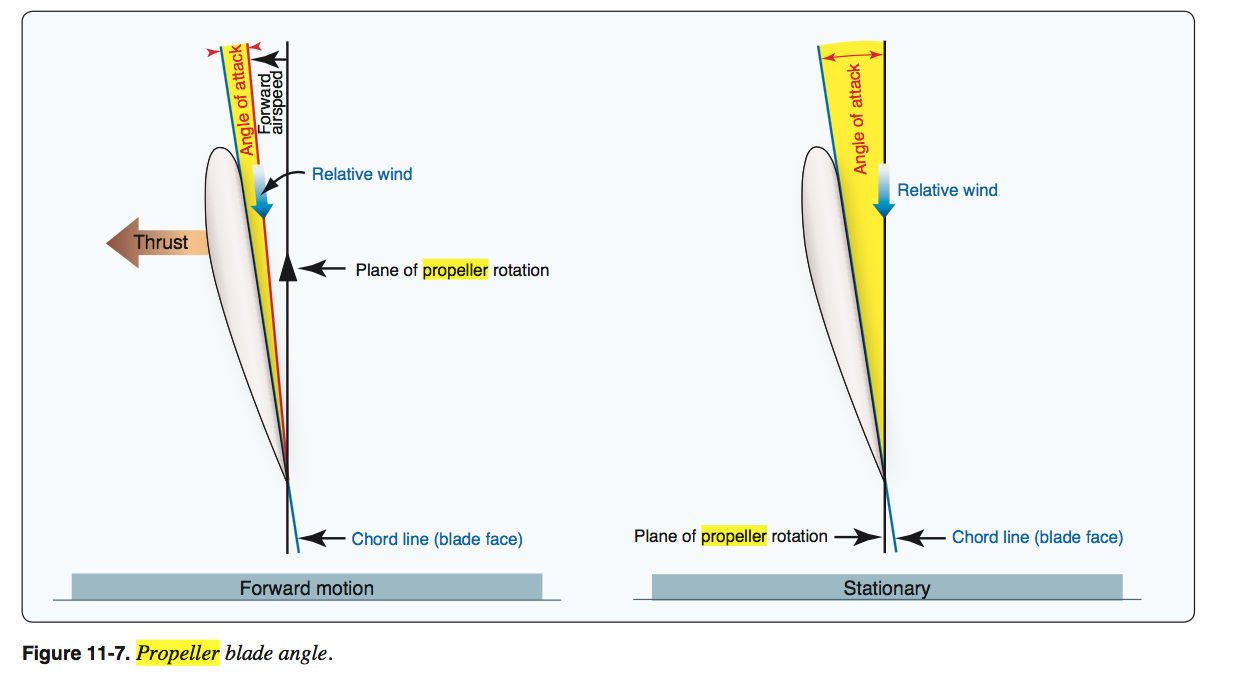
\includegraphics[width=0.8\linewidth]{Figures/Propeller Blade Control.png}
				\end{figure}

				During takeoff, when the forward motion of the airplane is at low speeds and when maximum power and thrust are required, the constant-speed propeller sets up a low propeller blade angle (pitch). The low blade angle keeps the AOA, with respect to the relative wind, small and efficient at the low speed. At the same time, it allows the propeller to handle a smaller mass of air per revolution. This light load allows the engine to turn at maximum rpm and develop maximum power. Although the mass of air per revolution is small, the number of rpm is high. For climb after takeoff, the power output of the engine is reduced to climb power by decreasing the manifold pressure and lowering rpm by increasing the blade angle. At the higher (climb) airspeed and the higher blade angle, the propeller is handling a greater mass of air per second at a lower slipstream velocity. This reduction in power is offset by the increase in propeller efficiency. The AOA is again kept small by the increase in the blade angle with an increase in airspeed.\footnote{\href[page=194]{./afh.pdf}{AFH: Transition to Complex Airplanes - Controllable-Pitch Propeller, Takeoff, Climb, and Cruise}}

				On some constant-speed propellers, changes in pitch are obtained by the use of an inherent centrifugal twisting moment of the blades that tends to flatten the blades toward low pitch and oil pressure applied to a hydraulic piston connected to the propeller blades which moves them toward high pitch. Another type of constant-speed propeller uses counterweights attached to the blade shanks in the hub. Governor oil pressure and the blade twisting moment move the blades toward the low pitch position, and centrifugal force acting on the counterweights moves them (and the blades) toward the high pitch position. In the first case above, governor oil pressure moves the blades towards high pitch and in the second case, governor oil pressure and the blade twisting moment move the blades toward low pitch. A loss of governor oil pressure, therefore, affects each differently.\footnote{\href[page=197]{./afh.pdf}{AFH: Transition to Complex Airplanes - Blade Angle Control}}

			\subsubsection{Ignition System}
				In a spark ignition engine, the ignition system provides a spark that ignites the fuel-air mixture in the cylinders and is made up of magnetos, spark plugs, high-tension leads, and an ignition switch. A magneto uses a permanent magnet to generate an electrical current completely independent of the aircraft’s electrical system. The magneto generates sufficiently high voltage to jump a spark across the spark plug gap in each cylinder. The system begins to fire when the starter is engaged and the crankshaft begins to turn. It continues to operate whenever the crankshaft is rotating. Most standard certificated aircraft incorporate a dual ignition system with two individual magnetos, separate sets of wires, and spark plugs to increase reliability of the ignition system. Each magneto operates independently to fire one of the two spark plugs in each cylinder. The firing of two spark plugs improves combustion of the fuel-air mixture and results in a slightly higher power output. If one of the magnetos fails, the other is unaffected. The engine continues to operate normally, although a slight decrease in engine power can be expected. The same is true if one of the two spark plugs in a cylinder fails.\\
				The operation of the magneto is controlled in the flight deck by the ignition switch. The switch has five positions:
					\begin{enumerate}
						\item OFF - grounds both magnetos
						\item R (right) - only right magneto
						\item L (left) - only left magneto 
						\item BOTH - both magnetos
						\item START - both magnetos, and engage starter motor
					\end{enumerate}
				A malfunctioning ignition system can be identified during the pretakeoff check by observing the decrease in rpm that occurs when the ignition switch is first moved from BOTH to RIGHT and then from BOTH to LEFT. A small decrease in engine rpm is normal during this check. The permissible decrease is listed in the AFM or POH. If the engine stops running when switched to one magneto or if the rpm drop exceeds the allowable limit, do not fly the aircraft until the problem is corrected. The cause could be fouled plugs, broken or shorted wires between the magneto and the plugs, or improperly timed firing of the plugs. It should be noted that “no drop” in rpm is not normal, and in that instance, the aircraft should not be flown. Even with the ignition switch in the OFF position, if the ground wire between the magneto and the ignition switch becomes disconnected or broken, the engine could accidentally start if the propeller is moved with residual fuel in the cylinder.\footnote{\href[page=177]{./phak.pdf}{PHAK: Aircraft Systems - Ignition System}}
			\subsubsection{Fuel System}
				The fuel system is designed to provide an uninterrupted flow of clean fuel from the fuel tanks to the engine. The fuel must be available to the engine under all conditions of engine power, altitude, attitude, and during all approved flight maneuvers. Two common classifications apply to fuel systems in small aircraft: gravity-feed and fuel-pump systems. The fuel quantity gauges indicate the amount of fuel measured by a sensing unit in each fuel tank and is displayed in gallons or pounds. Aircraft certification rules require accuracy in fuel gauges only when they read empty. The fuel selector valve allows selection of fuel from various tanks. A common type of selector valve contains four positions: LEFT, RIGHT, BOTH, and OFF. Selecting the LEFT or RIGHT position allows fuel to feed only from the respective tank, while selecting the BOTH position feeds fuel from both tanks. The LEFT or RIGHT position may be used to balance the amount of fuel remaining in each wing tank. The fuel strainer should be drained before each flight. Fuel samples should be drained and checked visually for water and contaminants. Water in the sump is hazardous because in cold weather the water can freeze and block fuel lines. In warm weather, it can flow into the carburetor and stop the engine. If water is present in the sump, more water in the fuel tanks is probable, and they should be drained until there is no evidence of water.\footnote{\href[page=187]{./phak.pdf}{PHAK: Aircraft Systems - Fuel Systems}}
	\subsection{Flight Instruments}
		\subsubsection{Pitot-Static Instruments}
			\begin{figure}[H]
				\centering
				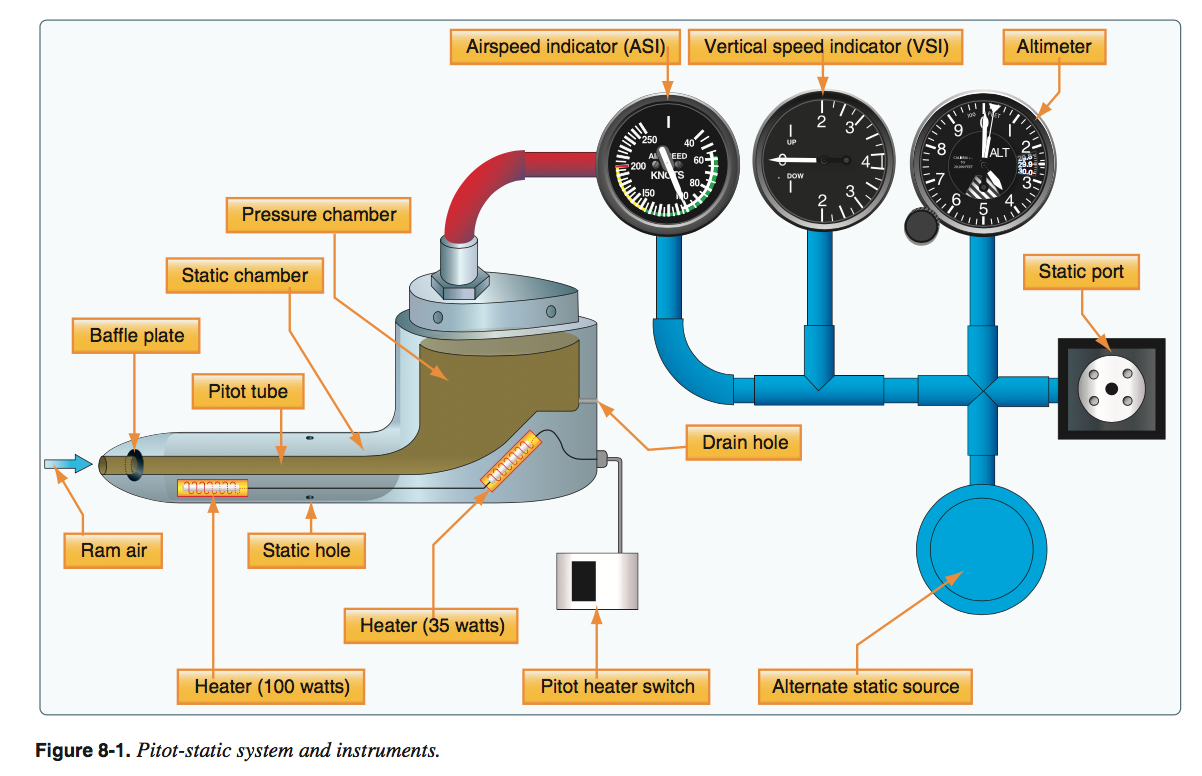
\includegraphics[width=0.8\linewidth]{Figures/Pitot-Static.png}
			\end{figure}
			\paragraph{Altimeter}
				An altimeter is essentially a barometer.It measures the height of an aircraft above a given reference pressure level. A stack of sealed aneroid wafers comprise the main component of the altimeter. An aneroid wafer is a sealed wafer that is evacuated to an internal pressure of 29.92 in Hg. These wafers are free to expand and contract with changes to the static pressure.  A mechanical linkage connects the wafer movement to the needles on the indicator face, which translates compression of the wafers into a decrease in altitude and translates an expansion of the wafers into an increase in altitude. 
				\begin{figure}[H]
					\centering
					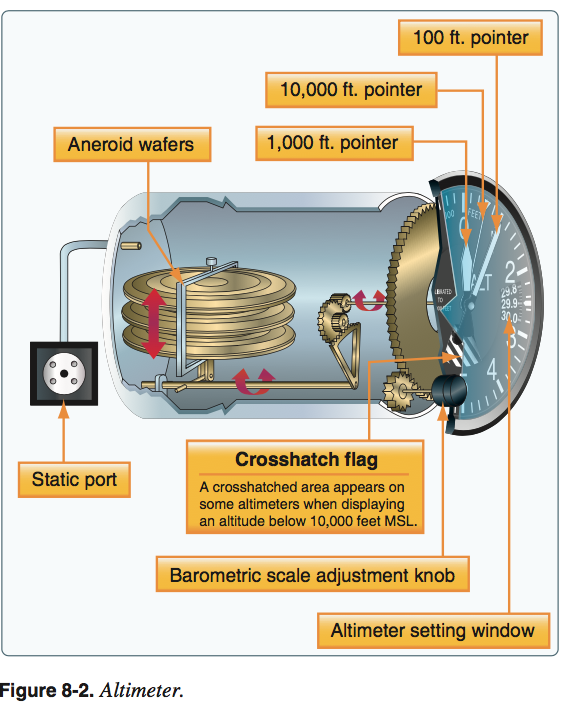
\includegraphics[width=0.5\linewidth]{Figures/Altimeter.png}
				\end{figure}
				This indicated altitude is correct, however, only when the sea level barometric pressure is standard (29.92 in Hg), the sea level free air temperature is standard ($15^\circ$C), and the pressure and temperature decrease at a standard rate with an increase in altitude.\footnote{\href[page=207]{./phak.pdf}{PHAK: Flight Instruments - Altimeter}}\\
				Errors:
					\begin{enumerate}
						\item  When moving from an area of high pressure to low pressure, the iso surfaces in the atmosphere will space further apart, leading to a reading altitude lower than true altitude. The converse is true when moving from an area of low pressure to high pressure.
						\item If the static port became blocked, the altimeter would give a stationary reading
					\end{enumerate}
			\paragraph{Airspeed Indicator}
				An airspeed indicator measures the difference between ram-air pressure and static air pressure to output a value of airspeed. These two pressures are equal when the aircraft is parked on the ground in calm air. When the aircraft moves through the air, the pressure on the pitot line becomes greater than the pressure in the static lines. This difference in pressure is registered by the airspeed pointer on the face of the instrument, which is calibrated in miles per hour, knots (nautical miles per hour), or both. The reading provides a value for indicated airspeed (more or less equivalent to calibrated airspeed).\footnote{\href[page=212]{./phak.pdf}{PHAK: Flight Instruments - Airspeed Indicator (ASI)}}\\
				Errors:
					\begin{enumerate}
						\item In ground effect, airspeed indicators can read erroneously as high pressure accumulates beneath the wing
						\item At high angles of attack airflow around the static port can become disturbed as air separates from the fuselage
						\item If the static port is blocked, the ASI continues to operate; however, it is inaccurate. The airspeed indicates lower than the actual airspeed when the aircraft is operated above the altitude where the static ports became blocked because the trapped static pressure is higher than normal for that altitude. When operating at a lower altitude, a faster than actual airspeed is displayed due to the relatively low static pressure trapped in the system.
					\end{enumerate}
				\begin{figure}[H]
					\centering
					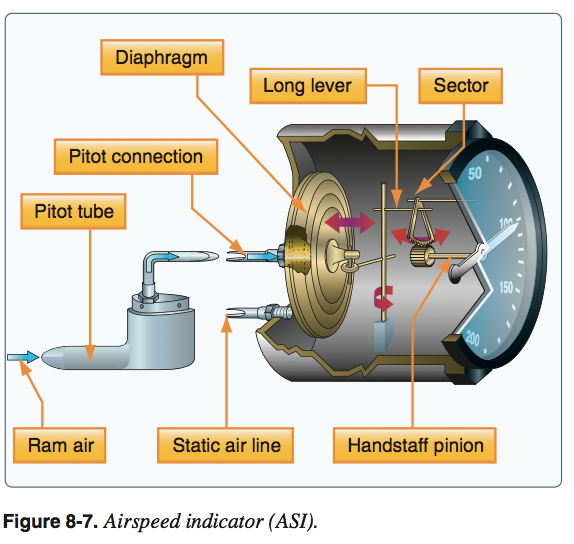
\includegraphics[width=0.5\linewidth]{Figures/Airspeed.png}
				\end{figure}
				An airspeed indicator has various color-coded markings:
					\begin{enumerate}
						\item White arc - commonly referred to as the flap operating range since its lower limit represents the full flap stall speed and its upper limit provides the maximum flap speed.
						\item Lower limit of white arc ($V_\text{S0}$) - stalling speed in the landing configuration
						\item Upper limit of the white arc ($V_\text{FE}$)—the maximum speed with the flaps extended.
						\item Green arc - the normal operating range of the aircraft. Most flying occurs within this range
						\item Lower limit of green arc ($V_{S1}$)—the stalling speed or the minimum steady flight speed obtained in a specified configuration. For most aircraft, this is the power-off stall speed at the maximum takeoff weight in the clean configuration.
						\item Upper limit of green arc ($V_{N0}$)—the maximum structural cruising speed. Do not exceed this speed except in smooth air.
						\item Yellow arc—caution range. Fly within this range only in smooth air and then only with caution.
						\item Red line ($V_{NE}$)—never exceed speed. Operating above this speed is prohibited since it may result in damage or structural failure.
					\end{enumerate}
				An aircraft has other airspeed limitations that are not marked on the face of the airspeed indicator:
					\begin{multicols}{2}
					\begin{enumerate}
						\item Design maneuvering speed ($V_A$)
						\item Landing gear operating speed ($V_{LO}$)
						\item Landing gear extended speed ($V_{LE}$)
						\item Best angle-of-climb speed ($V_X$)
						\item Best rate-of-climb speed ($V_Y$)
						\item Single-engine best rate-of-climb ($V_{YSE}$)
						\item Minimum control speed ($V_{MC}$)
					\end{enumerate}
					\end{multicols}
			\paragraph{Vertical Speed Indicator}
				\begin{figure}[H]
					\centering
					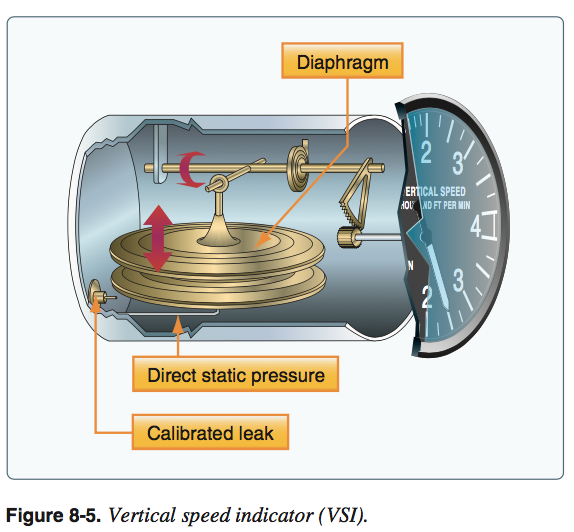
\includegraphics[width=0.5\linewidth]{Figures/VSI.png}
				\end{figure}
				A vertical speed indicator, or VSI, indicates an aircraft's rate of climb. The VSI contains a diaphragm with a calibrated leak. At a given altitude the diaphragm pressure equilibrates with the ambient air pressure. As the aircraft climbs or descends, the diaphragm and calibrated leak act as a ``memory'' of the past altitude of the aircraft. The calibrated leak allows for the direction and magnitude of the flow of air in or out of the diaphragm, which translates to a climb or descent rate.\\
				Errors:
					\begin{enumerate}
						\item If the static port is blocked, the VSI will read constant or zero
					\end{enumerate}
		\subsubsection{Gyroscopic Instruments}
			\paragraph{Attitude Indicator}
				The attitude indicator, with its miniature aircraft and horizon bar, displays a picture of the attitude of the aircraft. The relationship of the miniature aircraft to the horizon bar is the same as the relationship of the real aircraft to the actual horizon.
				\begin{figure}[H]
					\centering
					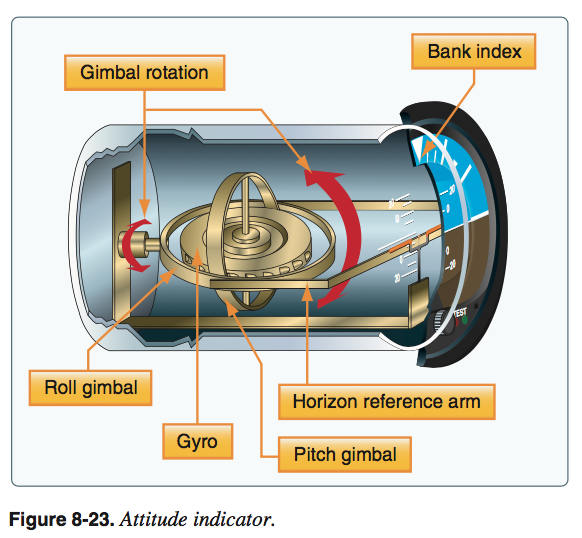
\includegraphics[width=0.5\linewidth]{Figures/Attitude.png}
				\end{figure}
				The instrument gives an instantaneous indication of even the smallest changes in attitude. The gyro in the attitude indicator is mounted in a horizontal plane and depends upon rigidity in space for its operation. The horizon bar represents the true horizon. This bar is fixed to the gyro and remains in a horizontal plane as the aircraft is pitched or banked about its lateral or longitudinal axis, indicating the attitude of the aircraft relative to the true horizon.\footnote{\href[page=222]{./phak.pdf}{PHAK: Flight Instruments - Attitude Indicator}}
			\paragraph{Turn Coordinator \& Inclinometer}
				The gimbal in the turn coordinator is canted; therefore, its gyro can sense both rate of roll and rate of turn. Since turn coordinators are more prevalent in training aircraft, this discussion concentrates on that instrument. When rolling into or out of a turn, the miniature aircraft banks in the direction the aircraft is rolled. A rapid roll rate causes the miniature aircraft to bank more steeply than a slow roll rate. The turn coordinator can be used to establish and maintain a standard-rate turn by aligning the wing of the miniature aircraft with the turn index. The inclinometer is used to depict aircraft yaw, which is the side-to-side movement of the aircraft’s nose. During coordinated, straight-and-level flight, the force of gravity causes the ball to rest in the lowest part of the tube, centered between the reference lines. Coordinated flight is maintained by keeping the ball centered. If the ball is not centered, it can be centered by using the rudder.\footnote{\href[page=221]{./phak.pdf}{PHAK: Flight Instruments - Turn Coordinator}}
				\begin{figure}[H]
					\centering
					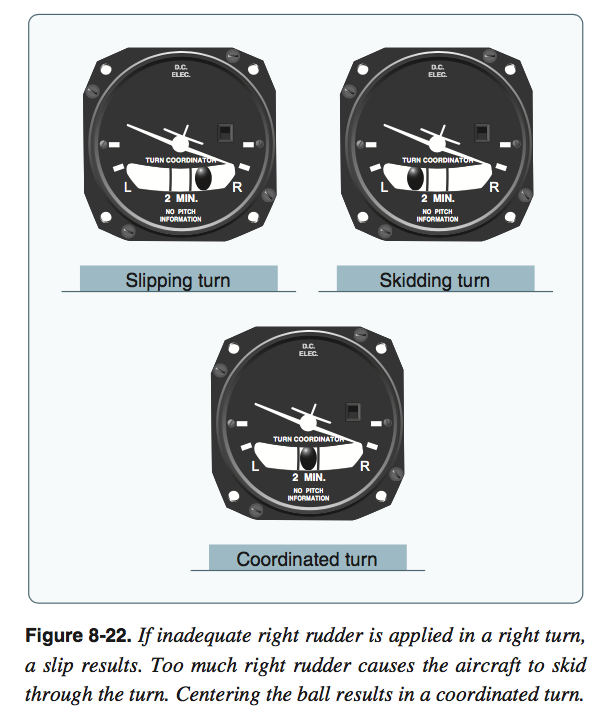
\includegraphics[width=0.5\linewidth]{Figures/Turn Coordinator.png}
				\end{figure}
			\paragraph{Heading Indicator}
				The heading indicator is fundamentally a mechanical instrument designed to facilitate the use of the magnetic compass. The operation of the heading indicator depends upon the principle of rigidity in space. The rotor turns in a vertical plane and fixed to the rotor is a compass card. Since the rotor remains rigid in space, the points on the card hold the same position in space relative to the vertical plane of the gyro. The aircraft actually rotates around the rotating gyro, not the other way around. As the instrument case and the aircraft revolve around the vertical axis of the gyro, the card provides clear and accurate heading information.\footnote{\href[page=223]{./phak.pdf}{PHAK: Flight Instruments - Heading Indicator}}
				\begin{figure}[H]
					\centering
					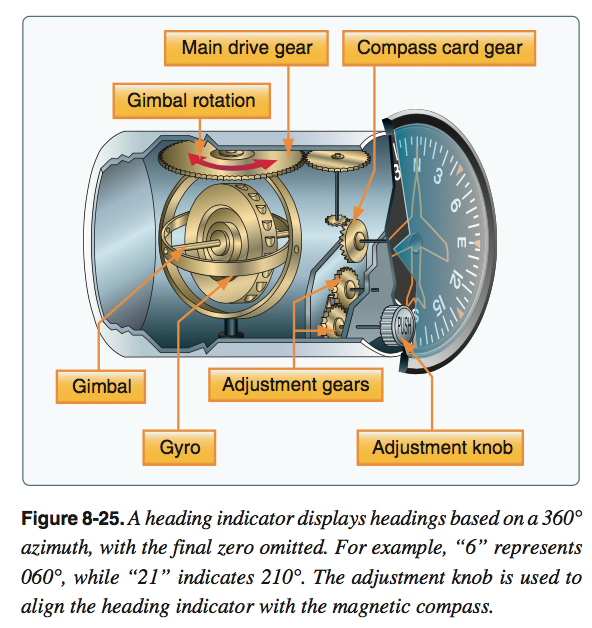
\includegraphics[width=0.5\linewidth]{Figures/Heading Indicator.png}
				\end{figure}
		\subsubsection{Magnetic Compass}
			An aircraft magnetic compass has two small magnets attached to a metal float sealed inside a bowl of clear compass fluid similar to kerosene. A graduated scale, called a card, is wrapped around the float and viewed through a glass window with a lubber line across it. The float and card assembly has a hardened steel pivot in its center that rides inside a special, spring-loaded, hard glass jewel cup. This jewel-and-pivot type mounting allows the float freedom to rotate and tilt up to approximately $18^\circ$ angle of bank. At steeper bank angles, the compass indications are erratic and unpredictable.\footnote{\href[page=227]{./phak.pdf}{PHAK: Flight Instuments - Magnetic Compass}}\\
			Magnetic Compass Errors:
				\begin{enumerate}
					\item Variation: this error comes from the fact that the magnetic poles and geographic poles are not co-located. Magnetic variation is the difference between a heading pointed to magnetic north and true north. An east variation should be subtracted, a west variation should be added.
					\item Deviation: this error is due to the magnetic field induced by an aircraft's electrical system. A compass correction card shows the deviation correction for various headings.
					\item Dip Errors: this error is caused due to the fact that the earth's magnetic field lines are only parallel to the surface at the Earth's magnetic equator. Therefore at any position away from the magnetic equator, a magnetic compass would deflect downward toward the magnetic pole. Therefore, in the Northern hemisphere, compasses are weighted on the Southern (cardinal, Northern magnetic) end to balance this deflection. This weight induces the following two errors.
					\item N/S Turning Errors: the magnetic compass is unevenly weighted, and floats freely so it does not rotate with the plane. As the aircraft turns, the force that results from the magnetic dip causes the float assembly to swing in the same direction that the float turns. The result is a false northerly turn indication. One rule of thumb to correct for this leading error is to stop the turn 15 degrees plus half of the latitude. When turning in a southerly direction, the forces are such that the compass float assembly lags rather than leads. The result is a false southerly turn indication. To correct this lagging error, the aircraft should be allowed to pass the desired heading prior to stopping the turn. The same rule of thumb can be used.
					\item Acceleration Errors: the weighted end of the magnetic compass is resistant to acceleration due to inertia. Therefore when a aircraft is accelerated on an east/west heading, the weighted side, in the reference plane of the aircraft, accelerates rearward. When facing east, the weighted end is to the right of the compass, and when accelerated rearward causes a swing to indicate a turn to the east. When the aircraft decelerated, the weight swings forward, and causes the compass to swing to indicate a turn to the west. The converse is true when facing west.
					\item Oscillation Error: Oscillation is a combination of all of the errors previously mentioned and results in fluctuation of the compass card in relation to the actual heading direction of the aircraft. 
				\end{enumerate}
	\subsection{Systems Instruments}
		\subsubsection{Engine Instruments}
			\begin{itemize}
				\item Tachometer: An instrument that displays engine/propeller speed. In aircraft equipped with a fixed-pitch prop this is also a reading of engine power output.
				\item Manifold Pressure gauge: The gauge measures the absolute pressure of the fuel-air mixture inside the intake manifold and is more correctly a measure of manifold absolute pressure (MAP). At a constant rpm and altitude, the amount of power produced is directly related to the fuel-air mixture being delivered to the combustion chamber. As the throttle setting is increased, more fuel and air flows to the engine and MAP increases.\footnote{\href[page=168]{./phak.pdf}{PHAK: Aircraft Systems - Adjustable-Pitch Propeller}}
				\item Oil Pressure gauge: The oil pressure gauge provides a direct indication of the oil system operation. It ensures the pressure in pounds per square inch (psi) of the oil supplied to the engine. In an aircraft equipped with a variable-pitch propeller, fine pitch corresponds to high oil pressure, and coarse pitch with lower oil pressure.\footnote{\href[page=178]{./phak.pdf}{PHAK: Aircraft Systems - Oil Systems}}
				\item Oil Temperature gauge: High oil temperature indications may signal a plugged oil line, a low oil quantity, a blocked oil cooler, or a defective temperature gauge. Low oil temperature indications may signal improper oil viscosity during cold weather operations.\footnote{\href[page=178]{./phak.pdf}{PHAK: Aircraft Systems - Oil Systems}}
				\item Temperature gauge: A measurement of coolant temperature in liquid cooled engines. High coolant temperature is indicative of inadequate cooling or low coolant levels. Low coolant temperature is most likely a sign of an erroneous sensor.
				\item Fuel Gauge: a measuring device for the amount of fuel in each tank, which is only required to be accurate when empty
				\item Cylinder Head Temperature (CHT): a more accurate measurement of engine temperature than oil temperature. To avoid excessive cylinder head temperatures, increase airspeed, enrich the fuel-air mixture, and/or reduce power. \footnote{\href[page=180]{./phak.pdf}{PHAK: Aircraft Systems - Engine Cooling Systems}}
				\item Exhaust Gas Temperature (EGT): The EGT gauge measures the temperature of the gases at the exhaust manifold. This temperature varies with the ratio of fuel to air entering the cylinders and can be used as a basis for regulating the fuel-air mixture. The EGT gauge is highly accurate in indicating the correct fuel-air mixture setting.\footnote{\href[page=180]{./phak.pdf}{PHAK: Aircraft Systems - Exhaust Systems}}
			\end{itemize}
		\subsubsection{Electrical System Instruments}
			\begin{itemize}
				\item Voltmeter: a measurement of battery voltage. This is kept constant, by means of a voltage regulator, which meters the rate of charge and discharge of the battery.
				\item Ammeter: a measurement of electrical current; when the electrical system is operating correctly this should read positive/zero as the battery is charging.  The ammeter shows if the alternator/ generator is producing an adequate supply of electrical power. It also indicates whether or not the battery is receiving an electrical charge.\footnote{\href[page=192]{./phak.pdf}{PHAK: Aircraft Systems - Electrical System}}
			\end{itemize}
	\subsection{Communications Systems}
		\subsubsection{Radios}
			Operating in and out of a towered airport, as well as in a good portion of the airspace system, requires that an aircraft have two- way radio communication capability. In general aviation, the most common types of radios are VHF. A VHF radio operates on frequencies between 118.0 megahertz (MHz) and 136.975 MHz and is classified as 720 or 760 depending on the number of channels it can accommodate. The 720 and 760 use .025 MHz (25 kilohertz (KHz) spacing (118.025, 118.050) with the 720 having a frequency range up to 135.975 MHz and the 760 reaching up to 136.975 MHz. VHF radios are limited to line of sight transmissions; therefore, aircraft at higher altitudes are able to transmit and receive at greater distances.\footnote{\href[page=358]{./phak.pdf}{PHAK: Airport Operations - Radio Communications}}
		\subsubsection{Transponders} 
			The transponder is the airborne portion of the secondary surveillance radar system. A transponder is also required to operate in certain controlled airspace. A transponder code consists of four numbers from 0 to 7 (4,096 possible codes). There are some standard codes or ATC may issue a four-digit code to an aircraft. When a controller requests a code or function on the transponder, the word ``squawk'' may be used. The ``IDENT'' feature is used by ATC to locate a particular aircraft.\footnote{\href[page=361]{./phak.pdf}{PHAK: Airport Operations - Transponder}}\\
			The following codes are reserved:\footnote{\href[page=168]{./aim.pdf}{AIM 4-1-120 Transponder Operation}}
				\begin{itemize}
					\item 1200 - VFR ``Squawk VFR''
					\item 7500 - Emergency, hijack
					\item 7600 - Emergency, communications failure
					\item 7700 - Emergency, mayday (generic emergency)
					\item 7777 - Military interceptor
				\end{itemize}
			Codes 7500,7600,7700, and 7777 should be avoided from inadvertent selection.\\
			Some transponders are equipped with a Mode C automatic altitude reporting capability, which is required for operation in certain airspace. 
		\subsubsection{ELT}
			An ELT is an Emergency Locator Transmitter. ELTs of various types were developed as a means of locating downed aircraft. These electronic, battery operated transmitters operate on one of three frequencies. These operating frequencies are 121.5 MHz, 243.0 MHz, and the newer 406 MHz. ELTs operating on 121.5 MHz and 243.0 MHz are analog devices. The newer 406 MHz ELT is a digital transmitter that can be encoded with the owner’s contact information or aircraft data. The latest 406 MHz ELT models can also be encoded with the aircraft’s position data which can help SAR forces locate the aircraft much more quickly after a crash. The 406 MHz ELTs also transmits a stronger signal when activated than the older 121.5 MHz ELTs. Analog 121.5/243 MHz ELTs should only be tested during the first 5 minutes after any hour. Pilots are encouraged to monitor 121.5 MHz and/or 243.0 MHz while inflight to assist in identifying possible emergency ELT transmissions. On receiving a signal, report to the nearest air traffic facility.\footnote{\href[page=412]{./aim.pdf}{AIM: 6-2-4 Emergency Locator Transmitter (ELT)}}
		\subsubsection{TCAS, TIS-B, ADS-B, \& FIS-B}
			\paragraph{TCAS: Traffic Alert and Collision Avoidance System} TCAS I provides proximity warning only, to assist the pilot in the visual acquisition of intruder aircraft. No recommended avoidance maneuvers are provided nor authorized as a direct result of a TCAS I warning. TCAS II provides traffic advisories (TAs) and resolution advisories (RAs). Resolution advisories provide recommended maneuvers in a vertical direction (climb or descend only) to avoid conflicting traffic. Each pilot who deviates from an ATC clearance in response to a TCAS II RA must notify ATC of that deviation as soon as practicable and expeditiously return to the current ATC clearance when the traffic conflict is resolved. TCAS does not alter or diminish the pilot’s basic authority and responsibility to ensure safe flight. Since TCAS does not respond to aircraft which are not transponder equipped or aircraft with a transponder failure, TCAS alone does not ensure safe separation in every case.\footnote{\href[page=223]{./aim.pdf}{AIM: 4-4-16 Traffic Alert and Collision Avoidance System (TCAS I \& II)}}
			\paragraph{TIS-B: Traffic Information Service-Broadcast} TIS provides proximity warning only, to assist the pilot in the visual acquisition of intruder aircraft. No recommended avoidance maneuvers are provided nor authorized as a direct result of a TIS intruder display or TIS alert. It is intended for use by aircraft in which TCAS is not required. Since TIS does not respond to aircraft which are not transponder equipped, aircraft with a transponder failure, or aircraft out of radar coverage, TIS alone does not ensure safe separation in every case.\footnote{\href[page=224]{./aim.pdf}{AIM: 4-4-17 Traffic Information Service (TIS)}}\\
			TIS−B is the broadcast of ATC derived traffic information to ADS−B equipped (1090ES or UAT) aircraft from ground radio stations. The source of this traffic information is derived from ground−based air traffic surveillance sensors. TIS−B service will be available throughout the NAS where there are both adequate surveillance coverage from ground sensors and adequate broadcast coverage from ADS−B ground radio stations.\footnote{\href[page=242]{./aim.pdf}{AIM: 4-5-8 Traffic Information Service− Broadcast (TIS−B)}}
			\paragraph{ADS-B: Automatic Dependent Surveillance−Broadcast}Automatic Dependent Surveillance Broadcast (ADS−B) is a surveillance technology deployed throughout the national airspace system. The ADS−B system is composed of aircraft avionics and a ground infrastructure. Onboard avionics determine the position of the aircraft by using the GNSS and transmit its position along with additional informa- tion about the aircraft to ground stations for use by ATC and other ADS−B services. In the United States, ADS−B equipped aircraft exchange information is on one of two frequencies: 978 or 1090 MHz. The 1090 MHz frequency is associated with Mode A, C, and S transponder operations. 1090 MHz transponders with integrated ADS−B functionality extend the transponder message sets with additional ADS−B information.  ADS−B equipment operating on 978 MHz is known as the Universal Access Transceiver (UAT). ADS−B enables improved surveillance ser- vices, both air−to−air and air−to−ground, especially in areas where radar is ineffective due to terrain. \footnote{\href[page=224]{./aim.pdf}{AIM: 4-5-7 Automatic Dependent Surveillance−Broadcast (ADS−B) Services}}
			\paragraph{FIS-B: Flight Information Service - Broadcast (FIS−B)} FIS−B is a ground broadcast service provided through the ADS−B Services network over the 978 MHz UAT data link. The FAA FIS-B system provides pilots and flight crews of properly equipped aircraft with a cockpit display of certain aviation weather and aeronautical information. FIS-B does not replace a preflight weather briefing from a source listed in Paragraph 7−1−2, FAA Weather Services, or inflight updates from an FSS or ATC. FIS-B information may be used by the pilot for the safe conduct of flight and aircraft movement; however, the information should not be the only source of weather or aeronautical information. A pilot should be particularly alert and understand the limitations and quality assurance issues associated with individual products. This includes graphical representation of weather radar imagery, NOTAMs, and TFRs. \footnote{\href[page=243]{./aim.pdf}{AIM: 4-5-9 Flight Information Service− Broadcast (FIS−B)}}
	\subsection{Navigation Systems}
		\subsubsection{Course Deviation Indicator (CDI)}
			\begin{figure}[H]
				\centering
				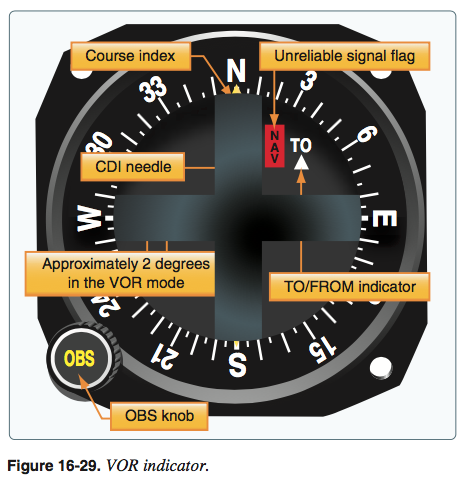
\includegraphics[width=0.5\linewidth]{Figures/CDI.png}
			\end{figure}
			The CDI is found in most training aircraft. It consists of an omnibearing selector (OBS) sometimes referred to as the course selector, a CDI needle (left-right needle), and a TO/ FROM indicator. The course selector is an azimuth dial that can be rotated to select a desired radial or to determine the radial over which the aircraft is flying. In addition, the magnetic course ``TO'' or ``FROM'' the station can be determined. When the course selector is rotated, it moves the CDI or needle to indicate the position of the radial relative to the aircraft. If the course selector is rotated until the deviation needle is centered, the radial (magnetic course ``FROM'' the station) or its reciprocal (magnetic course ``TO'' the station) can be determined. The course deviation needle also moves to the right or left if the aircraft is flown or drifting away from the radial which is set in the course selector. By centering the needle, the course selector indicates either the course ``FROM'' the station or the course ``TO'' the station. If the flag displays a ``TO,'' the course shown on the course selector must be flown to the station. If ``FROM'' is displayed and the course shown is followed, the aircraft is flown away from the station.\footnote{\href[page=411]{./phak.pdf}{PHAK: Navigation - Course Deviation Indicator (CDI)}}
		\subsubsection{Horizontal Situation Indicator (HSI)}
			\begin{wrapfigure}{H}{0.5\linewidth}
				\centering
				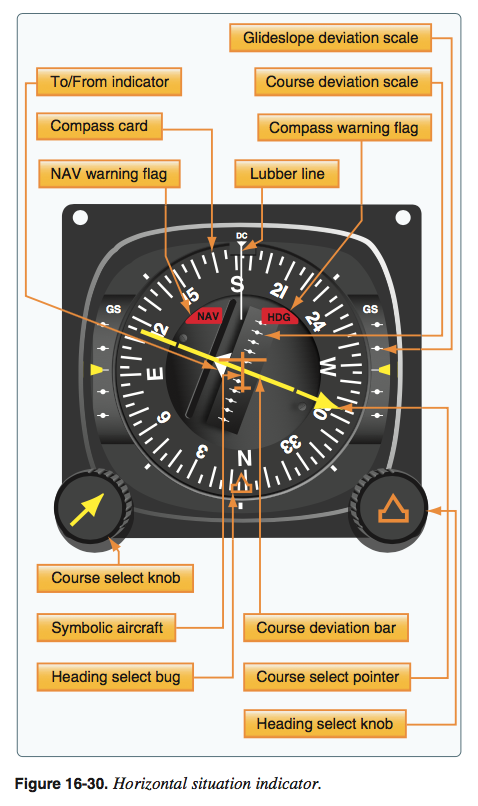
\includegraphics{Figures/HSI.png}
			\end{wrapfigure}
			The HSI is a direction indicator that uses the output from a flux valve to drive the compass card. The HSI combines the magnetic compass with navigation signals and a glideslope. The HSI gives the pilot an indication of the location of the aircraft in relation to the chosen course or radial. The desired course is selected by rotating the course select pointer, in relation to the compass card, by means of the course select knob. The HSI has a fixed aircraft symbol and the course deviation bar displays the aircraft’s position relative to the selected course. The TO/FROM indicator is a triangular pointer. When the indicator points to the head of the course select pointer, the arrow shows the course selected. If properly intercepted and flown, the course takes the aircraft to the chosen facility. When the indicator points to the tail of the course, the arrow shows that the course selected, if properly intercepted and flown, takes the aircraft directly away from the chosen facility.\footnote{\href[page=412]{./phak.pdf}{PHAK: Navigation - Horizontal Situation Indicator}}
		\subsubsection{Radio Magnetic Indicator (RMI)}
			The RMI is a navigational aid providing aircraft magnetic or directional gyro heading and very high frequency omnidirectional range (VOR), GPS, and automatic direction finder (ADF) bearing information.  The pointer indicates the course to the selected NA V AID or waypoint. In Figure 16-31, the green pointer is indicating the station tuned on the ADF. The yellow pointer is indicating the course to a VOR or GPS waypoint. Note that there is no requirement for a pilot to select a course with the RMI. Only the selected navigation source is pointed to by the needle(s).\footnote{\href[page=412]{./phak.pdf}{PHAK: Navigation - Radio Magnetic Indicator (RMI)}}
		\subsubsection{Distance Measuring Equipment (DME)}
			Distance measuring equipment (DME) consists of an ultra high frequency (UHF) navigational aid with VOR/DMEs and VORTACs. It measures, in NM, the slant range distance of an aircraft from a VOR/DME or VORTAC (both hereafter referred to as a VORTAC). Although DME equipment is very popular, not all aircraft are DME equipped. A VOR radial alone merely gives line of position information. With DME, a pilot may precisely locate the aircraft on a given line (radial).\footnote{\href[page=415]{./phak.pdf}{PHAK: Navigation - Distance Measuring Equipment (DME)}}
		\subsubsection{Automatic Direction Finder (ADF)}
			\begin{figure}[H]
			   	\centering
			   	\subfloat{{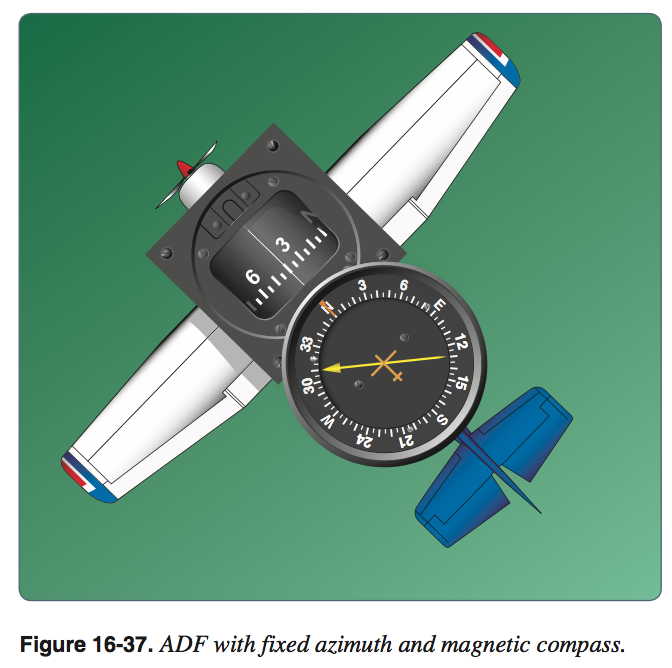
\includegraphics[width=0.5\linewidth]{Figures/ADF 1.png}}}
				\subfloat{{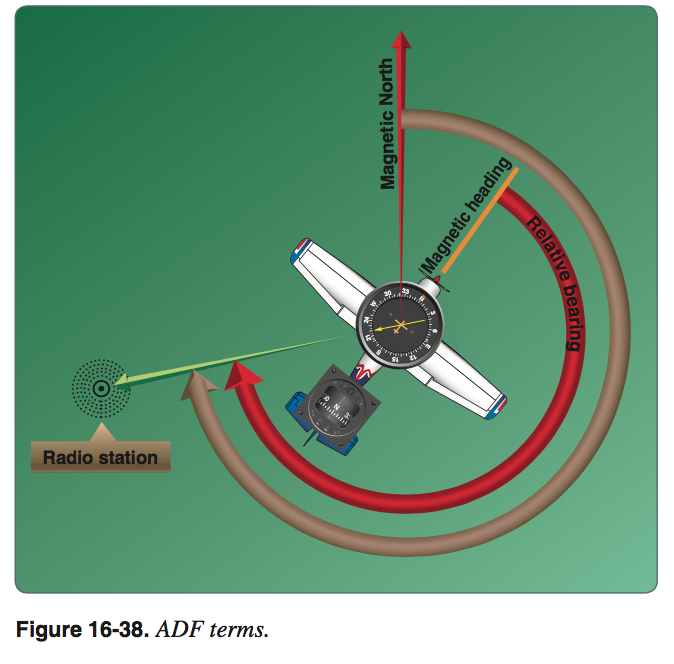
\includegraphics[width=0.5\linewidth]{Figures/ADF 2.png}}}
			\end{figure}
			Many general aviation-type aircraft are equipped with ADF radio receiving equipment. To navigate using the ADF, the pilot tunes the receiving equipment to a ground station known as a nondirectional radio beacon (NDB). The NDB stations normally operate in a low or medium frequency band of 200 to 415 kHz. Standard broadcast stations can also be used in conjunction with ADF. Positive identification of all radio stations is extremely important and this is particularly true when using standard broadcast stations for navigation. NDBs have one advantage over the VOR in that low or medium frequencies are not affected by line-of-sight. The signals follow the curvature of the Earth; therefore, if the aircraft is within the range of the station, the signals can be received regardless of altitude.\footnote{\href[page=417]{./phak.pdf}{PHAK: Navigation - Automatic Direction Finder (ADF)}}

		\subsubsection{GPS}
			GPS is a satellite-based navigation system composed of a network of satellites placed into orbit by the United States Department of Defense (DOD). A GPS receiver must be locked onto the signal of at least three satellites to calculate a two-dimensional position (latitude and longitude) and track movement. With four or more satellites in view, the receiver can determine the user’s three-dimensional position (latitude, longitude, and altitude). Other satellites must also be in view to offset signal loss and signal ambiguity. \footnote{\href[page=86]{./phak.pdf}{PHAK: Aircraft Construction - Global Positioning System (GPS)}}
				\subsubsection{RAIM}
					The GPS receiver verifies the integrity (usability) of the signals received from the GPS constellation through receiver autonomous integrity monitoring (RAIM) to determine if a satellite is providing corrupted information. At least one satellite, in addition to those required for navigation, must be in view for the receiver to perform the RAIM function; thus, RAIM needs a minimum of five satellites in view or four satellites and a barometric altimeter (baro-aiding) to detect an integrity anomaly. For receivers capable of doing so, RAIM needs six satellites in view (or five satellites with baro-aiding) to isolate the corrupt satellite signal and remove it from the navigation solution. \footnote{\href[page=419]{./phak.pdf}{PHAK: Navigation - GPS}}
				\subsubsection{WAAS \& SBAS}
					\begin{itemize}
						\item Wide Area Augmentation System (WAAS): WAAS will allow GPS to be used, as the aviation navigation system, from takeoff through approach when it is complete. Precisely surveyed wide−area reference stations (WRS) are linked to form the U.S. WAAS network. Signals from the GPS satellites are monitored by these WRSs to determine satellite clock and ephemeris corrections and to model the propagation effects of the ionosphere. Each station in the network relays the data to a wide−area master station (WMS) where the correction information is computed. A correction message is prepared and uplinked to a geostationary earth orbit satellite. In addition to providing the correction signal, the WAAS GEO provides an additional pseudorange measurement to the aircraft receiver, improving the availability of GPS by providing, in effect, an additional GPS satellite in view. The integrity of GPS is improved through real−time monitoring, and the accuracy is improved by providing differential corrections to reduce errors. The performance improvement is sufficient to enable approach procedures with GPS/WAAS glide paths (vertical guidance).\footnote{\href[page=61]{./aim.pdf}{AIM: 1-1-18 Wide Area Augmentation System (WAAS)}}
						\item Satellite Based Augmentation System (SBAS): Operationally similar to WAAS, excepting that unlike with WAAS, the correction signal is from satellites only instead of both from ground stations and from satellites.
					\end{itemize}
%done
\newpage
\section{Pre-Flight}
	\subsection{Private Pilot Privileges and Limitations}
		\subsubsection{Eligibility Requirements}
			To be eligible for a private pilot certificate, a person must:
			\footnote{\href{https://www.law.cornell.edu/cfr/text/14/61.103}{14 CFR 61.103 - Eligibility requirements: General}}
				\begin{enumerate}[label=\alph*]
					\item Be at least 17 years of age for a rating in other than a glider or balloon.
					\item Be able to read, speak, write, and understand the English language. 
					\item Receive a logbook endorsement from an authorized instructor who.
						\begin{enumerate}[label=\arabic*]
							\item Conducted the training or reviewed the person's home study on the aeronautical knowledge areas listed in 61.105(b) of this part that apply to the aircraft rating sought; and
							\item Certified that the person is prepared for the required knowledge test.
						\end{enumerate}
					\item Pass the required knowledge test on the aeronautical knowledge areas listed in § 61.105(b) of this part.
					\item Receive flight training and a logbook endorsement from an authorized instructor who:
						\begin{enumerate}[label=\arabic*]
							\item Conducted the training in the areas of operation listed in 61.107(b) of this part that apply to the aircraft rating sought; and
							\item Certified that the person is prepared for the required practical test.
						\end{enumerate}
					\item Meet the aeronautical experience requirements of this part that apply to the aircraft rating sought before applying for the practical test.
					\item Pass a practical test on the areas of operation listed in § 61.107(b) of this part that apply to the aircraft rating sought.
				\end{enumerate}
		\subsubsection{Privileges \& Limitations}
			A private pilot has several privileges and limitations.\footnote{\href{https://www.law.cornell.edu/cfr/text/14/61.113}{14 CFR 61.113 - Private pilot privileges and limitations: Pilot in command.}}
			\begin{enumerate}[label=\alph*]
				\item Except as provided in paragraphs (b) through (h) of this section, no person who holds a private pilot certificate may act as pilot in command of an aircraft that is carrying passengers or property for compensation or hire; nor may that person, for compensation or hire, act as pilot in command of an aircraft.
				\item A private pilot may, for compensation or hire, act as pilot in command of an aircraft in connection with any business or employment if:
					\begin{enumerate}[label=\arabic*]
						\item The flight is only incidental to that business or employment; and
						\item The aircraft does not carry passengers or property for compensation or hire.
					\end{enumerate}
				\item A private pilot may not pay less than the pro rata share of the operating expenses of a flight with passengers, provided the expenses involve only fuel, oil, airport expenditures, or rental fees.
				\item A private pilot may act as pilot in command of a charitable, nonprofit, or community event flight described in \href{https://www.law.cornell.edu/cfr/text/14/91.146}{91.146}.
				\item A private pilot may be reimbursed for aircraft operating expenses that are directly related to search and location operations, provided the expenses involve only fuel, oil, airport expenditures, or rental fees, and the operation is sanctioned and under the direction and control of:
					\begin{enumerate}[label=\arabic*]
						\item A local, State, or Federal agency; or
						\item An organization that conducts search and location operations.
					\end{enumerate}
				\item A private pilot who is an aircraft salesman and who has at least 200 hours of logged flight time may demonstrate an aircraft in flight to a prospective buyer.
				\item A private pilot who meets the requirements of \href{https://www.law.cornell.edu/cfr/text/14/61.69}{61.69} may act as a pilot in command of an aircraft towing a glider or un-powered ultralight vehicle.
			\end{enumerate}
		\subsubsection{Documents}
			To act as a required flight crewmember of a U.S civil aircraft, a pilot must have:\footnote{\href{https://www.law.cornell.edu/cfr/text/14/61.3}{14 CFR 61.3 - Requirement for certificates, ratings, and authorizations}}
				\begin{enumerate}
					\item A pilot certificate, special purpose pilot authorization or temporary certificate
					\item A photo identification that is in that person's physical possession or readily accessible in the aircraft when exercising the privileges of that pilot certificate or authorization. The photo identification must be a:
						\begin{enumerate}
							\item Driver's license issued by a State, the District of Columbia, or territory or possession of the United States;
							\item Government identification card issued by the Federal government, a State, the District of Columbia, or a territory or possession of the United States;
							\item Official passport;
						\end{enumerate}
					\item A medical certificate, with certain exceptions. A medical certificate is not required for student pilots or if operating under the provisions of basic med.
				\end{enumerate}
			\paragraph{Medical Certificate}
				A medical certificate comes in three classes, with different durations of validity and sets of privileges.\footnote{\href{https://www.law.cornell.edu/cfr/text/14/61.23}{14 CFR 61.23 - Medical certificates: Requirement and duration.}}
				\begin{enumerate}
					\item A first class is required to exercise ATPL privileges as PIC. A first class is valid for 12 months if issued under the age of 40, and 6 months over the age of forty. A first class is simultaneously a second and third class medical certificate.
					\item A second class is required to exercise ATPL privileges as SIC or a commercial pilot certificate. A second class is valid for 12 months. A second class is simultaneously a third class medical certificate.
					\item A third class is required to exercise a recreational pilot certificate, a private pilot certificate, a flight instructor certificate (when acting as pilot in command or a required pilot flight crewmember in operations other than glider or balloon). It is valid for 5 years if issued under the age of 40, and 2 years otherwise.
				\end{enumerate}
		\subsubsection{Additional Endorsements \& Type Ratings}
			These additional endorsements are logbook endorsements that require additional ground training and/or flight training. These are required to act as PIC in the following set of aircraft:\footnote{\href{https://www.law.cornell.edu/cfr/text/14/61.31}{14 CFR 61.31 - Type rating requirements, additional training, and authorization requirements.}}
			\begin{enumerate}
				\item High Performance: A high-performance airplane has one or more engines with at least 200 HP.
				\item Tailwheel
				\item High-Altitude: Required to operate a pressurized aircraft that has a service ceiling or maximum operating altitude above 25000 MSL.
				\item Complex: A complex airplane has retractable landing gear, flaps, and a controllable pitch propeller; including airplanes equipped with a Full-authority digital engine control.
			\end{enumerate}

			A type rating is required to act as PIC or SIC in any large aircraft (> 12500 lbs), turbojet powered airplane, or other aircraft specified by the FAA.

			W.r.t certification, airplanes are broken up into the following designations:\footnote{\href{https://www.law.cornell.edu/cfr/text/14/1.1}{14 CFR 1.1 - General Definitions}}

			\begin{itemize}
				\item Category: broad classification of aircraft (airplane, rotorcraft, glider, lighter than air, etc.)
				\item Class: a classification of aircraft with similar operating characteristics (ASEL, AMEL, LTA-Balloon, etc.)
				\item Type: A specific make and model of aircraft including modifications that do not change its handling or characteristics.
			\end{itemize}

		\subsubsection{Currency}
			For a pilot to act as a PIC for an aircraft they must:
				\begin{enumerate}
					\item Within the past 24 months, completed a flight review\footnote{\href{https://www.law.cornell.edu/cfr/text/14/61.56}{14 CFR 61.56 - Flight review}}
						\begin{enumerate}
							\item A flight review consists of a minimum of 1 hour of flight training and 1 hour of ground training. 
							\item A flight review is not required if one of the following are accomplished: 
								\begin{enumerate}
									\item A pilot proficiency check or practical test conducted by an examiner, an approved pilot check airman, or a U.S. Armed Force, for a pilot certificate, rating, or operating privilege.
									\item A practical test conducted by an examiner for the issuance of a flight instructor certificate, an additional rating on a flight instructor certificate, renewal of a flight instructor certificate, or reinstatement of a flight instructor certificate.
								\end{enumerate}
						\end{enumerate}
					\item To carry passengers during the day:\footnote{\href{https://www.law.cornell.edu/cfr/text/14/61.57}{14 CFR 61.57(a)- Recent flight experience: Pilot in command, General experience.}}
						\begin{enumerate}
							\item Made at least three takeoffs and three landings within the preceding 90 days.
							\item The person acted as the sole manipulator of the flight controls.
							\item  The required takeoffs and landings were performed in an aircraft of the same category, class, and type (if a type rating is required), and, if the aircraft to be flown is an airplane with a tailwheel, the takeoffs and landings must have been made to a full stop in an airplane with a tailwheel.
						\end{enumerate}
					\item To carry passengers at night:\footnote{\href{https://www.law.cornell.edu/cfr/text/14/61.57}{14 CFR 61.57(b)- Recent flight experience: Pilot in command, Night takeoff and landing experience.}}
						\begin{enumerate}
							\item within the preceding 90 days that person has made at least three takeoffs and three landings to a full stop during the period beginning 1 hour after sunset and ending 1 hour before sunrise.
							\item That person acted as sole manipulator of the flight controls.
							\item The required takeoffs and landings were performed in an aircraft of the same category, class, and type (if a type rating is required).
						\end{enumerate}
				\end{enumerate}
			\subsubsection{Logging \& Acting as PIC}
	\subsection{Required Documents and Equipment (Airworthiness)}
		The term “airworthy” means that the aircraft and its component parts meet the airplane’s type design or is in a properly altered configuration and is in a condition for safe operation. The inspection has two parts and involves the pilot inspecting the airplane’s airworthiness status and a visual preflight inspection of the airplane following the AFM/POH to determine the required items for inspection.\footnote{\href[page=32]{./afh.pdf}{AFH: Ground Operations - Preflight Assessment of the Aircraft}} \\
		The owner/operator is primarily responsible for maintenance, but the pilot is (solely) responsible for determining the airworthiness (and/or safety) of the airplane for flight.\footnote{\href{https://www.law.cornell.edu/cfr/text/14/91.403}{91.403 General.}}\footnote{\href{https://www.law.cornell.edu/cfr/text/14/91.405}{91.405 Maintenance required.}}\\
		A special flight permit, issued from a FSDO is required when operating an aircraft that does not meet airworthiness requirements.\footnote{\href{https://www.law.cornell.edu/cfr/text/14/21.197}{14 CFR 21.197 - Special flight permits.}}\\
		If a piece of equipment is found to be inoperative, and is not required for an aircraft's airworthiness, the equipment must be deactivated and placarded as ``inoperative''.\footnote{\href{https://www.law.cornell.edu/cfr/text/14/91.213}{14 CFR 91.213 - Inoperative instruments and equipment.}}
		\subsubsection{Required Documents}
			\begin{itemize}
				\item \textbf{A}irworthiness Certificate displayed at the cabin or cockpit entrance so that it is legible to passengers or crew. \footnote{\href{https://www.law.cornell.edu/cfr/text/14/91.203}{91.203 Civil aircraft: Certifications required. (a.1,b)}}
				\item \textbf{R}egistration Certificate \footnote{\href{https://www.law.cornell.edu/cfr/text/14/91.203}{91.203 Civil aircraft: Certifications required. (a.2)}}
				\item \textbf{R}adiotelephone Operator Permit
				\item \textbf{O}perating Limitations: AFM/POH, placards and markings.\footnote{\href{https://www.law.cornell.edu/cfr/text/14/91.9}{14 CFR 91.9 - Civil aircraft flight manual, marking, and placard requirements.}} This includes a compass deviation card\footnote{\href{https://www.law.cornell.edu/cfr/text/14/23.1547}{14 CFR 23.1547 - Magnetic direction indicator.}} and an external data plate/serial number.\footnote{\href{https://www.law.cornell.edu/cfr/text/14/45.11}{14 CFR 45.11 - Marking of products.}}
				\item \textbf{W}eight and balance, and performance data. \footnote{\href{https://www.law.cornell.edu/cfr/text/14/23.1589}{14 CFR 23.1589 - Loading information.}}\footnote{\href{https://www.law.cornell.edu/cfr/text/14/91.103}{14 CFR 91.103 - Preflight action}}
			\end{itemize}
		\subsubsection{Required Maintenance}
			An annual inspection is a complete inspection of an aircraft and engine, required by the Code of Federal Regulations, to be accomplished every 12 calendar months on all certificated aircraft. Only an A\&P technician holding an Inspection Authorization can conduct an annual inspection. A 100 hour inspection is identical in scope, but can be performed by any A\&P mechanic.\footnote{\href[page=324]{./afh.pdf}{AFH: Glossary}} The 100-hour limitation may be exceeded by no more than 10 hours when en-route to a place the inspection could be done.\footnote{\href{https://www.law.cornell.edu/cfr/text/14/91.409}{14 CFR 91.409 - Inspections.}} \\
			Preventative maintenance is defined by 14 CFR Part 43.\footnote{\href{https://www.law.cornell.edu/cfr/text/14/appendix-A_to_part_43\#c}{14 CFR Appendix A to Part 43, Major Alterations, Major Repairs, and Preventive Maintenance}} Simple actions such as removal, installation, and repair of landing gear tyres may be performed by Private Pilots or better, so long as the aircraft is not being used in air carrier service.
			\begin{itemize}
				\item \textbf{A}nnual Inspection within the preceding 12 calendar months.\footnote{\href{https://www.law.cornell.edu/cfr/text/14/91.409}{14 CFR 91.409 - Inspections.}}
				\item \textbf{A}irworthiness directives and life-limited parts complied with as required.\footnote{\href{https://www.law.cornell.edu/cfr/text/14/91.403}{14 CFR 91.403 - General.}}\footnote{\href{https://www.law.cornell.edu/cfr/text/14/91.417}{14 CFR 91.417 - Maintenance records.}}
				\item \textbf{V}OR equipment check every 30 days, for IFR operations. At a VOR testing location maximum permissible error $\pm 4^\circ$. Airborne check maximum permissible error $\pm 6^\circ$.\footnote{\href{https://www.law.cornell.edu/cfr/text/14/91.171}{14 CFR 91.171 - VOR equipment check for IFR operations.}}
				\item \textbf{1}00-hour inspection, if used for hire or flight instruction in aircraft provided by CFI.\footnote{\href{https://www.law.cornell.edu/cfr/text/14/91.409}{14 CFR 91.409 - Inspections.}}
				\item \textbf{A}ltimeter, altitude reporting equipment, and static pressure systems tested and inspected, for IFR operations, every 24 calendar months.\footnote{\href{https://www.law.cornell.edu/cfr/text/14/91.411}{14 CFR 91.411 - Altimeter system and altitude reporting equipment tests and inspections.}}
				\item \textbf{T}ransponder tests and inspections every 24 calendar months.\footnote{\href{https://www.law.cornell.edu/cfr/text/14/91.413}{14 CFR 91.413 - ATC transponder tests and inspections.}}
				\item \textbf{E}LT, operation and battery condition inspected every 12 calendar months.\footnote{\href{https://www.law.cornell.edu/cfr/text/14/91.207}{14 CFR 91.207 - Emergency locator transmitters.}}
			\end{itemize}
		\subsubsection{Required Equipment, Day VFR}
			For VFR flight during the day the following is required:\footnote{\href{https://www.law.cornell.edu/cfr/text/14/91.205\#a}{14 CFR 91.205 (a) - Powered civil aircraft with standard category U.S. airworthiness certificates: Instrument and equipment requirements.}}
			\begin{itemize}
				\item \textbf{A}nti-Collision light system, flashing red or white for small airplanes certificated after March 11, 1996.
				\item \textbf{T}achometer for each engine
				\item \textbf{O}il pressure gauge 
				\item \textbf{M}anifold Pressure gauge
				\item \textbf{A}ltimeter
				\item \textbf{T}emperature gauge, for each liquid cooled engine
				\item \textbf{O}il Temperature gauge, for each air cooled engine
				\item \textbf{F}uel gauge indicating the quantity in each tank
				\item \textbf{F}lotation gear, if operated for hire over water beyond power-off gliding distance
				\item \textbf{L}anding gear position indicator, if the airplane has retractable gear
				\item \textbf{A}irspeed indicator
				\item \textbf{M}agnetic direction indicator
				\item \textbf{E}mergency locator transmitter, after June 21 1995. Batteries used in the ELT must be replaced (or recharged, if the batteries are rechargeable) when the transmitter has been in use for more than 1 cumulative hour; or when 50 percent of their useful life (or, for rechargeable batteries, 50 percent of their useful life of charge) has elapsed.\footnote{\href{https://www.law.cornell.edu/cfr/text/14/91.207}{14 CFR 91.207 - Emergency locator transmitters.}}
				\item \textbf{S}afety belts (and shoulder harnesses for each front seat in an aircraft manufactured after July 18, 1978, all seats after December 12 1986)
			\end{itemize}
		\subsubsection{Required Equipment, Night VFR}
			For VFR flight during the night the following is required:\footnote{\href{https://www.law.cornell.edu/cfr/text/14/91.205\#c}{14 CFR 91.205 (c) - Powered civil aircraft with standard category U.S. airworthiness certificates: Instrument and equipment requirements.}}
			\begin{itemize}
				\item \textbf{F}uses, or circuit breakers
				\item \textbf{L}anding lights, if operated for hire
				\item \textbf{A}nti-collision lights, for all night operations
				\item \textbf{P}osition lights
				\item \textbf{S}ource of power (battery or alternator)
			\end{itemize}
	\subsection{Performance Calculations}
		\subsubsection{Weight \& Balance}
			\paragraph{Weight} Any item aboard an aircraft that increases the total weight is undesirable for performance. An overloaded aircraft may not be able to leave the ground, or if it does become airborne, it may exhibit unexpected and unusually poor flight characteristics. 
			\paragraph{Centre of Gravity} CG is simply the average position of all the mass in the aircraft. Mathematically it is: $$\sum_i \frac{1}{M} m_i\cdot r_i $$ CG is typically only calculated along the longitudinal axis. Every aircraft has a \textbf{basic empty weight}, \textbf{lever arm}, and \textbf{moment/torque/action} defined. Any additional weight loaded onto an aircraft has associated values of weight, lever arm and moment, and will consequently change the position of the aircraft's centre of gravity.

			There are two constraints to weight and balance calculations; maximum takeoff weight (and to a lesser extent maximum landing weight, forward CG limits and aft CG limits. An overloaded aircraft has the following performance deficiencies:
				\begin{multicols}{2}
					\begin{enumerate}
						\item Higher takeoff speed
						\item Longer takeoff run
						\item Reduced rate and angle of climb
						\item Lower maximum altitude
						\item Shorter range
						\item Reduced cruising speed
						\item Reduced maneuverability
						\item Higher stalling speed
						\item Higher approach and landing speed
						\item Longer landing roll
						\item Excessive weight on the nose wheel or tail wheel
					\end{enumerate}
				\end{multicols}
			If the CG is displaced too far forward on the longitudinal axis, a nose-heavy condition will result. Conversely, if the CG is displaced too far aft on the longitudinal axis, a tail heavy condition results. It is possible that the pilot could not control the aircraft if the CG location produced an unstable condition. In extreme cases, a CG location that is beyond the forward limit may result in nose heaviness, making it difficult or impossible to flare for landing. In addition to decreased static and dynamic longitudinal stability, other undesirable effects caused by a CG location aft of the allowable range may include extreme control difficulty, violent stall characteristics, and very light control forces which make it easy to overstress an aircraft inadvertently. As the CG moves aft, a less stable condition occurs, which decreases the ability of the aircraft to right itself after maneuvering or turbulence.\footnote{\href[page=248]{./phak.pdf}{PHAK: Weight \& Balance}} Some aircraft have weight dependent fore and aft CG limits.
		\subsubsection{Pressure \& Density Altitude}
			\paragraph{Pressure altitude} is the height above the standard datum 29.8 112 plane (SDP). The aircraft altimeter is essentially a sensitive barometer calibrated to indicate altitude in the standard 29.92 0 atmosphere. If the altimeter is set for 29.92 in Hg, the altitude indicated is the pressure altitude—the altitude in the standard atmosphere corresponding to the sensed pressure. A good rule of thumb is that for every $\pm 0.01$ in Hg, pressure altitude changes from true altitude by $\mp 10$ feet.
			\paragraph{Density Altitude} is pressure altitude corrected for non-standard temperatures. As the density of the air increases (lower density altitude), aircraft performance increases. Conversely, as air density decreases (higher density altitude), aircraft performance decreases. A decrease in air density means a high density altitude; an increase in air density means a lower density altitude.
			In tandem, density and pressure altitude affect aircraft performance; generally higher values of density and pressure altitude decrease an aircraft's performance.
		\subsubsection{Takeoff \& Landing Data}
			The minimum takeoff distance  and landing distance is of primary interest in the operation of any aircraft because it defines the runway requirements. Takeoff distance is a function of density altitude (because lift is a function of air density), take off weight, wind, runway slope, and obstacle height. Landing distance is a function of density altitude, landing weight, wind, runway slope, and obstacle height. A calculation of these values should be performed for every flight, and compared to runway lengths available. These calculations are performed using the data provided in the AFM/POH. 
		\subsubsection{Performance Tables}
			Climb performance data and cruise performance data are also published in an aircraft's POH/AFM. Climb performance is linked to density altitude, as rarefied air produces less lift for a given angle of attack. Generally climb performance diminishes as altitude increases. Particularly in mountainous terrain, an aircraft's climb performance will determine whether certain areas can be safely navigated. If terrain rises faster than the airplane can climb, an impact is inevitable. \\
			Cruise performance data is an important factor in planning cross-country flights. Generally cruise performance information is a function of density altitude, air temperature, and engine power. The relevant output variables are fuel flow rate, and true airspeed. These in turn can be used to calculate the time en route, and to determine what altitude or power setting may be most favorable for the atmospheric conditions on a given route.
	\subsection{Weather Briefings}
		Prior to every flight, pilots should gather all information vital to the nature of the flight. This includes an appropriate weather briefing obtained from a specialist at a FSS. For weather specialists to provide an appropriate weather briefing, they need to know which of the three types of briefings is needed—standard, abbreviated, or outlook. A standard briefing provides the most complete information and a more complete weather picture. This type of briefing should be obtained prior to the departure of any flight and should be used during flight planning. An abbreviated briefing is a shortened version of the standard briefing. It should be requested when a departure has been delayed or when weather information is needed to update the previous briefing. An outlook briefing should be requested when a planned departure is 6 hours or more away. It provides initial forecast information that is limited in scope due to the time frame of the planned flight. This type of briefing is a good source of flight planning information that can influence decisions regarding route of flight, altitude, and ultimately the go/no-go decision.\footnote{\href[page=317]{./phak.pdf}{PHAK: Aviation Weather Services - Weather Briefing}}
		\subsubsection{Weather Data}
			A variety of weather data types are available to pilots:
				\begin{enumerate}
					\item Surface analysis chart: depict surface weather observations including sea level pressure, the positions of highs, lows, ridges, troughs, and fronts.
					\item Weather depiction chart: a plot of weather conditions at METAR stations that depicts the weather category (VFR, Marginal VFR, IFR and Low IFR)
					\item Short-range surface prognostic chart: a forecast of surface pressure systems, fronts, and precipitation for 60 hours in the future, at intervals of 12,18,24,48, and 60 hours.
					\item Significant weather prognostic chart (SIGWX): a forecast of aviation hazards FL240 and below (low-level), and 10000 ft MSL to FL450 (mid-level); including weather flying categories, turbulence, and freezing levels.
					\item Convective outlook chart: depicts areas forecast to have the potential for severe (tornado, wind gusts 50 kts or greater, or hail 3/4 in diameter size or greater), and non-severe convective activity.
					\item Constant pressure analysis chart: A depiction of temperature, dew point, and wind along a surface of constant pressure. 
				\end{enumerate}
		\subsubsection{Aviation Weather Reports \& Forecasts}
			\begin{enumerate}
				\item METAR (Aviation Routine Weather Report): A METAR is an observation of current surface weather reported in a standard international format.\footnote{\href[page=318]{./phak.pdf}{PHAK: Aviation Weather Services - Aviation Routine Weather Report (METAR)}}
					\begin{itemize}
						\item Type of report: either routine at regular time intervals or a SPECI to indicate a rapid change or critical information
						\item Station identifier: the ICAO identifier for the METAR location
						\item Date and time of report in UTC
						\item Modifier: AUTO for automated source, AO1 for no precipitation discriminator, AO2 for a precipitation discriminator. COR indicates a corrected report.
						\item Wind: aaabbbKTGcc; to mean that winds are from aaa$^\circ$ true at a speed of bbb kts, gusting cc kts. If the wind is variable the direction will be listed as VRB.
						\item Visibility: ground visibility, reported in statute miles. This may also include RVR (runway visual range)
						\item Weather: various codes representing different weather conditions, intensity and vicinity.
						\item Sky condition: reported in the sequence of amount, height, and type or indefinite ceiling/height (vertical visibility) (BKN008 OVC012CB, VV003). The heights of the cloud bases are reported with a three-digit number in hundreds of feet AGL.  The types of clouds, specifically towering cumulus (TCU) or cumulonimbus (CB) clouds, are reported with their height.
						\item Temperature and dew point: the air temperature and dew point are always given in degrees Celsius (C) or (18/17). Temperatures below $0^\circ$C are preceded by the letter ``M'' to indicate minus.
						\item Altimeter setting: reported in inches of mercury A2970 for 29.70 in Hg or QNH1013 for 1013 HPa.
						\item Remarks: labeled with RMK including any information not previously stated
					\end{itemize}
				\item TAF (Terminal Aerodrome Forecasts) A TAF is a report established for the five statute mile radius around an airport. TAF reports are usually given for larger airports. Each TAF is valid for a 24 or 30-hour time period and is updated four times a day at 0000Z, 0600Z, 1200Z, and 1800Z. The TAF utilizes the same descriptors and abbreviations as used in the METAR report. The following are unique to a TAF\footnote{\href[page=321]{./phak.pdf}{PHAK: Aviation Weather Services - Terminal Aerodrome Forecasts (TAF)}}:
					\begin{itemize}
						\item Forecast change group: for any significant weather change forecast to occur during the TAF time period, the expected conditions and time period are included in this group. This information may be shown as from (FM), and temporary (TEMPO).
						\item  PROBxx: a given percentage that describes the probability of thunderstorms and precipitation occurring in the coming hours.
					\end{itemize}
				\item MOS (Model Output Statistics): a computer generated forecast based on NWS weather models, upon which TAFs are based.
				\item AIRMET: AIRMETs (WAs) are examples of inflight weather advisories that are issued every 6 hours with intermediate updates issued as needed for a particular area forecast region. Sierra is the AIRMET code used to denote IFR and mountain obscuration; Tango is used to denote turbulence, strong surface winds, and low-level wind shear; and Zulu is used to denote icing and freezing levels. \footnote{\href[page=323]{./phak.pdf}{PHAK: Aviation Weather Services - AIRMET}}
				\item SIGMET: SIGMETs (WSs) are inflight advisories concerning non- convective weather that is potentially hazardous to all aircraft. They report weather forecasts that include severe icing not associated with thunderstorms, severe or extreme turbulence or clear air turbulence (CAT) not associated with thunderstorms, dust storms or sandstorms that lower surface or inflight visibilities to below three miles, and volcanic ash. A SIGMET is issued under an alphabetic identifier, from November through Yankee. The first issuance of a SIGMET is designated as an Urgent Weather SIGMET (UWS). Reissued SIGMETs for the same weather phenomenon are sequentially numbered until the weather phenomenon ends.\footnote{\href[page=324]{./phak.pdf}{PHAK: Aviation Weather Services - SIGMET}}
				\item PIREPs (Pilot Weather Reports): PIREPs provide valuable information regarding the conditions as they actually exist in the air, which cannot be gathered from any other source. Pilots can confirm the height of bases and tops of clouds, locations of wind shear and turbulence, and the location of inflight icing. If the ceiling is below 5,000 feet, or visibility is at or below five miles.\footnote{\href[page=320]{./phak.pdf}{PHAK: Aviation Weather Services - Pilot Weather Reports (PIREPs)}}
					\begin{multicols}{2}
					\begin{enumerate}[label=\arabic*]
						\item 3-letter station identifier
						\item UA for a routine PIREP, UUA-Urgent PIREP
						\item /OV Location 
						\item /TM Time in UTC
						\item /FL altitude or flight level
						\item /TP Type aircraft
						\item /SK Sky cover/cloud layers
						\item /WX weather
						\item /TA Air temperature in celcius
						\item /WV wind
						\item /TB turbulence category and type (none,light,moderate,severe,extreme), clear air turbulence (CAT)
						\item /IC icing category and type (light,moderate,severe), (clear,rime) 
						\item /RM remarks
					\end{enumerate}
					\end{multicols}
			\end{enumerate}
		\subsubsection{NOTAMs \& TFRs}
			\begin{enumerate}
				\item Notices to Airmen (NOTAM): Time-critical aeronautical information, which is of a temporary nature or not sufficiently known in advance to permit publication, on aeronautical charts or in other operational publications receives immediate dissemination by the NOTAM system. It includes such information as taxiway and runway closures, construction, communications, changes in status of navigational aids, and other information essential to planned en route, terminal, or landing operations.\footnote{\href[page=341]{./phak.pdf}{PHAK: Airport Operations - Notices to Airmen (NOTAM)}}
				\item Temporary Flight Restrictions (TFRs): A flight data center (FDC) Notice to Airmen (NOTAM) is issued to designate a TFR. The NOTAM begins with the phrase ``FLIGHT RESTRICTIONS'' followed by the location of the temporary restriction, effective time period, area defined in statute miles, and altitudes affected.\footnote{\href[page=382]{./phak.pdf}{PHAK: Airspace - Temporary Flight Restrictions (TFR)}}
			\end{enumerate}
	\subsection{Required Pre-Flight Actions}
		For a flight under IFR or a flight not in the vicinity of an airport each pilot in command shall, before beginning a flight, become familiar with all available information concerning that flight.\footnote{\href{https://www.law.cornell.edu/cfr/text/14/91.103}{14 CFR 91.103 - Preflight action.}} This information must include:
		\begin{itemize}
			\item \textbf{N}OTAMSs
			\item \textbf{W}eather reports and forecasts
			\item \textbf{K}nown ATC traffic delays
			\item \textbf{R}unway lengths at airports of intended use
			\item \textbf{A}lternates available if the planned flight cannot be completed
			\item \textbf{F}uel requirements
			\item \textbf{T}akeoff and landing distance data
		\end{itemize}
%done
\newpage
\section{Airport Operations}
	\subsection{Airport Information}
		\subsubsection{Airport Types}
			There are two types of airports, towered and non-towered airports.\\

			A \textbf{towered} airport has an operating control tower. Air Traffic control is responsible for managing air traffic flow. Pilots operating from a towered airport are required to establish or maintain two-way radio communication with ATC and to acknowledge and comply with their instructions. Pilots must advise ATC if they cannot comply with the instructions issued and request amended instructions. A pilot may deviate from an air traffic instruction in an emergency, but must advise ATC of the deviation as soon as possible.

			\textbf{Non-towered} airports do not have a control tower. This does not mean however, that they are in uncontrolled airspace. Two-way radio communications are not explicitly required while operating at a non-towered airport. A Common Traffic Advisory Frequency (CTAF), is used for pilots to announce their position and intention for the benefit of other airport users. The CTAF may be a Universal Integrated Community (UNICOM), MULTICOM (122.9), Flight Service Station (FSS), or tower frequency as published. On pilot request, UNICOM stations may provide pilots with weather information, wind direction, the recommended runway, or other necessary information.

			These airports come in several varieties: they may be either civil, millitary or private airports or seaplane base.
		\subsubsection{Airport Data}
			\paragraph{Airport Diagrams}
				Airport diagrams give a pictoral depiction of an airport, and list some, but not all important information about the airport. Not all airports have published airport diagrams. An airport diagram is best used to navigate around an airport. Airport diagrams are only updated when major changes occur.\\
				Some pieces of information that can be found on an aiport diagram:
				\begin{multicols}{2}
				\begin{enumerate}
					\item Airport name, and associatedcity name.
					\item Associated frequencies (ground, tower, ckearance delivery, ATIS)
					\item Elevation of touchdown zones, and field elevation.
					\item Runway dimensions, grades, materials, numbers, and positions of displaced thresholds or movement areas. 
					\item Taxiway designations
					\item Airport hot-spots
					\item Position of control towers, or lighted beacon.
				\end{enumerate}
				\end{multicols}
				\begin{figure}
					\centering
					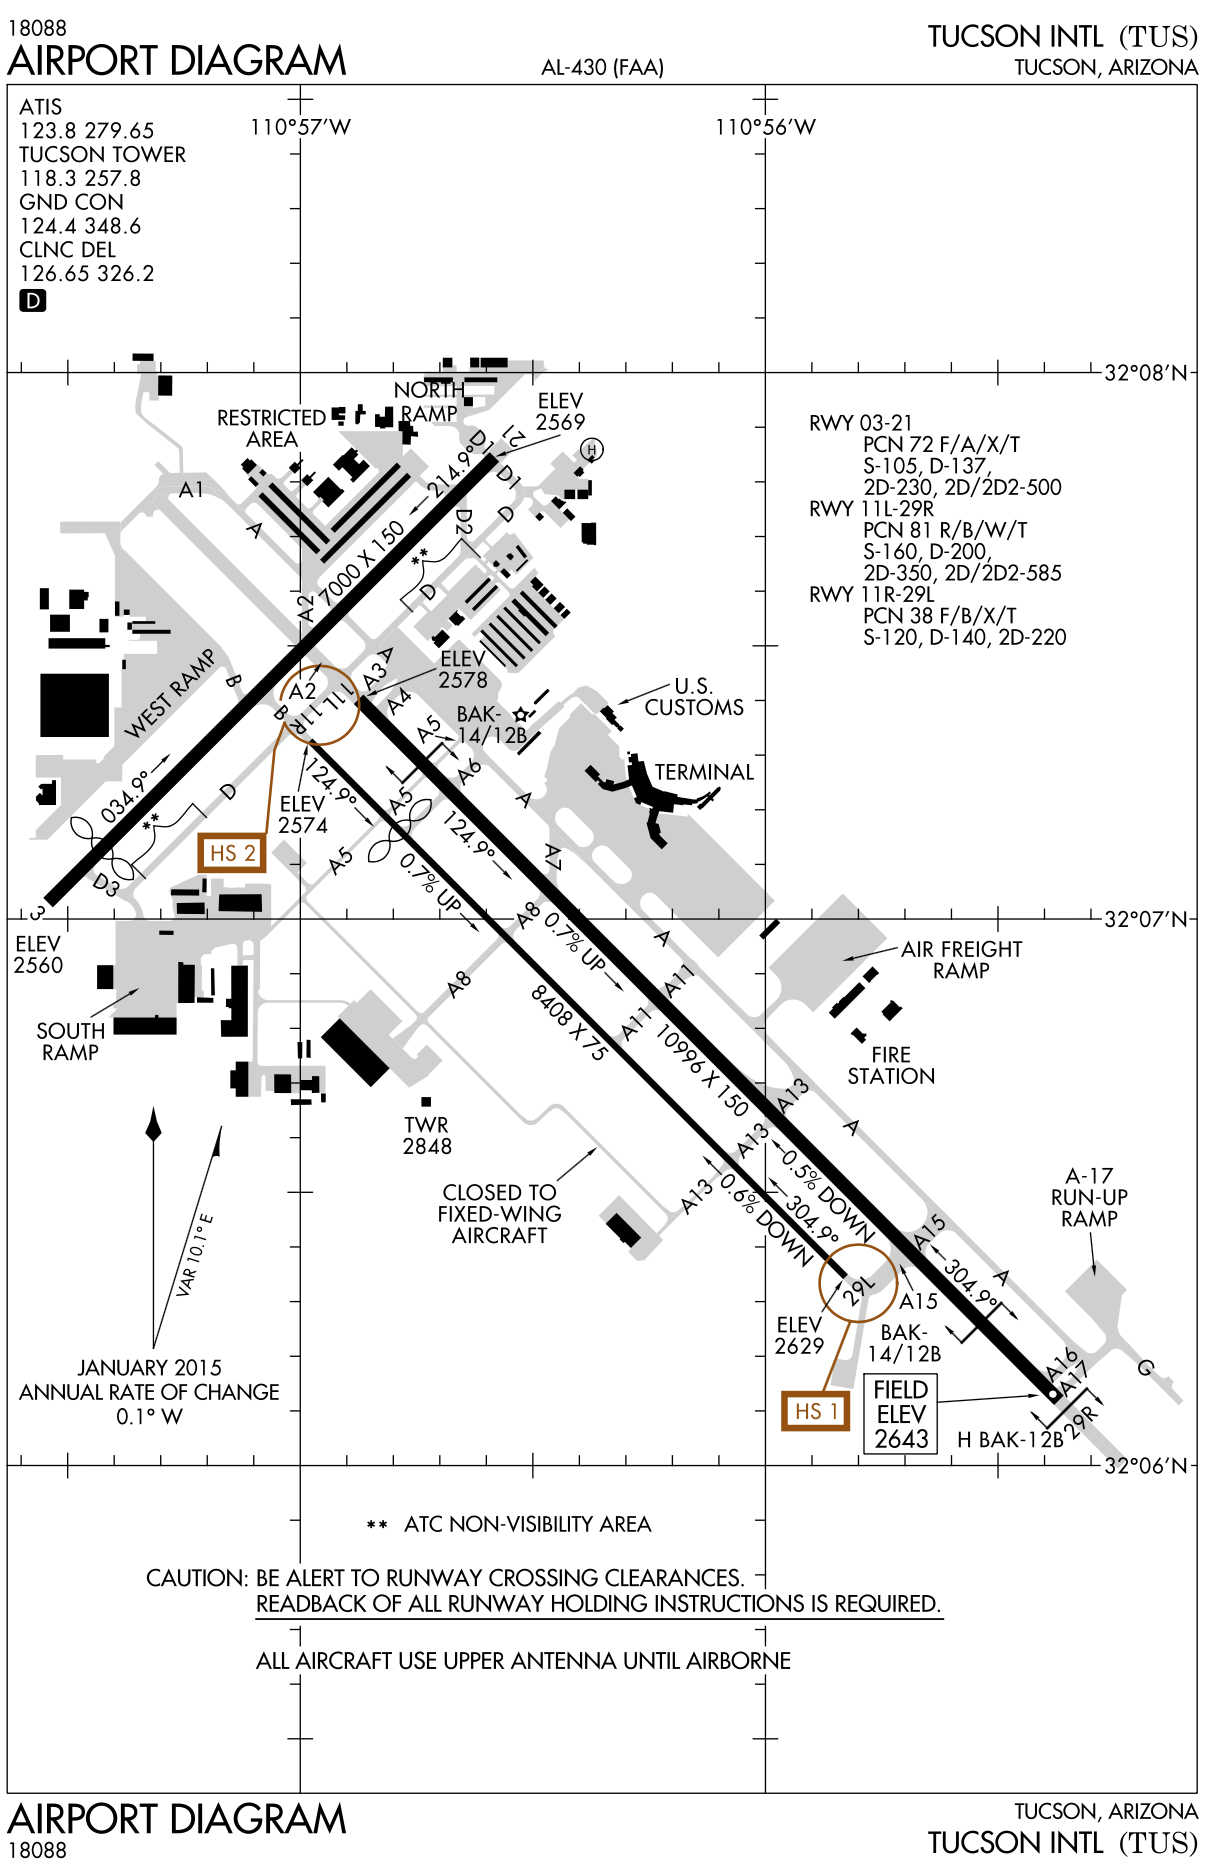
\includegraphics[width=\linewidth]{Airport Diagram.png}
				\end{figure}
				\begin{figure}
					\centering
					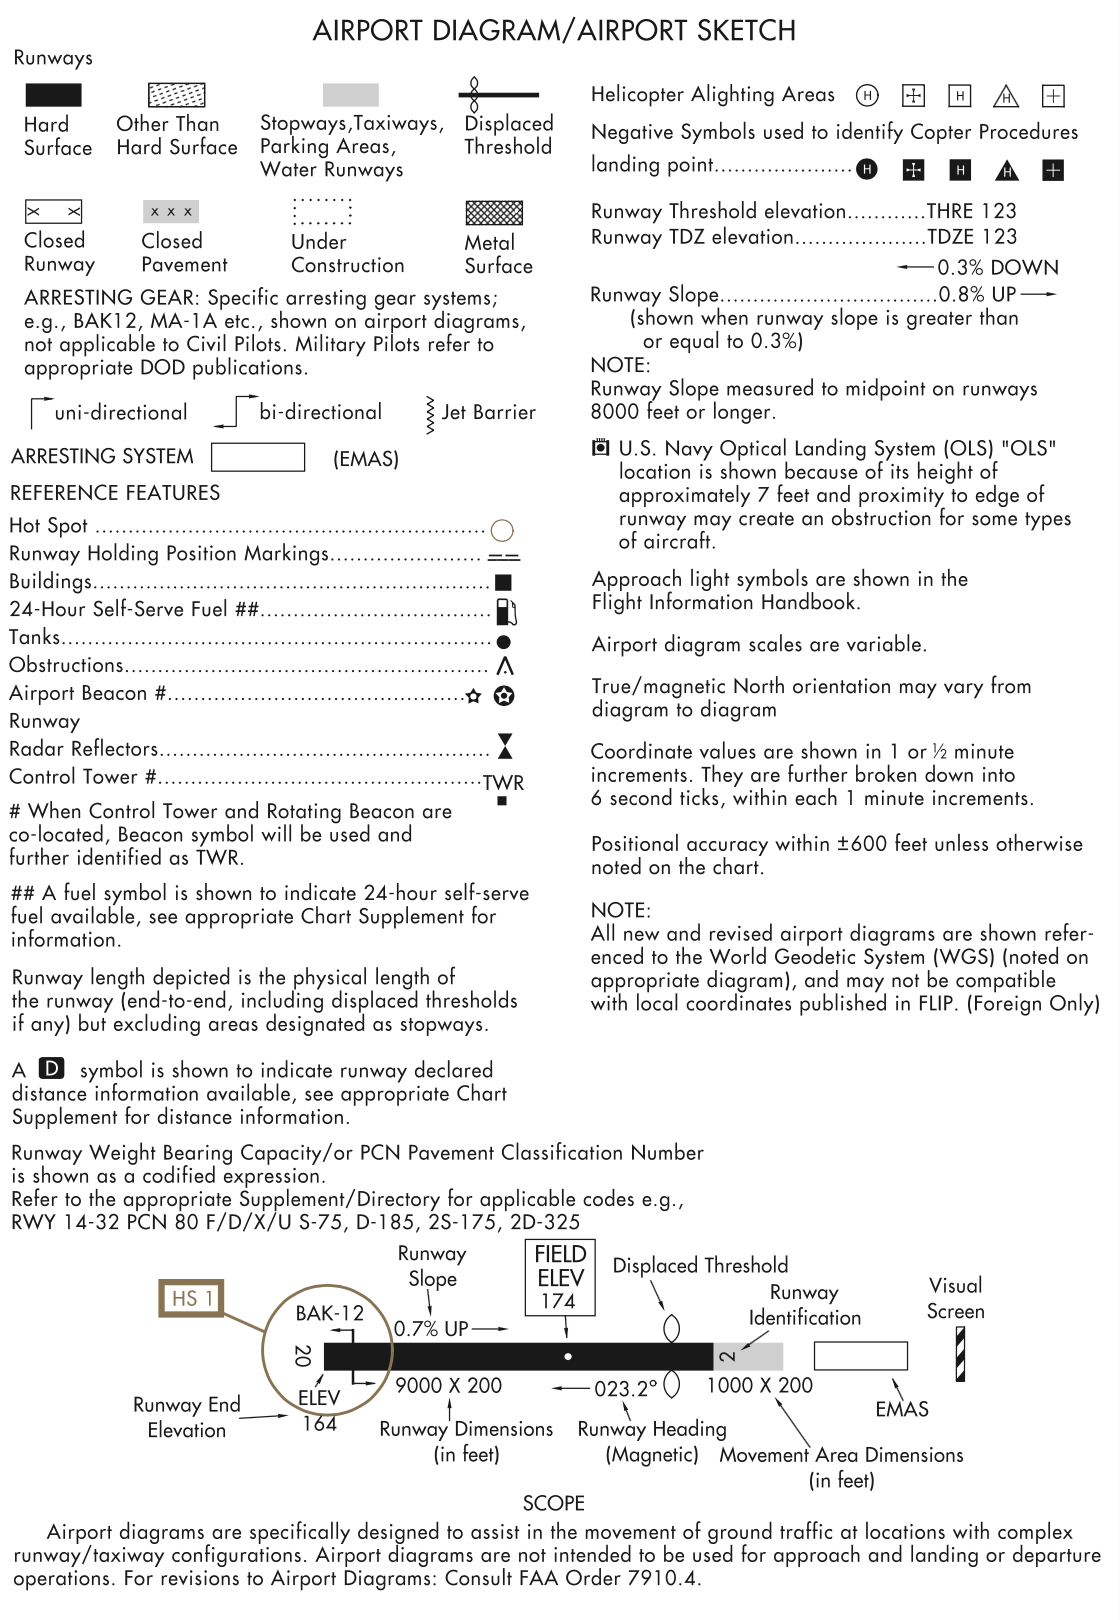
\includegraphics[width=\linewidth]{Airport Diagram Legend.png}
				\end{figure}
				\newpage
			\paragraph{Chart Supplement \& A/FD}
				The Chart Supplement is a document published by the FAA every 56 days providing comprehensive information on airports open to the public. In addition to airport information, the Chart Supplement contains sectional errata, special notices, regulatory notices, airport diagrams, and more.\footnote{\href[page=339]{./phak.pdf}{PHAK - Chart Supplement U.S. (formerly Airport/Facility Directory)}}\\

				The Airport/Facility Directory is a section of the Chart Supplement that contains information on all public use airports in a particular geographic region.\\

				Legend of an A/FD page:\\
				\begingroup
				\fontsize{8pt}{10pt}
				\begin{multicols}{2}
				\begin{enumerate}
					\item City/Airport Name
					\item Alternate Name, if any
					\item Location Identifier
					\item Operating agency, no classification indicates airport is open to public.
					\item Airport location w.r.t the distance and cardinal direction from its associated city.
					\item Time conversion from UTC. All times on an AF/D page are listed in UTC.
					\item Lat/Long coordinates for the approximate geometric centre of all usable runway surfaces.
					\item Charts: the name of the sectional chart, Low and High Enroute charts on which the airport is depicted.
					\item IAP indicates a public use FAA Instrument Approach Procedure. AD indicates a published airport diagram.
					\item A sketch of an airport, useful in absence of am Airport Diagram
					\item Elevation in feet of the highest point of an airport's runways
					\item B indicates a rotating beacon, operating from sunset to sunrise.
					\item Traffic Pattern Altitude or TPA, indicated in MSL(AGL). Mutiple TPA will be shown as "TPA-See Remarks"
					\item AOE - Airport of Entry, no notice for Customs; LRA - Landing Rights Airport, advance notice for Customs.
					\item Certification of airport and vailability of emergency services.
					\item NOTAM file, to refer to for applicable NOTAMs
					\item FAA inspection
					\item Runway data, including: dimensions, materials, slope, lighting, designation, obstacles, and traffic pattern direction.
					\item LAHSO operations and available landing distances
					\item Runway declared distance information
					\item Arresting gear
					\item Available service and times for fuel, oxygen, lighting, etc.
					\item Airport remarks including attendance schedule, and other pertinant information. Information on multiple TPAs will be listed here.
					\item  Millitary Remarks
					\item Airport Manager
					\item Weather Data, frequency and telephone.
					\item Communication frequencies for airport, relavant approach control, center, RCO, and Flight Service Station.
					\item Airspace of airport (includes times if time varying)
					\item VOR Test Facility, if available.
					\item Radio aids to navigation, including nearby VORs, NDBs, and localizer equipment at the airport. Includes class of radio aid: (T) for terminal area, (L) for low altitude, (H) for High Altitude.
					\item Remarks on the availability of radio communications
				\end{enumerate}
				\end{multicols}
				\endgroup
				\begin{figure}
					\centering
					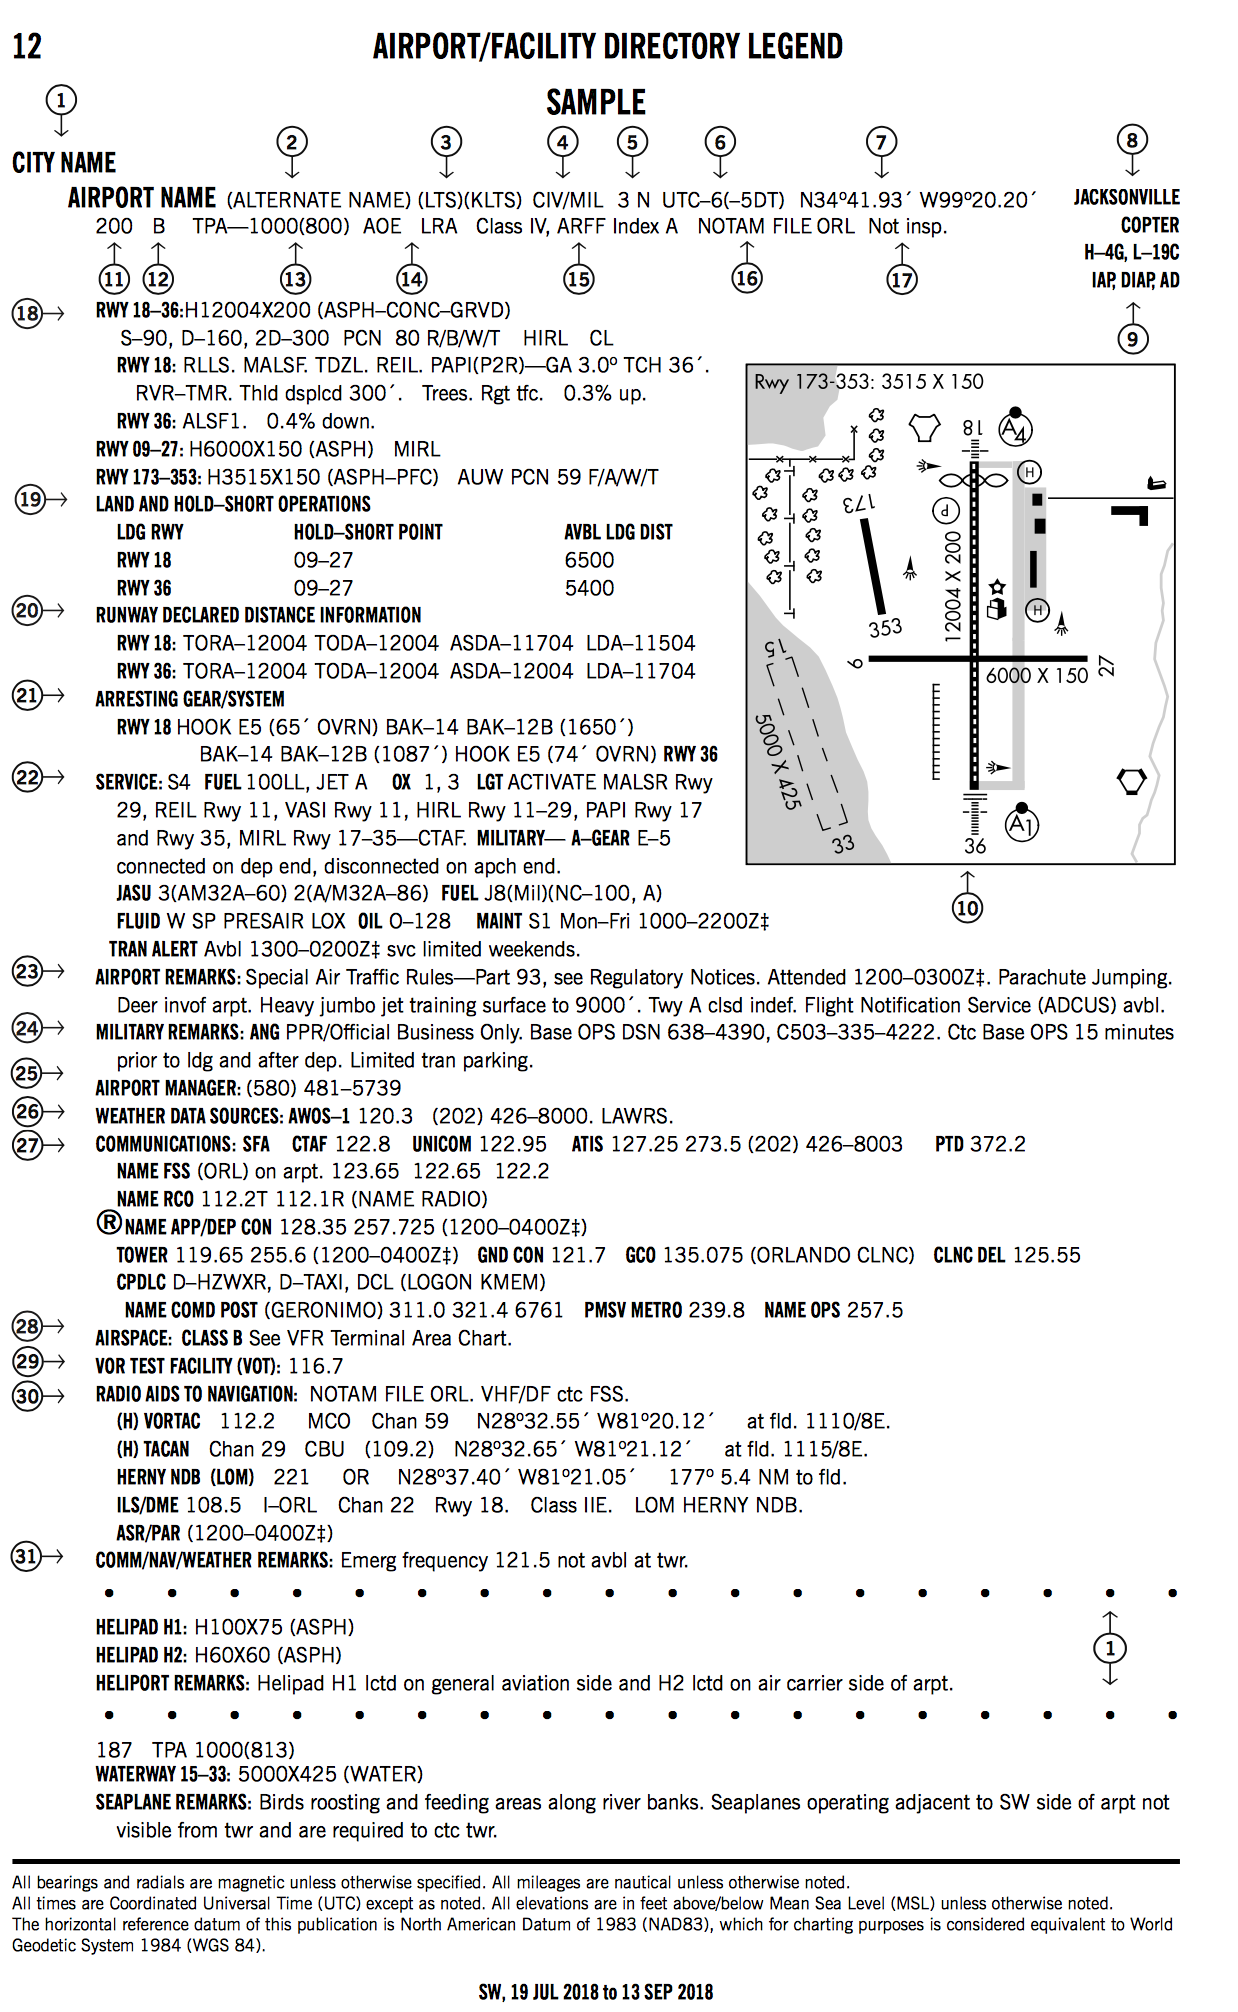
\includegraphics[width=0.55\linewidth]{Figures/AFD Legend.png}
				\end{figure}
				\newpage
			\paragraph{NOTAMs} - Notices to Airmen list time-critical aeronautical information, which is of a temporary nature or not sufficiently known in advance to permit publication, on aeronautical charts. It includes such information as taxiway and runway closures, construction, communications, changes in status of navigational aids, and other information essential to planned en route, terminal, or landing operations. \footnote{\href[page=340]{./phak.pdf}{PHAK - Notices to Airmen (NOTAM)}}
			\paragraph{Sectional Chart}
				\begin{wrapfigure}{l}{0.3\textwidth}
					\centering
					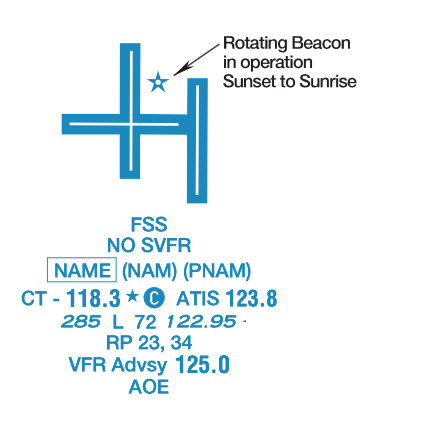
\includegraphics[width=\linewidth]{Figures/Sectional Airport.png}
				\end{wrapfigure}
				Sectional Charts, while primarily used for enroute planning, lists limited information about airports. An airport on a sectional chart is depicted in blue if it is a towered airport, and magenta if it is un-towered. The airport's name, identifier, control tower/ctaf frequency, beacon, ATIS/AWOS, field elevation, controlled lighting, length of its longest runway in 100s of feet, UNICOM frequency, traffic pattern direction and advisory information are listed. Airports with fuel available will be surrounded by tick marks. Airports without paved runways are depicted by an open circle. Private airports are labeled by an encicled R.\\
		\subsubsection{Weather Information - ATIS, AWOS}
			Automated Terminal Information Service (ATIS) is a recording of the local weather conditions and other pertinent non-control information broadcast on a local frequency. It is normally updated once per hour but is updated more often when changing local conditions warrant. Important information is broadcast on ATIS including weather, runways in use, specific ATC procedures, and any airport construction activity that could affect taxi planning. When the ATIS is recorded, it is given a code. This code is changed with every ATIS update. For example, ATIS Alpha is replaced by ATIS Bravo. The next hour, ATIS Charlie is recorded, followed by ATIS Delta and progresses down the alphabet.\footnote{\href[page=341]{./phak.pdf}{PHAK - Automated Terminal Information Service (ATIS)}}\\

			Automated Weather Observing Service(AWOS) is an automated broadcast of weather in the vicinity of the airport. It is typically updated every minute. AWOS data include barometric pressure, altimeter setting, wind speed, gusts and direction; current ceilings and visibility, and more depending on the type of AWOS system installed. 
	\subsection{Surface Operations}
		\subsubsection{Areas of an Airport}
			An airport is divided into several areas:
			\begin{itemize}
				\item Non-movement area: surface areas not under ATC control, unsually but not always demarkated by a solid yellow line and broken yellow line. The solid line is on the side where permission is required to cross from. (e.g ramp)
				\item Taxiways: used for aircraft to move from a ramp/parking area to a runway.
				\item Runways: the surface from threshold to threshold where aircraft are allowed to takeoff and land. Runways are broken up further into the following areas:
				\begin{itemize}
					\item Runway Safety Area: a defined surface surrounding the runway prepared, or suitable, for reducing the risk of damage to airplanes in the event of an undershoot, overshoot, or excursion from the runway.
					\item Runway threshold: the markings across the runway that denote the beginning and end of the runway, a solid white line.
					\item Displaced runway threshold: this area can be used for taxiing, takeoff, rollout, but not for touchdown.
					\item Blast Pads (or overrun areas, or stopways): are constructed before the start of a runway where jetblast is a concern. and may also be used as emergency space for planes to land, taxi, or overrun in case of a rejected takeoff.
				\end{itemize}
				Runways are broken up into the following lengths:
				\begin{itemize}
					\item Takeoff Run Available (TORA): the runway length available for takeoff; from displaced threshold to threshold in the direction of takeoff
					\item Takeoff Distance Available (TODA): TORA plus the length of the clearway
					\item Accelerate-Stop Distance Available (ASDA): TORA plus the length of the stopway if provided for the acceleration and deceleration of an airplane aborting a takeoff
					\item Landing Distance Available (LDA): the runway length available to land; threshold to displaced threshold in the direction of landing.
				\end{itemize}
				\begin{figure}[h]
					\centering
					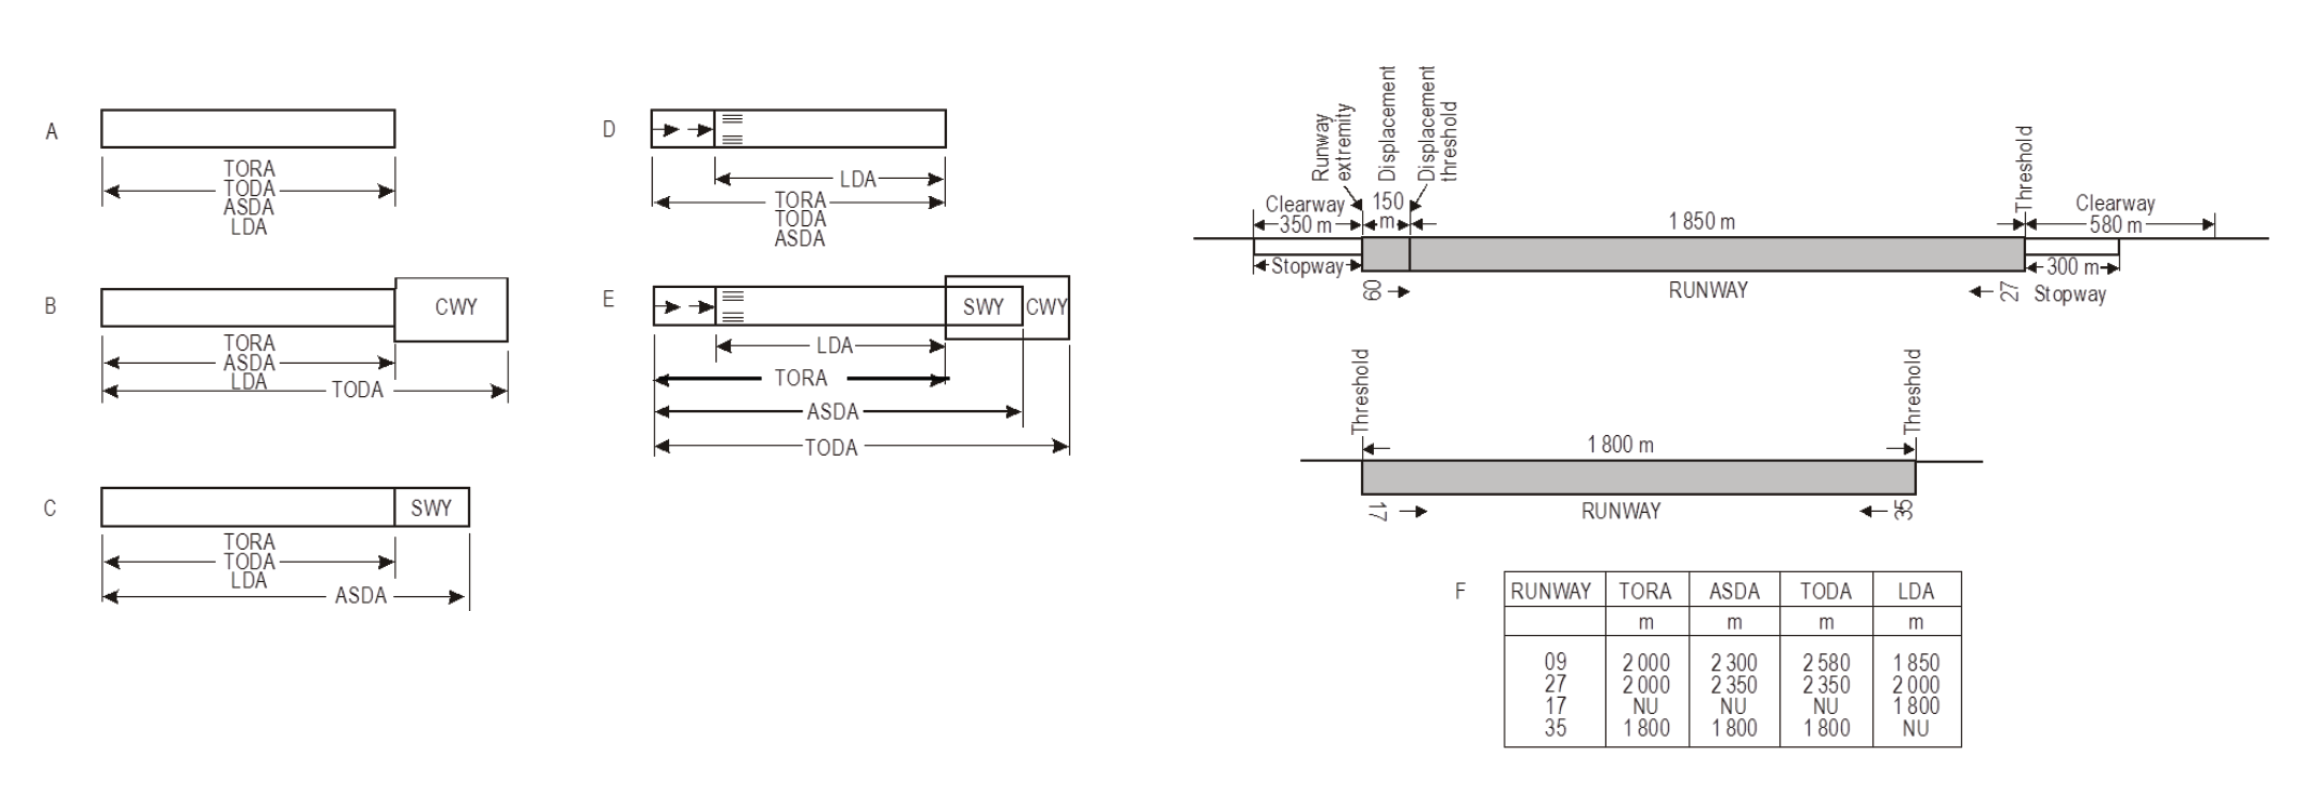
\includegraphics[width=\linewidth]{Figures/Runway Lengths.png}
				\end{figure}
			\end{itemize}
			\newpage
		\subsubsection{Airport Signage, Markings \& Lighting}	\footnote{\href{https://www.faa.gov/airports/runway_safety/publications/media/QuickReferenceGuideProof8.pdf}{FAA - Runway Safety: Airport Sign and Markings Quick Reference Guide}}
			\begin{figure}[h]
				\centering
				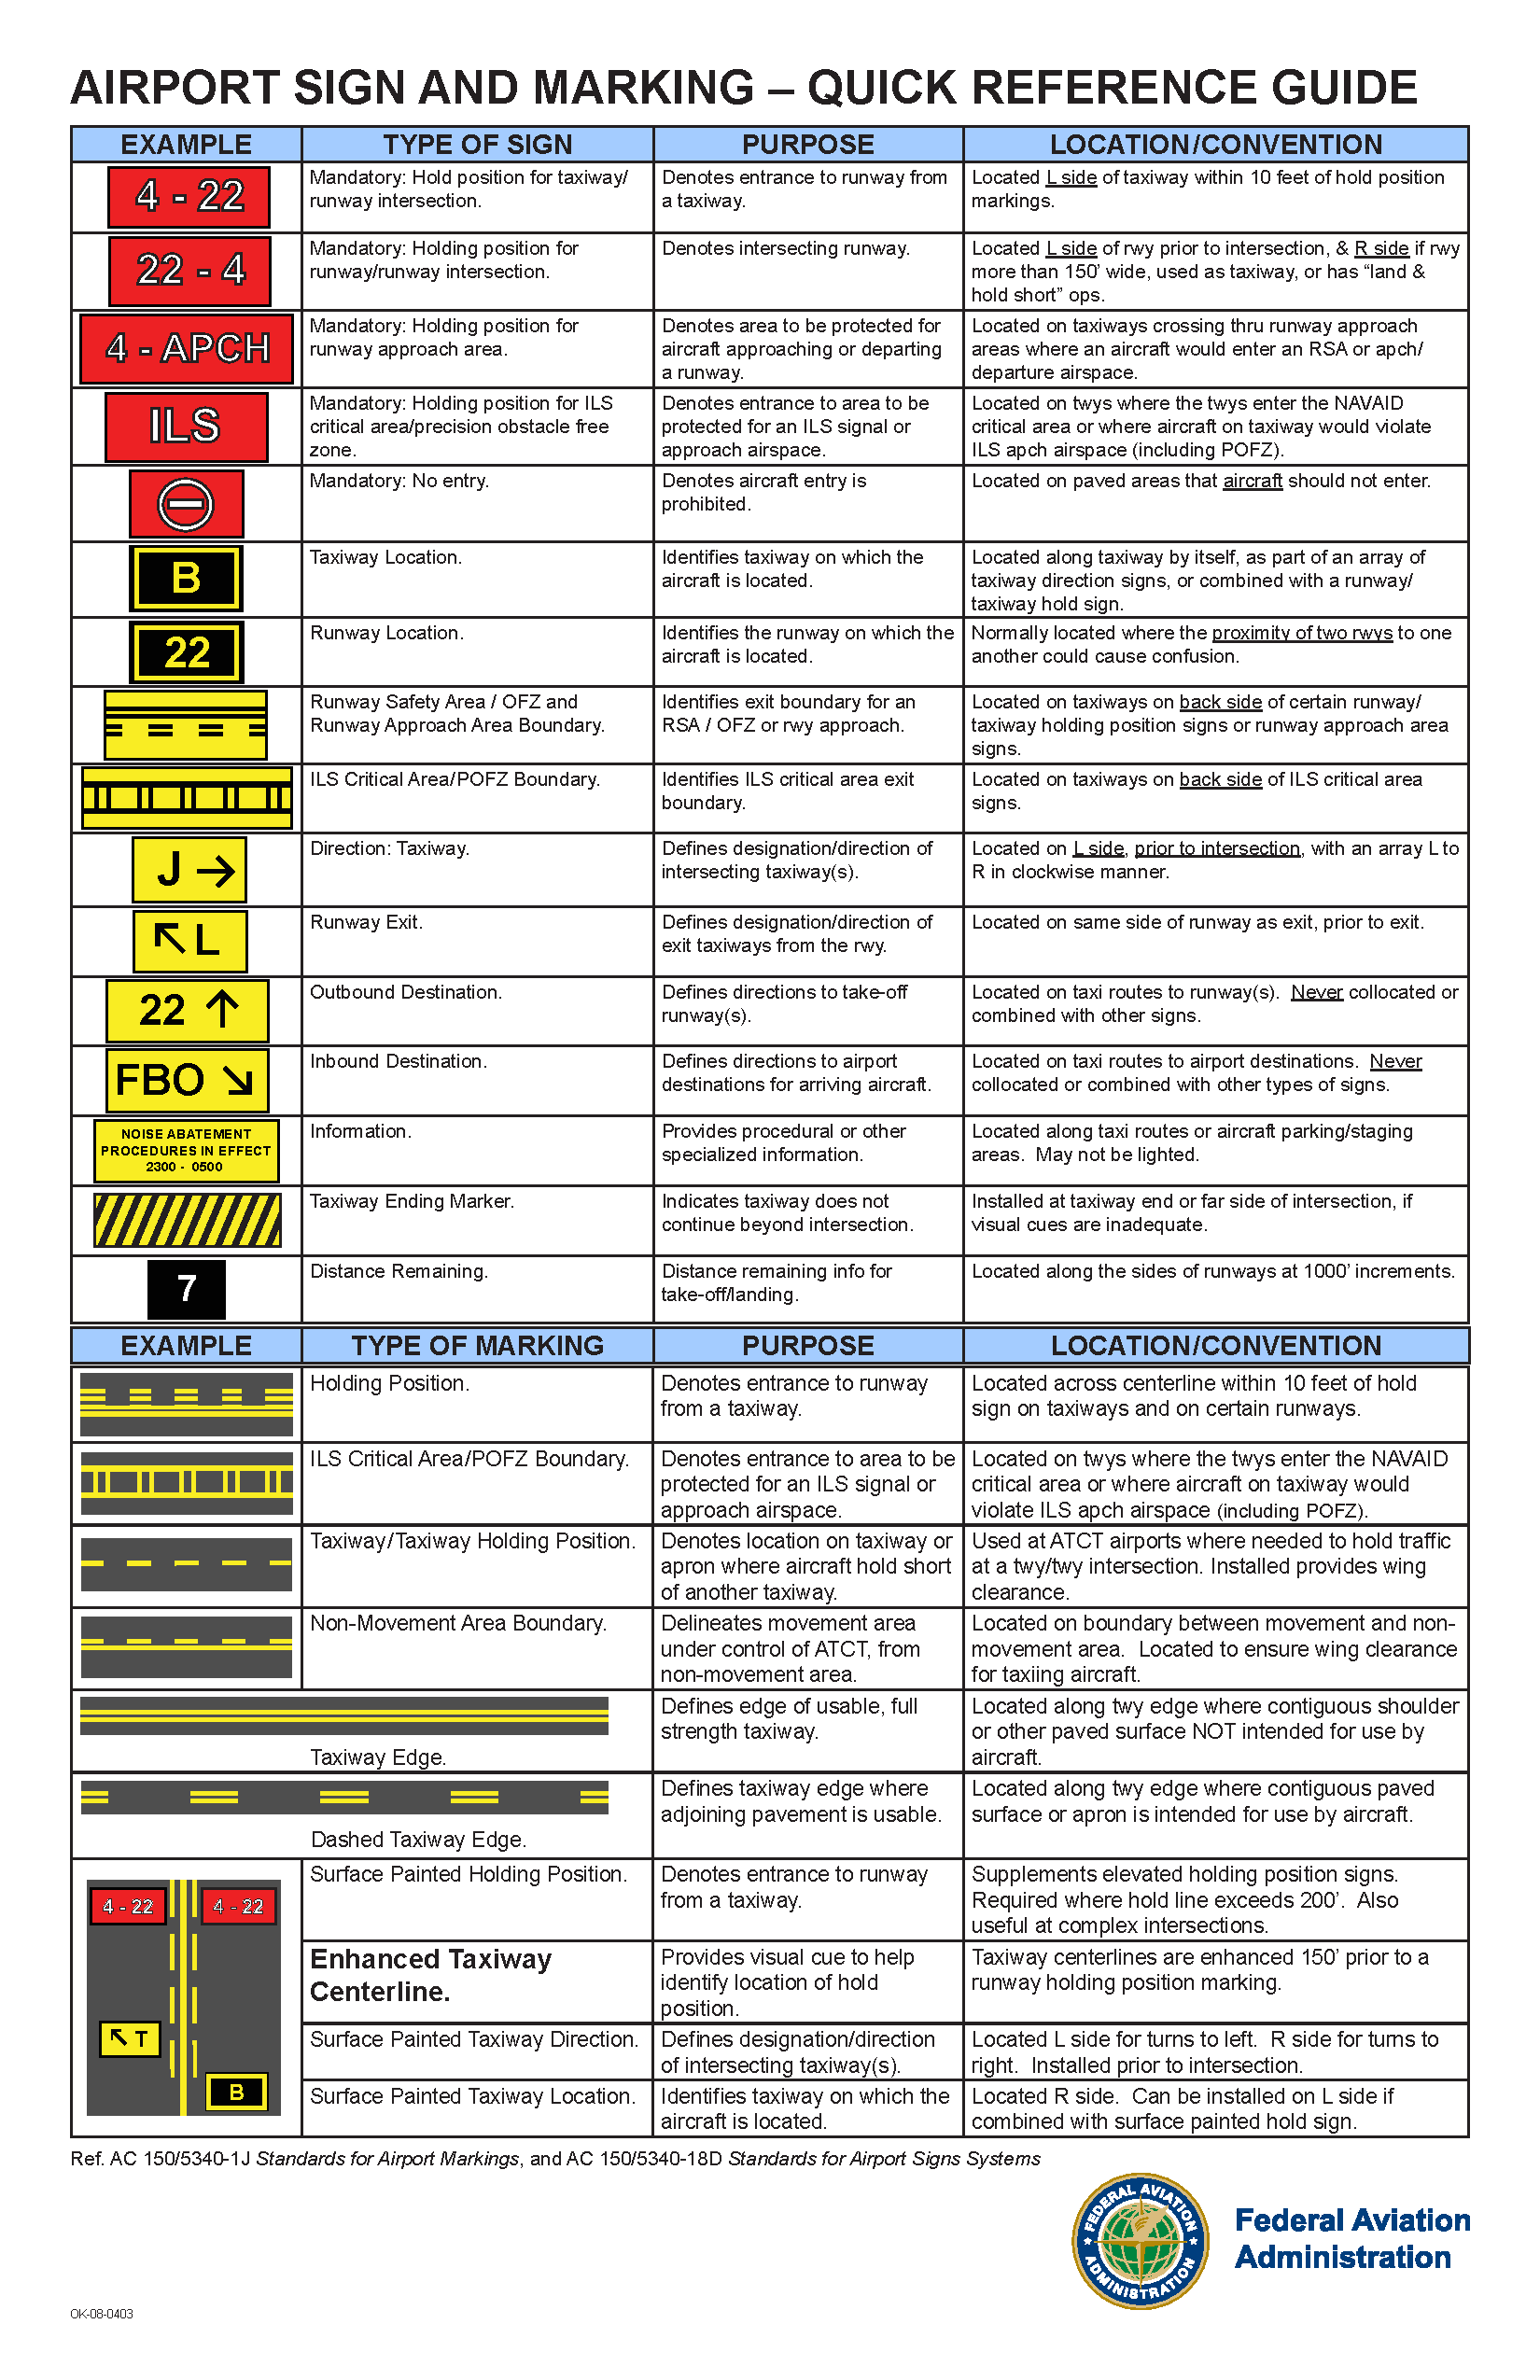
\includepdf[pages=1,pagecommand={},width=0.9\textwidth]{Figures/Airport Markings.pdf}
			\end{figure}
			\newpage
			\paragraph{Airport Markings}
			\begin{itemize}
				\item\textbf{Wind Direction Indicators} Wind indicators, in the absence of weather reporting, inform a pilot of the surface wind conditions at an airport. There are three types of wind direction indicators.
				\begin{enumerate}
					\item Wind Sock: A wind sock, is simply a sock shaped cloth that extends in the direction that the wind is blowing towards (and inflated from the direction the wind is blowing from). The degree to which the wind sock is extended can be used to estimate the wind speed. A fully extended wind sock generally indicates a wind of greater than 15 knots. 
					\item Tetrahedron: A tetrahedron shaped indicator that tapers in the direction that the wind is coming from.
					\item Wind tee: A ``T'' shaped indicator that alligns lengthwise in the direction of wind, with the horizonal bar extending on the upwind side. Pictorally they represent an airplane, and its preferred landing direction.
				\end{enumerate}
				\item\textbf{Segmented Circle} The segmented circle is a visual aid for pilots to determine the direction of an airport traffic pattern, and which runway to land on. It depicts a base and final leg for each runway; the direction of the base to final turn is the direction of the entire traffic pattern. Combined with the wind direction indicators, a pilot can determine the preferred runway(s).
					\begin{figure}[H]
			    		\centering
			    		\subfloat{{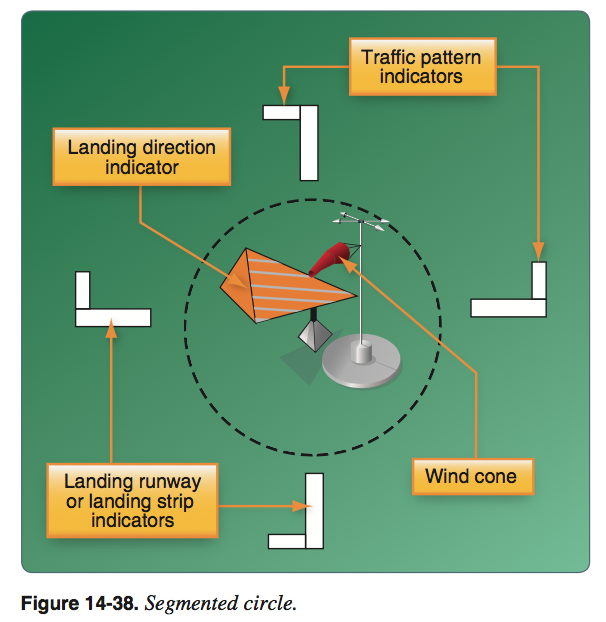
\includegraphics[width=0.3\linewidth]{Figures/Segmented Circle.png}}}
			    		\subfloat{{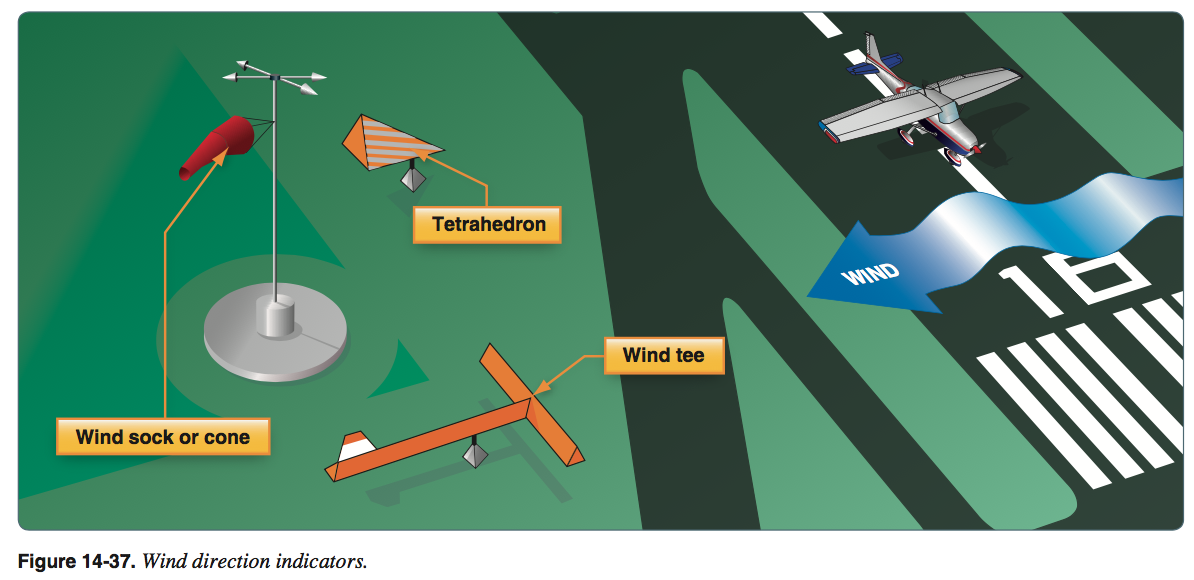
\includegraphics[width=0.7\linewidth]{Figures/Wind Direction Indicators.png}}}
					\end{figure}
				\item\textbf{Runway Markings}\footnote{\href[page=96]{./aim.pdf}{AIM: 2-3-3 Runway Markings}}\\
					There are three types of markings for runways: visual, nonprecision instrument, and precision instrument. Table 2-3-1 summarized which markings are located on which runways, and Figure 2-3-2 illustrates the appearance of these markings.
					\begin{figure}[H]
						\centering
						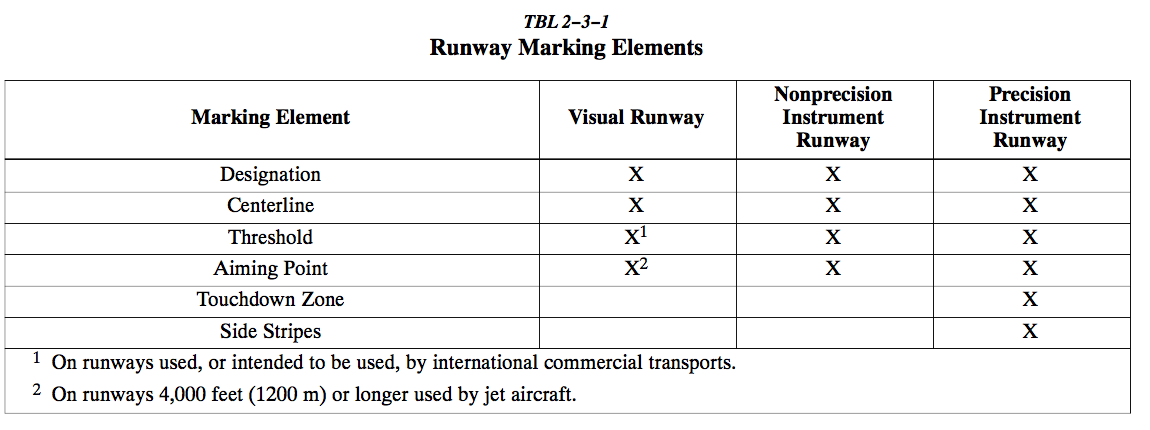
\includegraphics[width=\linewidth]{Figures/Runway Marking Elements.png}
						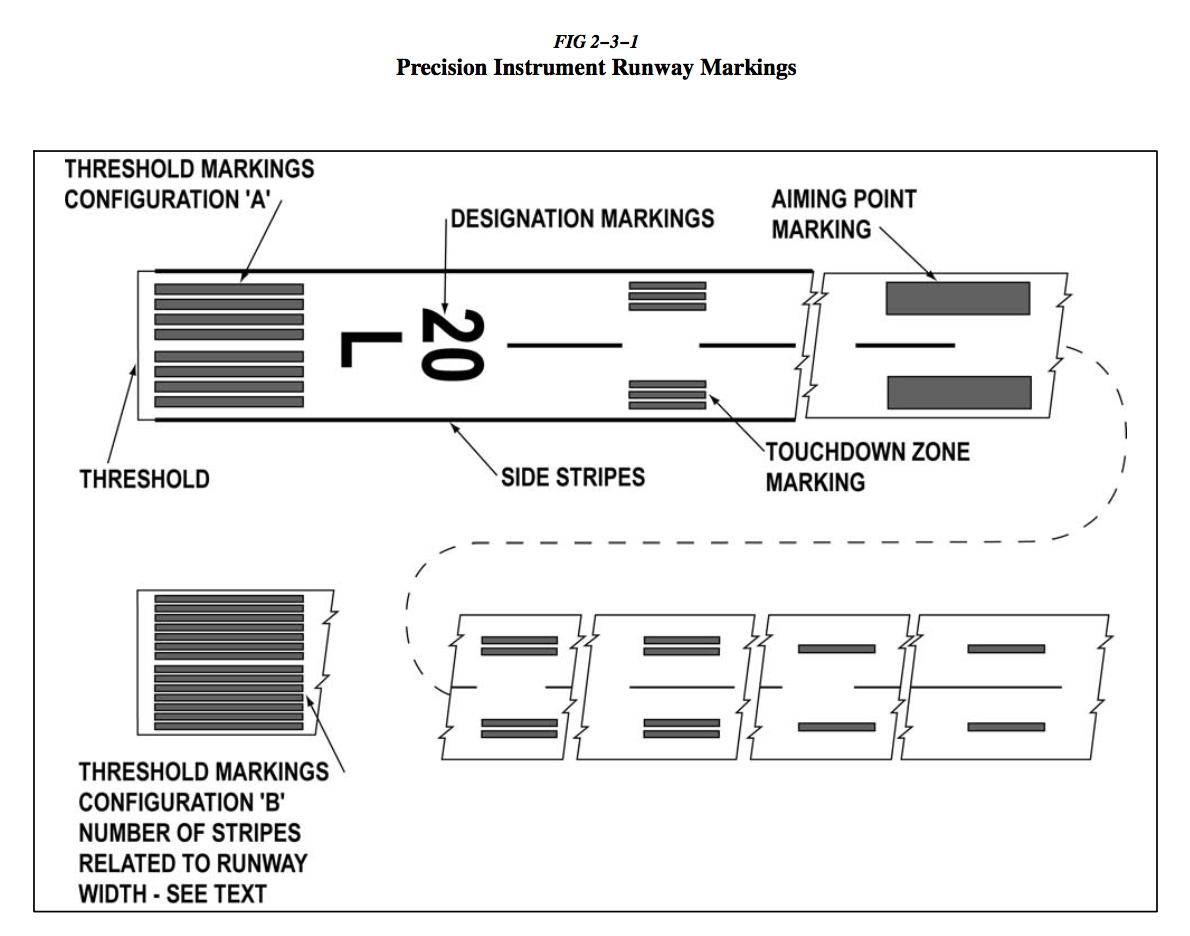
\includegraphics[width=\linewidth]{Figures/Precision Instrument Runway Markings.png}
					\end{figure}
				\begin{enumerate}
					\item Runway Designators: Runway numbers and letters are determined from the approach direction. The runway number is the whole number nearest one-tenth the magnetic azimuth of the centerline of the runway, measured clockwise from the magnetic north. The letters, differentiate between left (L), right (R), or center (C) parallel runways, as applicable.
					\item Runway Centerline Marking: The runway centerline identifies the center of the runway and provides alignment guidance during takeoff and landings. The centerline consists of a line of uniformly spaced stripes and gaps. 
					\item Runway Aiming Point Marking: The aiming point marking serves as a visual aiming point for a landing aircraft. These two rectangular markings consist of a broad white stripe located on each side of the runway centerline and approximately 1,000 feet from the landing threshold.
					\item Runway Touchdown Zone Markers: The touchdown zone markings identify the touchdown zone for landing operations and are coded to provide distance information in 500 feet (150m) increments. These markings consist of groups of one, two, and three rectangular bars symmetrically arranged in pairs about the runway centerline. For runways having touchdown zone markings on both ends, those pairs of markings which extend to within 900 feet (270 m) of the midpoint between the thresholds.
					\item Runway Side Stripe Marking: Runway side stripes delineate the edges of the runway. They provide a visual contrast between runway and the abutting terrain or shoulders. Side stripes consist of continuous white stripes located on each side of the runway.
					\item Runway Shoulder Markings: supplement runway side stripes to identify pavement areas contiguous to the runway sides that are not intended for use by aircraft. Runway shoulder stripes are yellow.
					\item Runway Threshold Markings: a set number of parallel stripes on the runway that indicate the width of a runway.
						\begin{itemize}
							\item 60 feet - 4 stripes
							\item 75 feet - 6 stripes
							\item 100 feet - 8 stripes
							\item 150 feet - 12 stripes
							\item 200 feet 16 stripes
						\end{itemize}
					\item Displaced Threshold: A displaced threshold is indicated by white arrows extending up to the runway threshold.
					\item Demaraction bar: A yellow bar that separates the runway or displaced threshold from a blast pad, stopway, or taxiway.
					\item Chevrons: Yellow chevrons are used to show pavement areas aligned with the runway that are unusable for landing, takeoff, and taxiing.
				\end{enumerate}
			\item\textbf{Taxiway Markings}\footnote{\href[page=101]{./aim.pdf}{AIM: 2-3-4 Taxiway Markings}}:
				All taxiways should have centerline markings and runway holding position markings whenever they intersect a runway. Taxiway edge markings are present whenever there is a need to separate the taxiway from a pavement that is not intended for aircraft use or to delineate the edge of the taxiway. Taxiways may also have shoulder markings and holding position markings for Instrument Landing System (ILS) critical areas and taxiway/ taxiway intersection markings.\\
				\begin{enumerate}
					\item Taxiway Centerline: The taxiway centerline is a single continuous yellow line, 6 inches (15 cm) to 12 inches (30 cm) in width. This provides a visual cue to permit taxiing along a designated path. 
					\item Enhanced Centerline: The enhanced taxiway centerline marking consists of a parallel line of yellow dashes on either side of the normal taxiway centerline. The taxiway centerlines are enhanced for a maximum of 150 feet prior to a runway holding position marking.
					\item Taxiway Edge Markings: Taxiway edge markings are used to define the edge of the taxiway. They are primarily used when the taxiway edge does not correspond with the edge of the pavement. These consist of a continuous double yellow line. Dashed taxiway edge markings consist of a broken double yellow line. These markings are used when there is an operational need to define the edge of a taxiway or taxilane on a paved surface where the adjoining pavement to the taxiway edge is intended for use by aircraft.
				\end{enumerate}
		\end{itemize}

			\paragraph{Airport Beacon}\footnote{\href[page=352]{./phak.pdf}{PHAK - Airport Lighting, Airport Beacon}}
			Airport beacons help a pilot identify an airport at night. The beacons are normally operated from dusk until dawn. Sometimes they are turned on if the ceiling is less than 1,000 feet and/or the ground visibility is less than 3 statute miles (VFR minimums). However, there is no requirement for this, so a pilot has the responsibility of determining if the weather meets VFR requirements. \\
			Some of the most common beacons are:
			\begin{itemize}
				\item Flashing white and green for civilian land airports
				\item Flashing white and yellow for a water airport
				\item Flashing white, yellow, and green for a heliport
				\item Two quick white flashes alternating with a green flash identifying a military airport
			\end{itemize}

			\paragraph{Approach Light System (ALS)}
			ALS provide the basic means to transition from instrument flight to visual flight for landing. Approach lights can also aid pilots operating under VFR at night.\footnote{\href[page=352]{./phak.pdf}{PHAK - Airport Lighting, Approach Light Systems}}\footnote{\href[page=77]{./aim.pdf}{AIM: 2-1-1 Approach Light Systems (ALS)}}
			\paragraph{Visual Glideslope Indicators}
			Visual glideslope indicators provide the pilot with glidepath information that can be used for day or night approaches. By maintaining the proper glidepath as provided by the system, a pilot should have adequate obstacle clearance and should touch down within a specified portion of the runway.\footnote{\href[page=352]{./phak.pdf}{PHAK - Airport Lighting, Visual Glideslope Indicators}}\\
			

			\begin{itemize}
				\item \textbf{Visual Approach Slope Indicator (VASI)} VASI installations are the most common visual glidepath systems in use. The VASI provides obstruction clearance within $10^\circ$ of the extended runway centerline and up to 4 nmi from the runway threshold. The VASI consists of light units arranged in bars. There are 2-bar and 3-bar V ASIs. The 2-bar VASI has near and far light bars and the 3-bar VASI has near, middle, and far light bars. Two-bar VASI installations provide one visual glidepath that is normally set at $3^\circ$. The 3-bar system provides 	two glidepaths, the lower glidepath normally set at $3^\circ$ and the upper glidepath 1⁄4 degree above the lower glidepath.
				\item \textbf{Precision Approach Path Indicator (PAPI)} PAPIs  use lights similar to the V ASI system, except they are installed in a single row, normally on the left side of the runway.
			\end{itemize}
				\begin{figure}[H]
				    \centering
				    \subfloat{{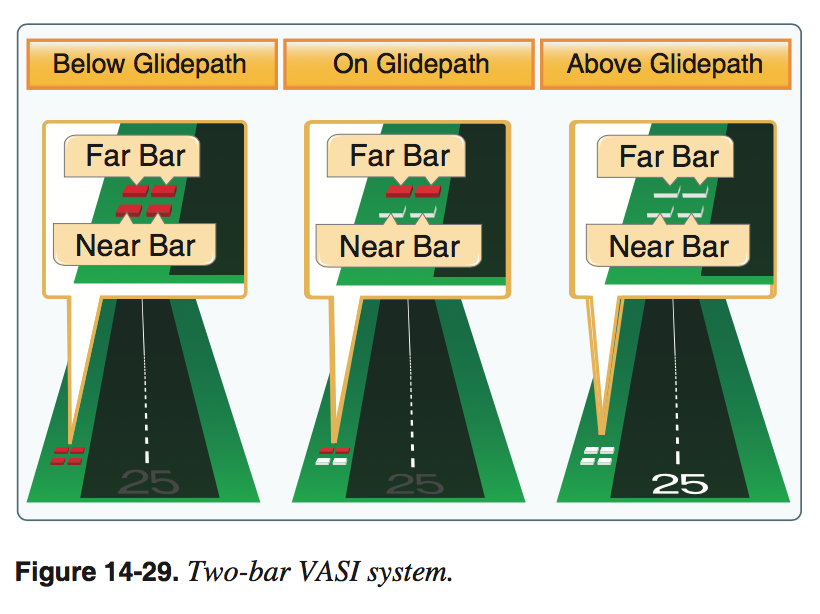
\includegraphics[width=0.3\linewidth]{Figures/VASI.png}}}
				    \subfloat{{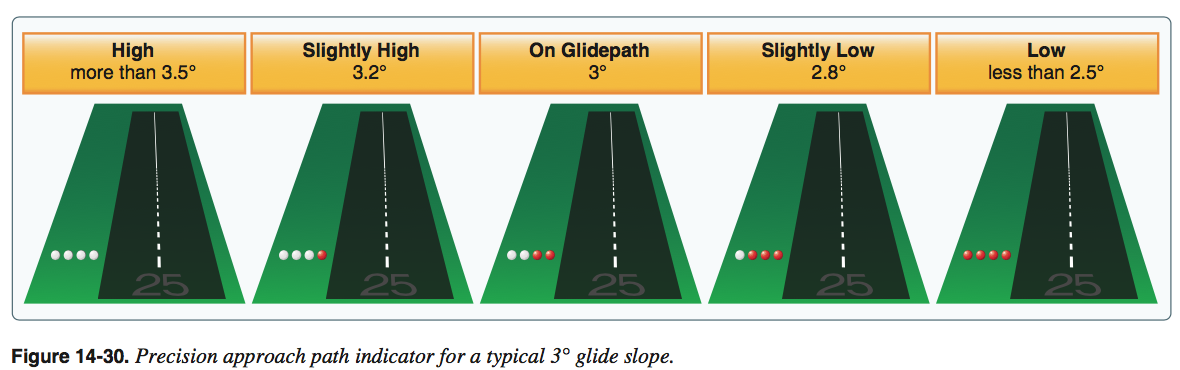
\includegraphics[width=0.7\linewidth]{Figures/PAPI.png}}}
				\end{figure}

			\paragraph{Surface Lighting}
				Airport surfaces are illuminated for night-time and low visibility operations.
			\begin{itemize}
				\item\textbf{Runway Lighting:}
				\begin{itemize}
					\item Runway End Identifier Lights (REIL): The system consists of a pair of synchronized flashing (white) lights located laterally on each side of the runway threshold. REILs may be either omnidirectional or unidirectional facing the approach area. \footnote{\href[page=82]{./aim.pdf}{AIM: 2-1-3 Runway End Identifier Lights (REIL)}}
					\item Runway Edge Light Systems: they come in three intensities (High Intensity Runway Lights(HIRL), Medium (MIRL), Low (LIRL)). The runway edge lights are white, except on instrument runways yellow replaces white on the last 2,000 feet or half the runway length, whichever is less, to form a caution zone for landings. The lights marking the ends of the runway emit red light toward the runway to indicate the end of runway to a departing aircraft and emit green outward from the runway end to indicate the threshold to landing aircraft. \footnote{\href[page=82]{./aim.pdf}{AIM: 2-1-4 Runway Edge Light Systems}}
					\item In-runway Lighting \footnote{\href[page=82]{./aim.pdf}{AIM: 2-1-5 In−runway Lighting}}
						\begin{itemize}
							\item Runway Centerline Lighting System (RCLS): They are located along the runway centerline and are spaced at 50 foot intervals. When viewed from the landing threshold, the runway centerline lights are white until the last 3,000 feet of the runway. The white lights begin to alternate with red for the next 2,000 feet, and for the last 1,000 feet of the runway, all centerline lights are red.
							\item Touchdown Zone Lights (TDZL): They consist of two rows of transverse light bars disposed symmetrically about the runway centerline. The system consists of steady−burning white lights which start 100 feet beyond the landing threshold and extend to 3,000 feet beyond the landing threshold or to the midpoint of the runway, whichever is less.
							\item Taxiway Centerline Lead-Off Lights: Alternate green and yellow lights are installed, beginning with green, from the runway centerline to one centerline light position beyond the runway holding position or ILS critical area holding position.
							\item Taxiway Centerline Lead-On Lights: Taxiway centerline lead−on lights provide visual guidance to persons entering the runway.
							\item Land and Hold Short Lights: Land and hold short lights are used to indicate the hold short point on certain runways which are approved for Land and Hold Short Operations (LAHSO). Land and hold short lights consist of a row of pulsing white lights installed across the runway at the hold short point. Where installed, the lights will be on anytime LAHSO is in effect. 
						\end{itemize}
				\end{itemize}
				\item\textbf{Taxiway Lights:}\footnote{\href[page=91]{./aim.pdf}{AIM: 2-1-11 Taxiway Lights}}\\
					\begin{itemize}
						\item Taxiway Edge Lights: Taxiway edge lights are used to outline the edges of taxiways during periods of darkness or restricted visibility conditions. These fixtures emit blue light.
						\item Taxiway Centerline Lights: they are located along the taxiway centerline, and along designated taxiing paths in portions of runways, ramp, and apron areas. Taxiway centerline lights are steady burning and emit green light.
						\item Clearance Bar Lights: Clearance bar lights are installed at holding positions on taxiways in order to increase the conspicuity of the holding position in low visibility conditions. They may also be installed to indicate the location of an intersecting taxiway during periods of darkness. Clearance bars consist of three in−pavement steady−burning yellow lights.
						\item Runway Guard Lights. Runway guard lights are installed at taxiway/runway intersections. They are primarily used to enhance the conspicuity of taxiway/runway intersections during low visibility conditions, but may be used in all weather conditions. Runway guard lights consist of either a pair of elevated flashing yellow lights installed on either side of the taxiway, or a row of in−pavement yellow lights installed across the entire taxiway, at the runway holding position marking.
						\item Stop Bar Lights. Stop bar lights, when installed, are used to confirm the ATC clearance to enter or cross the active runway in low visibility conditions (below 1,200 ft Runway Visual Range). A stop bar consists of a row of red, unidirectional, steady−burning in−pavement lights installed across the entire taxiway at the runway holding position, and elevated steady−burning red lights on each side. A controlled stop bar is operated in conjunction with the taxiway centerline lead−on lights which extend from the stop bar toward the runway. Following the ATC clearance to proceed, the stop bar is turned off and the lead−on lights are turned on. Pilots should never cross a red illuminated stop bar, even if an ATC clearance has been given to proceed onto or across the runway.
					\end{itemize}
			\end{itemize}
			\paragraph{Pilot Controlled Lighting}
					\begin{wrapfigure}{lh}{0.5\textwidth}
						\centering
						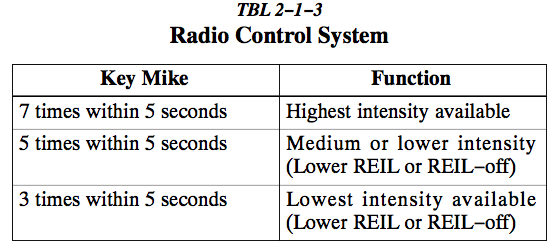
\includegraphics[width=\linewidth]{Figures/PCL.png}
					\end{wrapfigure}
				Operation of approach light systems and runway lighting is controlled by the control tower. At some locations the FSS may control the lights where there is no control tower in operation.\footnote{\href[page=87]{./aim.pdf}{AIM: 2-1-8 Control of Lighting Systems}}. Radio control of lighting is available at selected airports to provide airborne control of lights by keying the aircraft’s microphone. Control of lighting systems is often available at locations without specified hours for lighting.

			\paragraph{Obstruction Lighting}
				Obstructions hazardous to flight should be marked/lighted to warn pilots, but many are not. Not all hazards are lit or charted, and are best mitigated by avoiding flight at low altitudes in low visibility.\footnote{\href[page=94]{./aim.pdf}{AIM: 2-2-3 Obstruction Lights}}\\
				Types of lighting:
				\begin{itemize}
					\item Aviation Red Obstruction Lights: Flashing aviation red beacons (20 to 40 flashes per minute) and steady burning aviation red lights during nighttime operation. Aviation orange and white paint is used for daytime marking.\\
					\item Medium Intensity Flashing White Obstruction Lights: Medium intensity flashing white obstruction lights may be used during daytime and twilight with automatically selected reduced intensity for nighttime operation. When this system is used on structures 500 feet (153m) AGL or less in height, other methods of marking and lighting the structure may be omitted. Aviation orange and white paint is always required for daytime marking on structures exceeding 500 feet (153m) AGL. This system is not normally installed on structures less than 200 feet (61m) AGL.
					\item High Intensity White Obstruction Lights: Flashing high intensity white lights during daytime with reduced intensity for twilight and nighttime operation. When this type system is used, the marking of structures with red obstruction lights and aviation orange and white paint may be omitted.
					\item Dual Lighting: A combination of flashing aviation red beacons and steady burning aviation red lights for nighttime operation and flashing high intensity white lights for daytime operation. Aviation orange and white paint may be omitted.
					\item Catenary Lighting. Lighted markers are available for increased night conspicuity of high-voltage transmission line catenary wires.
				\end{itemize}
			\subsubsection{Communication \& Light Gun Signals}
				At a towered airport, there are generally two ATC facilities that manage movement at the airport; ground which manages aircraft movement between parking areas and runways, and tower which manages aircraft movement on runways, when entering, exiting, or crossing runways. Ground will issue taxi instructions from a parking area to a runway. Tower is the facility that will issue a takeoff or landing clearance and instructions to enter and exit runways. In the event of a communications failure the following light gun signals are used\footnote{\href[page=199]{./aim.pdf}{AIM: Table 4-3-11 Airport Traffic Control Tower Light Gun Signals}}:
					\begin{figure}[h]
						\centering
						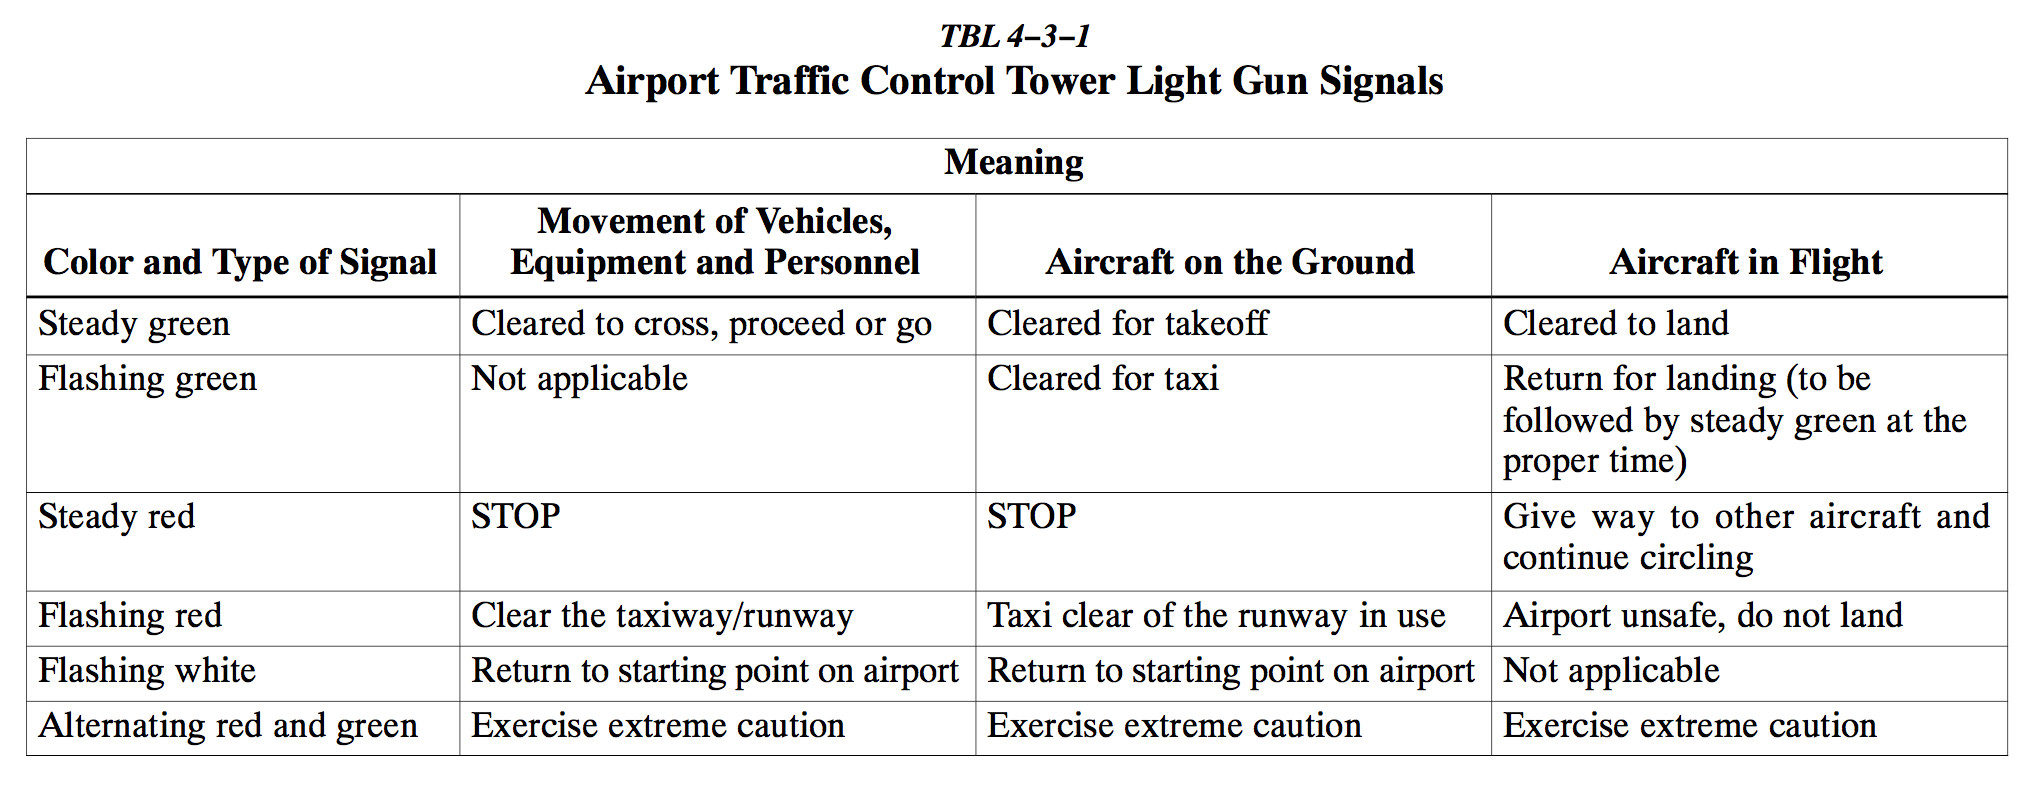
\includegraphics[width=\linewidth]{Figures/Light Gun Signals.png}
						\caption{AIM 4-3-1 Airport Traffic Control Tower Light Gun Signals}
					\end{figure}
			\subsubsection{Taxi Operations}
				Taxi instructions are issued at towered airports to guide planes around an airport. All taxi instructions must be readback with an aircraft's full callsign. Having an airport diagram handy can assist in understanding taxi instructions. A pilot can request ``progressive taxi'' for turn by turn instructions at an unfamiliar airfield.\\

				Approval must be obtained prior to moving an aircraft or vehicle onto the movement area during the hours an Airport Traffic Control Tower is in operation.\footnote{\href[page=202]{./aim.pdf}{AIM: 4-3-18 Taxiing}}
					\begin{enumerate}
						\item Always state your position on the airport when calling the tower for taxi instructions.
						\item The movement area is normally described in local bulletins issued by the airport manager or control tower.
						\item The control tower also issues bulletins describing areas where they cannot provide ATC service due to nonvisibility or other reasons.
						\item A clearance must be obtained prior to taxiing on a runway, taking off, or landing during the hours an Airport Traffic Control Tower is in operation.
						\item A clearance must be obtained prior to crossing any runway. ATC will issue an explicit clearance for all runway crossings.
						\item When assigned a takeoff runway, ATC will first specify the runway, issue taxi instructions, and state any hold short instructions or runway crossing clearances if the taxi route will cross a runway. This does not authorize the aircraft to ``enter'' or ``cross'' the assigned departure runway at any point. In order to preclude misunderstandings in radio communica- tions, ATC will not use the word “cleared” in conjunction with authorization for aircraft to taxi.
						\item When issuing taxi instructions to any point other than an assigned takeoff runway, ATC will specify the point to taxi to, issue taxi instructions, and state any hold short instructions or runway crossing clearances if the taxi route will cross a runway.
						\item If a pilot is expected to hold short of a runway approach (“APPCH”) area or ILS holding position, ATC will issue instructions.
						\item When taxi instructions are received from the controller, pilots should always read back:
						\begin{enumerate}
							\item The runway assignment.
							\item Any clearance to enter a specific runway.
							\item Any instruction to hold short of a specific runway or line up and wait.
						\end{enumerate}
					\end{enumerate}

				The following examples cover radio communication w.r.t Taxi procedures:
				\begin{enumerate}
					\item \textbf{Request for taxi instructions prior to departure}: State your aircraft identification, loca- tion, type of operation planned (VFR or IFR), and the point of first intended landing. \\
					Example: Washington ground, Beechcraft One Three One Five Niner at hangar eight, ready to taxi, I−F−R to Chicago\\
					\item \textbf{Request for taxi instructions after landing.} State your aircraft identification, location, and that you request taxi instructions.\\
					Example: Orlando ground, Beechcraft One Four Two Six One clearing runway one eight left at taxiway bravo three, request taxi to Page.
				\end{enumerate}

					Pilots of departing aircraft should communicate with the control tower on the appropriate ground control/clearance delivery frequency prior to starting engines to receive engine start time, taxi and/or clearance information. A controller may omit the ground or local control frequency if the controller believes the pilot knows which frequency is in use. If the ground control frequency is in the 121 MHz bandwidth the controller may omit the numbers preceding the decimal point; e.g., 121.7, ``CONTACT GROUND POINT SEVEN.'' \footnote{\href[page=199]{./aim.pdf}{AIM: 4-3-14 Communications}}\\

					When conducting taxi operations, pilots need to be aware of their proximity to other aircraft and vehicles moving on the airport. This SA is comprised of, but not limited to, knowledge of the aircraft’s precise position. Pilots should use a ``continuous loop'' process to actively monitor and update their progress and location during taxi. This includes knowing the aircraft’s present location and mentally calculating the next location on the route that will require increased attention (e.g., a turn onto another taxiway, an intersecting runway, or hot spots). SA is enhanced by understanding the ATC clearance issued to the pilots, other aircraft, and vehicles in order to avoid potential conflicts. The following are specific pilot actions to mitigate the pilot causing a runway incursion:\footnote{\href[page=5]{"Refrences/AC 91-73B.pdf"}{AC 91-73B: Parts 91 and 135 Single Pilot, Flight School Procedures During Taxi Operations}}
					\begin{enumerate}
						\item Have a current airport diagram readily available for reference and check the assigned taxi route against the diagram. Tthe pilot(s) must follow the aircraft’s progress on the airport diagram.
						\item Pilot(s) must monitor the taxi clearance and read back all hold short instructions. Verbalizing hold short instructions is a method to ensure that the pilot(s) have a clear understanding of the intended taxi plan and do not cross any runway hold short lines without ATC clearance. 
						\item Know and use all of the visual aids available at the airport, such as the signs, markings, and lighting, as well as ground and/or tower ATC, to follow the taxi route.
						\item Prior to entering or crossing any runway, the pilot must be positive that ATC has cleared them to enter or cross the runway. Pilots should scan the full length of the runway and also scan for aircraft on final approach. If there is any confusion, the pilot should stop and ask ATC to clarify the situation. 
						\item  When approaching an entrance to a runway, pilot(s) will ensure compliance with hold short or crossing clearance. Furthermore, bring the aircraft to a complete stop, or be in a phase of taxiing that has no risk of causing a runway incursion, before continuing with operational duties and checklists. 
						\item Be especially vigilant if another aircraft that has a similar call sign is on frequency. 
						\item If the pilot becomes disoriented, never stop on a runway and initiate communications with ATC to regain orientation.
						\item Pilots should use caution after landing on a runway that intersects another runway, or on a runway where the exit taxiway is in close proximity to another runway’s hold short line.
						\item After landing, ensure that the entire aircraft, including the tail section, has crossed over the respective landing runway’s hold short line.
						\item After landing at a non-towered airport, or at an airport where the control tower is closed, remember that not all aircraft are radio-equipped; therefore, before entering or crossing a runway, listen on the appropriate frequency (common traffic advisory frequency (CTAF)) for inbound aircraft information. Scan the full length of the runway, including the final approach and departure paths of the runway(s) you intend to enter or cross. 
						\item  After landing, nonessential communications and nonessential pilot actions should not be initiated until clear of all runways (e.g., changing radio frequencies and repositioning flaps, and trim).
						\item During landing, do not accept last-minute ATC turnoff instructions unless you clearly understand the instructions and are certain that you can safely comply. 
					\end{enumerate}
					\paragraph{Taxi Technique}
					When taxiing with a quartering headwind, the wing on the upwind side (the side that the wind is coming from) tends to be lifted by the wind unless the aileron control is held in that direction (upwind aileron UP). Moving the aileron into the UP position reduces the effect of the wind striking that wing, thus reducing the lifting action. This control movement also causes the downwind aileron to be placed in the DOWN position, thus a small amount of lift and drag on the downwind wing, further reducing the tendency of the upwind wing to rise.\\
					When taxiing with a quartering tailwind, the elevator should be held in the DOWN position, and the upwind aileron, DOWN. Since the wind is striking the airplane from behind, these control positions reduce the tendency of the wind to get under the tail and the wing and to nose the airplane over. The application of these crosswind taxi corrections helps to minimize the weathervaning tendency and ultimately results in making the airplane easier to steer.\footnote{\href[page=46]{./afh.pdf}{AFH: Ground Operations - Taxiing}}

			\subsubsection{LAHSO Operations}
				Land and Hold Short Operations refer to operations include landing and holding short of an intersecting runway, an intersecting taxiway, or some other designated point on a runway other than an intersecting runway or taxiway. \footnote{\href[page=195]{./aim.pdf}{AIM 4-3-11(a)}}
				Pilots may accept such a clearance provided that the pilot−in−command determines that the aircraft can safely land and stop within the Available Landing Distance (ALD). ALD data are published in the special notices section of the Chart Supplement U.S. and in the U.S. Terminal Procedures Publications. Controllers will also provide ALD data upon request. Student pilots or pilots not familiar with LAHSO should not participate in the program. The pilot−in−command has the final authori- ty to accept or decline any land and hold short clearance. The safety and operation of the aircraft remain the responsibility of the pilot. Pilots are expected to decline a LAHSO clearance if they determine it will compromise safety. Informing oneself of LAHSO operations and pertinent runway lengths should be part of a pilot's preflight. \footnote{\href[page=195]{./aim.pdf}{AIM: 4-3-11(b) Pilot Responsibilities When Conducting Land and Hold Short Operations (LAHSO)}}
			\subsubsection{Runway Incursions}
				A runway incursion occurs whenever an aircraft enters a runway it is not authorized to, which is most critical when another aircraft is landing or taking off, as collisions can occur. Common areas of runway incursion are often denoted on Airport Diagarams as hotspots, circled in beige on FAA charts and red on Jeppesen charts.
			\subsubsection{Line up and wait (LUAW)}
				Line up and wait is an air traffic control (ATC) procedure designed to position an aircraft onto the runway for an imminent departure. The ATC instruction “LINE UP AND WAIT” is used to instruct a pilot to taxi onto the departure runway and line up and wait.\footnote{\href[page=294]{./aim.pdf}{AIM: 5-2-4 Line Up and Wait (LUAW)}} If a takeoff clearance is not received within 90 seconds after clearance to line up and wait, ATC should be contacted. Pilots should be especially vigilant when instructed to taxi and ``Line Up and Wait'' (LUAW). Traffic Collision Avoidance Systems (TCAS)/traffic advisory systems (TAS) should be turned on in order to obtain an awareness of any aircraft that may be landing on their runway. When taxiing onto a runway either at the end of the runway or at an intersection, scan the full length of the runway and scan for aircraft on final approach or landing rollout. \footnote{\href[page=6]{Refrences/AC 91-73B.pdf}{AC 91-73B: Parts 91 and 135 Single Pilot, Flight School Procedures During Taxi Operations}}

	\subsection{Airport Traffic Pattern Operations}
		\subsubsection{Airport Traffic Pattern}
			To assure that air traffic flows into and out of an airport in an orderly manner, an airport traffic pattern is established based on the local conditions, to include the direction and altitude of the pattern and the procedures for entering and leaving the pattern. Unless the airport displays approved visual markings indicating that turns should be made to the right, the pilot should make all turns in the pattern to the left. At most airports traffic pattens are flown at 1000 AGL (Traffic Pattern Altitude(TPA)) , but this altitude may vary both by airport and type of aircraft. An airport's entry in the Chart Supplement will indicate TPA for a given airport. \\

			There are 6 legs in a traffic pattern. All legs are referenced by their associated runway and the direction of turns (except for final and departure which have no directionality)\footnote{\href[page=182]{./aim.pdf}{AIM: 4-3-2 Airports with an Operating Control Tower}}:
			\begin{enumerate}
				\item Departure: the leg extending in the direction of take off away from the referenced runway.
				\item Crosswind: the leg extending perpedicular away from the referenced runway.
				\item Downwind: the leg parallel to the referenced runway, extending in the opposite direction from the direction of takeoff/landing
				\item Base: the leg perpendicular towards the referenced runway.
				\item Final: the leg extending in the direction of landing towards the referenced runway.
				\item Upwind: the leg parallel to the referenced runway, extending in the same direction as the direction of takeoff/landing, offset either left or right. Directions are referenced by the side of the runway where the upwind leg is flown.
			\end{enumerate}

			\begin{figure}[H]
				\centering
				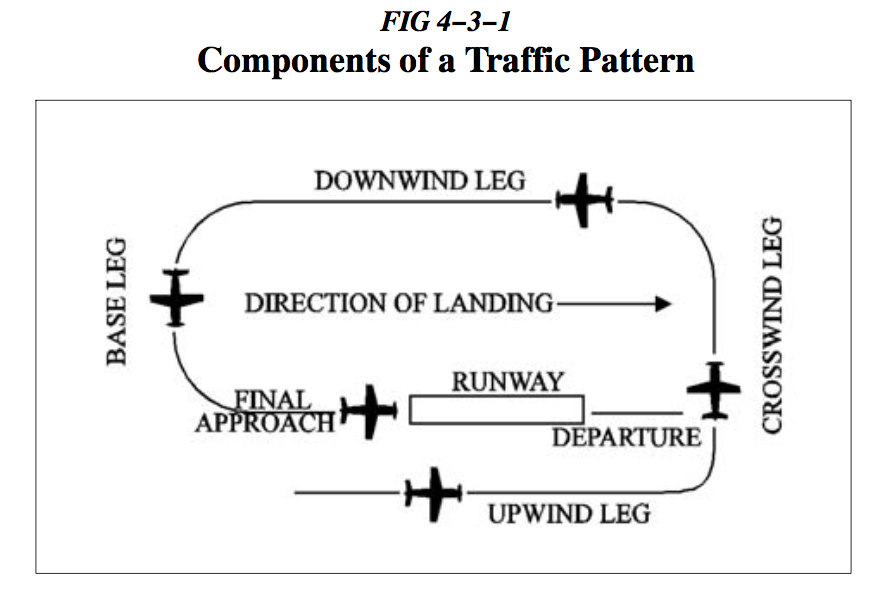
\includegraphics[width=0.7\linewidth]{Figures/Traffic Pattern Legs.png}
			\end{figure}

			In the case of a traffic patten flown at an airport with parallel runways, a no-transgression zone extends between the parallel final and departure legs and should not be entered. Simply track on runway heading until turning crosswind, or after turning final, or until one can depart the traffic pattern.

			\subsubsection{Traffic Pattern at Towered Airports}
				At a towered airport, when not using an instrument approach, or certain visual approaches, a control tower will instruct pilots to join the traffic pattern for a particular runway in a particular direction. For example: ``Join right down wind runway 4R'', or ``Enter left base runway 22L''. Simply enter the traffic pattern as instructed and await landing clearance. To depart the traffic pattern at a towered airport, a pilot should notify tower of their intended direction of departure. Instructions to depart may be issued in reference to a traffic patten leg, radar vectors or visual landmarks.

			\subsubsection{Traffic Pattern at Untowered Airports}
				At an untowered airport, pilots are responsible for remaining alert while in the traffic pattern, and for entering and departing the traffic pattern safely. \\

				The preferred method for entering from the downwind leg side of the pattern is to approach the pattern on a course $45^\circ$ to the downwind leg and join the pattern at midfield. There are several ways to enter the pattern if you are coming from the upwind legs side of the airport. One method of entry from the opposite side of the pattern is to announce your intentions and cross over midfield at least 500 feet above pattern altitude (normally 1,500 feet AGL.) However, if large or turbine aircraft operate at your airport, it is best to remain 2,000 feet AGL so you’re not in conflict with their traffic pattern. When well clear of the pattern - approximately 2 miles - scan carefully for traffic, descend to pattern altitude, then turn right to enter at  $45^\circ$ to the downwind leg at midfield.\footnote{\href[page=135]{./afh.pdf}{AFH - Non-Towered Airports}} \\

				\begin{figure}[H]
					\centering
					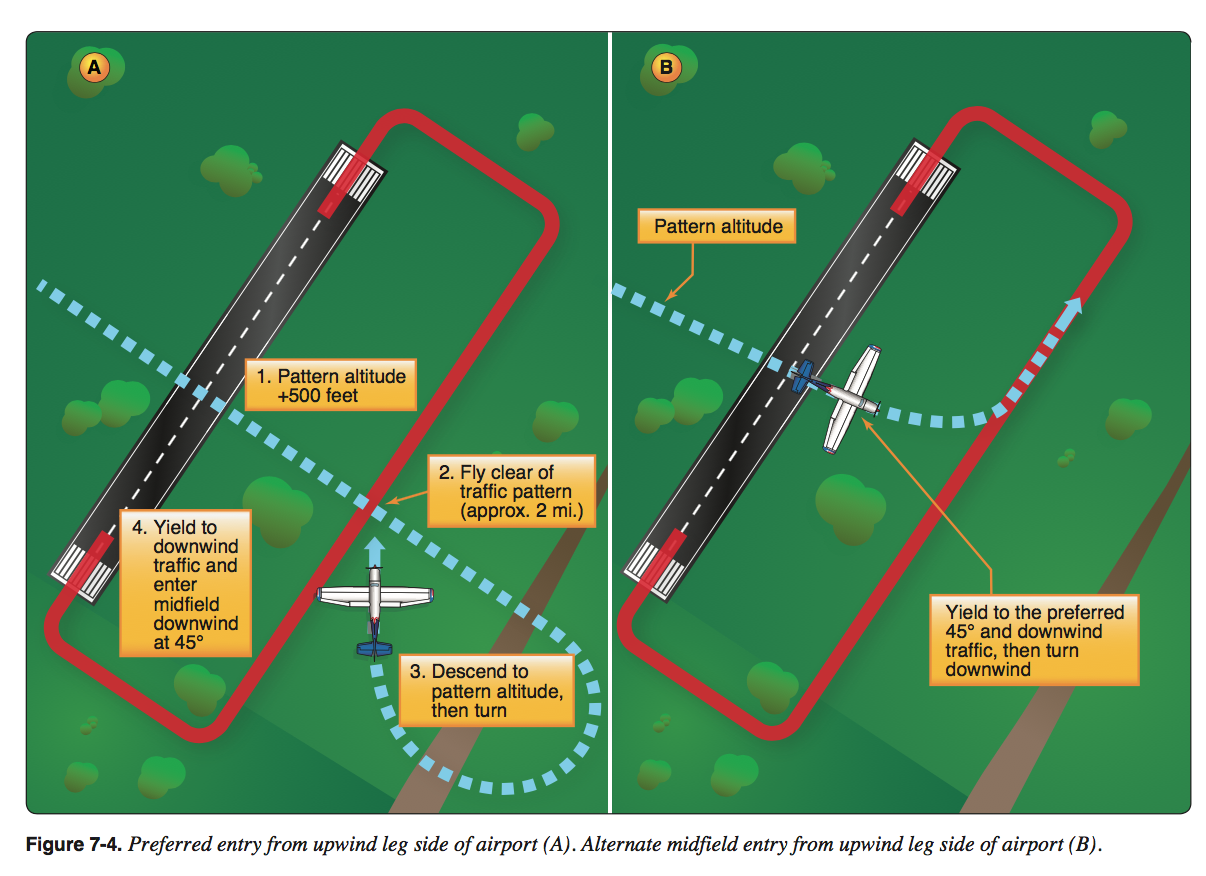
\includegraphics[width=0.7\linewidth]{Figures/Traffic Pattern Entry.png}
				\end{figure}

				While operating at an untowered airport, pilots should monitor and broadcast on the Common Traffic Advisory Frequency (CTAF), MULTICOM (122.9) or other frequency as published. Pilots stating, “Traffic in the area, please advise” is not a recognized Self-Announce Position and/or Intention phrase and should not be used under any condition. \footnote{\href[page=154]{./aim.pdf}{AIM: 4-1-9 Traffic Advisory Practices at Airports Without Operating Control Towers}}\\

				Radio calls should be made as follows:
				\begin{itemize}
					\item \textbf{10 miles distant}: ``[Airport] Traffic [callsign] 10 miles [cardinal direction], inbound [Airport]''
					\item \textbf{5 miles distant}: ``[Airport] Traffic [callsign] 5 miles [cardinal direction], [intentions (overflying, traffic patten entry)] [Airport]''
					\item \textbf{In the traffic pattern} ``[Airport] Traffic [callsign] [left/right] [traffic pattern leg] [runway \#] [Airport]''. While in the downwind one can inform the CTAF what kind of landing/approach one intends to perform.
					\item \textbf{When vacating a runway} ``[Airport] Traffic, [callsign] clear of [runway \#] [optional taxiway] [Airport]''
					\item \textbf{When entering a runway for departure}: ``[Airport] Traffic, [callsign] departing [runway \#] [departure type], [Airport]''
					\item \textbf{Surface Movements}: One should announce runway intentions on the CTAF before taxiing to the runway. One should also always announce when taxiing on a runway or when crossing any runway. However, this shouldn't be done at the expense of preventing airborne aircraft from making their radio calls. 
				\end{itemize}

			\subsubsection{Right of Way}
				Right of Way is of particular importance when operating in a high traffic area such as an airport traffic pattern. Right of way is governed by 14 CFR 91.113\footnote{\href{https://www.law.cornell.edu/cfr/text/14/91.113}{91.113 -  Right-of-way rules: Except water operations}}.

				\begin{enumerate}[label=(\alph*.)]
					\setcounter{enumi}{1}
					\item \textbf{General}. When weather conditions permit, regardless of whether an operation is conducted under instrument flight rules or visual flight rules, vigilance shall be maintained by each person operating an aircraft so as to see and avoid other aircraft. When a rule of this section gives another aircraft the right-of-way, the pilot shall give way to that aircraft and may not pass over, under, or ahead of it unless well clear.
					\item \textbf{In distress.} An aircraft in distress has the right-of-way over all other air traffic.
					\item \textbf{Converging.} When aircraft of the same category are converging at approximately the same altitude (except head-on, or nearly so), the aircraft to the other's right has the right-of-way. If the aircraft are of different categories -
					\begin{enumerate}[label=\arabic*.]
						\item A balloon has the right-of-way over any other category of aircraft;
						\item A glider has the right-of-way over an airship, powered parachute, weight-shift-control aircraft, airplane, or rotorcraft.
						\item  An airship has the right-of-way over a powered parachute, weight-shift-control aircraft, airplane, or rotorcraft.\\	
						However, an aircraft towing or refueling other aircraft has the right-of-way over all other engine-driven aircraft.
					\end{enumerate}

					\item \textbf{Approaching head-on.} When aircraft are approaching each other head-on, or nearly so, each pilot of each aircraft shall alter course to the right.

					\item \textbf{Overtaking.} Each aircraft that is being overtaken has the right-of-way and each pilot of an overtaking aircraft shall alter course to the right to pass well clear.

					\item \textbf{Landing.} Aircraft, while on final approach to land or while landing, have the right-of-way over other aircraft in flight or operating on the surface, except that they shall not take advantage of this rule to force an aircraft off the runway surface which has already landed and is attempting to make way for an aircraft on final approach. When two or more aircraft are approaching an airport for the purpose of landing, the aircraft at the lower altitude has the right-of-way, but it shall not take advantage of this rule to cut in front of another which is on final approach to land or to overtake that aircraft.
				\end{enumerate}
%done
\newpage
\section{Cross Country Planning, In-Flight procedures, \& Navigation}
	\subsection{Aeronautical Chart Usage}
		There are a variety of aeronautical charts available for use by pilots. VFR pilots use charts at two different scales: sectional charts (1:500000) and Terminal Area Charts (TACs) (1:250000). Both depict information similarly, although a TAC displays information pertinant to busy airspaces in greater detail than an overlying sectional chart. On the reverse of a TAC, one can often find information about VFR flyway routes to navigate around the central Class B airport.\\ 

		On a sectional chart:
			\begin{itemize}
				\item Lines of latitude and longitude are marked 30' apart
				\item VOR compass roses have a radius of 20nmi
				\item Victor airways have distances between legs boxed in blue. 
			\end{itemize}

		\begin{figure}
			\centering
			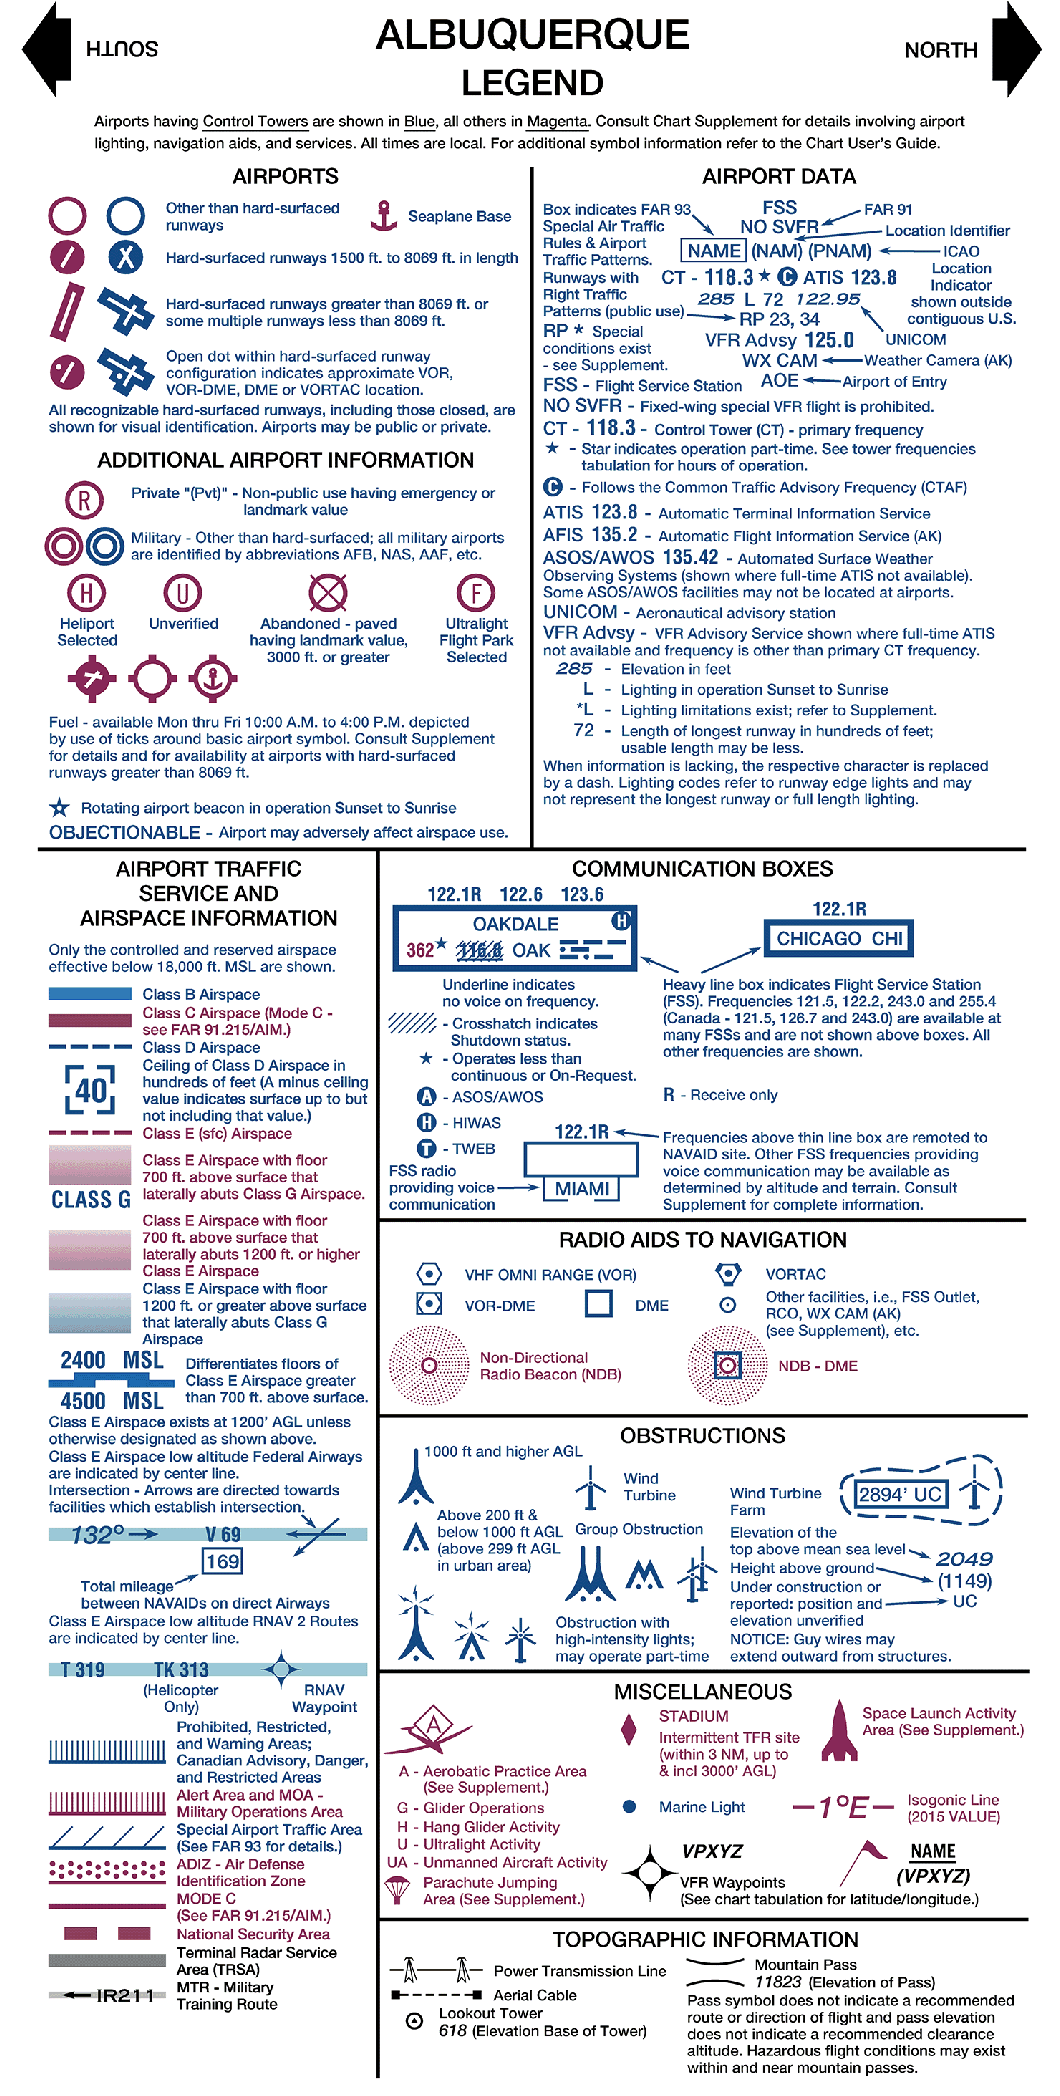
\includegraphics[width=0.7\linewidth]{Figures/Sectional Legend.png}
			\caption{Sectionals and TACs use the legend above.}
		\end{figure}

		\subsubsection{Chart Supplement}
			The Chart Supplement, as the name implies, acts as a companion to the information depicted on a sectional or terminal area chart. It contains more detailed information about Airports, NAVAIDs, FSS, and about the geographic region than can be illustrated on a chart. Of particular importance to cross-country planning in the Chart Suppliment is information about runway lengths, traffic pattern direction and fuel availability.
	\subsection{Victor Airways}
	\subsection{Radio Aids to Navigation: VOR \& NDB}
		\subsubsection{VOR: Very High Frequency (VHF) Omnidirectional Range}
			The VOR system is present in three slightly different navigation aids (NAVAIDs): VOR, VOR/distance measuring equipment (DME)(discussed in a later section), and VORTAC. By itself it is known as a VOR, and it provides magnetic bearing information to and from the station. When a DME is also installed with a VOR, the NAVAID is referred to as a VOR/DME. When military tactical air navigation (TACAN) equipment is installed with a VOR, the NAVAID is known as a VORTAC. DME is always an integral part of a VORTAC.\\

			The course or radials projected from the station are referenced to magnetic north at the time of VOR installation. A \textbf{radial} is defined as a line extending outward from the VOR station. A \textbf{bearing}, is the line extending to a VOR station. The magnetic variation that the VOR is referenced by is listed in the chart supplement.\\

			VORs and VORTACs are classed according to operational use. There are three classes:
			\begin{enumerate}
				\item T(Terminal)
					\begin{itemize} \item 12,000' and below: 25 miles range \end{itemize}
				\item L(Low altitude):
					\begin{itemize} \item Below 18,000': 40 miles range \end{itemize}
				\item H(High altitude): 
					\begin{itemize}
						\item Below 14,500': 40 miles range
						\item Within the conterminous 48 states only, between 14,500' and 17,999': 100 miles range
						\item 18,000' - FL 450: 130 miles range
						\item FL 450 - 60,000': 100 miles range
					\end{itemize}
			\end{enumerate}

			The VOR transmitting station can be positively identified by its Morse code identification or by a recorded voice identification that states the name of the station followed by ``VOR.'' Many FSSs transmit voice messages on the same frequency that the VOR operates. Voice transmissions should not be relied upon to identify stations because many FSSs remotely transmit over several omniranges that have names different from that of the transmitting FSS. If the VOR is out of service for maintenance, the coded identification is removed and not transmitted. This serves to alert pilots that this station should not be used for navigation.\footnote{\href[page=410]{./phak.pdf}{PHAK: Navigation - Very High Frequency (VHF) Omnidirectional Range (VOR)}}

			\paragraph{VOR Usage}
				A VOR, without DME cannot be used on its own to locate oneself. Instead two VORs must be used. The interesection two radials recieved at a particular point gives a position. When equipped with DME, all that is needed to define a position is a radial and distance. ($r,\theta$) Note that a DME gives slant range, not distance along the ground. This makes DME measurements less accurate at shorter distances.\\

				A VOR can also be used to navigate to an arbitrary point. Without DME, one can locate the intercepting radials of a given point, then intercept one radial, and fly along that radial until the second radial is intercepted. (or bearing, if using a bearing pointer)

		\subsubsection{NDB: Non-directional Beacon}
			Unlike a VOR, an NDB does not transmit any inherent direction information (hence ``non-direction''). An Automatic Direction Finder (ADF) is the instrument used to use an NDB. The ADF aircraft equipment consists of a tuner, which is used to set the desired station frequency, and the navigational display. The ADF simply points in the direction of the tuned NDB. In principle the ADF can be tuned to any AM radio station, and if the location of an AM antenna is known, this can be used for navigation. One of the disadvantages that should be considered when using low frequency (LF) for navigation is that LF signals are very susceptible to electrical disturbances, such as lightning. These disturbances create excessive static, needle deviations, and signal fades. An ADF also transmits an identifier in morse code.\footnote{\href[page=417]{./phak.pdf}{PHAK: Navigation - Automatic Direction Finder (ADF)}}
	\subsection{GPS (Global Positioning System) Usage}
		The GPS is a satellite-based radio navigation system. A minimum of four satellites is necessary to establish an accurate three-dimensional position. Visual GPS waypoints consist of five letters, beginning with the letters ``VP''. In addition, other VFR \& IFR way-points can be used in a GPS system, along with any airport or radio navigational aid located in the GPS database. One can also input arbitrary points using their latitude and longitude. \footnote{\href[page=418]{./phak.pdf}{PHAK: Navigation - Global Positioning System}}

	\subsection{Pilotage, Dead Reckoning, \& Route Planning}
		\subsubsection{Pilotage} is navigation by reference to landmarks or checkpoints. It is a method of navigation that can be used on any course that has adequate checkpoints, but it is more commonly used in conjunction with dead reckoning and VFR radio navigation. The checkpoints selected should be prominent features visible from the area of the flight.\footnote{\href[page=400]{./phak.pdf}{PHAK: Navigation - Pilotage}}

		\subsubsection{Dead reckoning} is navigation solely by means of computations based on time, airspeed, distance, and direction. The products derived from these variables, when adjusted by wind speed and velocity, are heading and GS. The predicted heading takes the aircraft along the intended path and the GS establishes the time to arrive at each checkpoint and the destination. Except for flights over water, dead reckoning is usually used with pilotage for cross-country flying. The heading and GS, as calculated, is constantly monitored and corrected by pilotage as observed from checkpoints.\footnote{\href[page=401]{./phak.pdf}{PHAK: Navigation - Dead Reckoning}}

		\subsubsection{Magnetic Variation, Magnetic Course, Headings, Wind Correction Angles}
			\begin{itemize}
				\item True Course: direction of the line connecting two desired • points, drawn on the chart and measured clockwise
				\item Variation: obtained from the isogonic line on the chart (added to TH if west; subtracted if east)
				\item Magnetic Heading: an intermediate step in the conversion (obtained by applying variation to TH) in degrees from true north on the mid-meridian
				\item Wind Correction Angle: determined from the wind triangle. (Added to TC if the wind is from the right; subtracted if wind is from the left)
				\item True Heading: direction measured in degrees clockwise from true north, in which the nose of the plane should point to remain on the desired course
				\item Deviation: obtained from the deviation card on the aircraft (added to or subtracted from MH, as indicated). Deviation is caused by magnetic fields induced by current within the airplane.
				\item Compass heading : reading on the compass (found by applying deviation to MH) that is followed to remain on the desired course.
			\end{itemize}
		\subsubsection{Flight Planning}
			Title 14 of the Code of Federal Regulations (14 CFR) part 91 states, in part, that before beginning a flight, the pilot in command (PIC) of an aircraft shall become familiar with all available information concerning that flight. For flights not in the vicinity of an airport, this must include information on available current weather reports and forecasts, fuel requirements, alternatives available if the planned flight cannot be completed, and any known traffic delays of which the PIC has been advised by ATC.\\

			Determine the takeoff and landing distances from the appropriate charts, based on the calculated load, elevation of the airport, and temperature; then compare these distances with the amount of runway available. Remember, the heavier the load and the higher the elevation, temperature, or humidity, the longer the takeoff roll and landing roll and the lower the rate of climb.\\

			Check the fuel consumption charts to determine the rate of fuel consumption at the estimated flight altitude and power settings. Calculate the rate of fuel consumption, and compare it with the estimated time for the flight so that refueling points along the route can be included in the plan.

			Appropriate checkpoints should be selected along the route and noted in some way. These should be easy-to-locate points, such as large towns, large lakes and rivers, or combinations of recognizable points, such as towns with an airport, towns with a network of highways, and railroads entering and departing. Victor airways are ``easy'' ways to plan a cross country but note that victor airways connect between VORs, without much regard taken to environmental hazards or suitable diversion locations. 

			The course and areas on either side of the planned route should be checked to determine if there is any type of airspace with which the pilot should be concerned or which has special operational requirements.\footnote{\href[page=401]{./phak.pdf}{PHAK: Navigation - Flight Planning}}

			VFR cruising altitudes above 3000 AGL but below 18000 MSL:\footnote{\href[page=128]{./aim.pdf}{AIM: 3-1-5 VFR Cruising Altitudes and Flight Levels}}
			\begin{itemize}
				\item Ground track $0^\circ - 179^\circ$: Odd thousands + 500 feet (3500, 5500, ...)
				\item Ground track $180^\circ - 259^\circ$: Even thousands + 500 feet (4500, 6500, ...)
			\end{itemize}

			\paragraph{Navigation Log}

			A navigation log lists a flight's visual waypoints, any relavant navigation aids, planned altitude, leg distance and true course. The following information should be calculated using temperatures and winds aloft: Wind Correction Angles, True Heading, Magnetic Variation, Magnetic Heading, Compass Deviation, Compass Heading, Ground Speed, Time Enroute, and Fuel Burn. Estimated fuel burn should be calculated using published cruise performance data in the aircraft's POH/AFM.
	\subsection{VFR Flight Plan}
		Filing a flight plan is not required by regulations; however, it is a good operating practice since the information contained in the flight plan can be used in search and rescue in the event of an emergency. Flight plans can be filed in the air by radio, but it is best to file a flight plan by phone just before departing. After takeoff, contact the FSS by radio and give them the takeoff time so the flight plan can be activated. When a VFR flight plan is filed, it is held by the FSS until 1 hour after the proposed departure time and then canceled unless: the actual departure time is received; a revised proposed departure time is received; or at the time of filing, the FSS is informed that the proposed departure time is met, but actual time cannot be given because of inadequate communication. \footnote{\href[page=401]{./phak.pdf}{PHAK: Navigation - Filing a VFR Flight Plan}}
	\subsection{In-Flight Weather Information}
		One can recieve up-to-date weather information from several sources:
			\begin{itemize}
				\item FSS: a flight service station can provide over radio current weather information and advisories
				\item HIWAS: Hazardous Inflight Weather Advisory Service (HIWAS), available in the 48 conterminous states, is an automated continuous broadcast of hazardous weather information over selected VOR navigational aids.he broadcasts include advisories such as AIRMETS, SIGMETS, convective SIGMETS, and urgent PIREPs.  
				\item ATIS/AWOS/ASOS: any of these, if available will provide the current weather at an airport. This is helpful, when flying in the vicinity of an airport enroute.
				\item ADS-B weather: ADS-B offers weather radar data, and updated SIGMETs, AIRMETs, NOTAMs, TFRs, METARs, and TAFs.
			\end{itemize}
	\subsection{Diversions}
		A diversion may be necessary due to unpredicted weather conditions, a system malfunction, or poor preflight planning. Before any cross-country flight, check the charts for airports or suitable landing areas along or near the route of flight. After selecting the most appropriate alternate destination, approximate the magnetic course to the alternate using a compass rose or airway on the sectional chart. If time permits, try to start the diversion over a prominent ground feature. However, in an emergency, divert promptly toward your alternate destination. Attempting to complete all plotting, measuring, and computations involved before diverting to the alternate destination may only aggravate an actual emergency. Once established on course, note the time, and then use the winds aloft nearest to your diversion point to calculate a heading and GS. Once a GS has been calculated, determine a new arrival time and fuel consumption.\footnote{\href[page=422]{./phak.pdf}{PHAK: Navigation - Flight Diversion}}
	\subsection{Lost Procedures}
	One can get lost for any number of reasons: a momentary lapse of attention, accidental flight into IMC or disorientation. The following steps are generic to any ``lost'' situation.
	4 Cs:
	\begin{itemize}
		\item \textbf{C}limb - the higher altitude allows better communication and visual range to find landmarks
		\item \textbf{C}ommunicate - communicate over the relavant ATC frequency to get help. 121.5 is also an option if one is not in communication
		\item \textbf{C}onfess - once communication is established, ask for help
		\item \textbf{C}omply - follow instructiions. This will likely include a squawk code and radar vectors.
	\end{itemize}
%done
\newpage
\section{ATC \& Airspaces}
	\subsection{Classes of Airspace}
		Airspace is a generic term that covers the different classifications of airspace and defined dimensions.
		\begin{figure}[H]
			\centering
			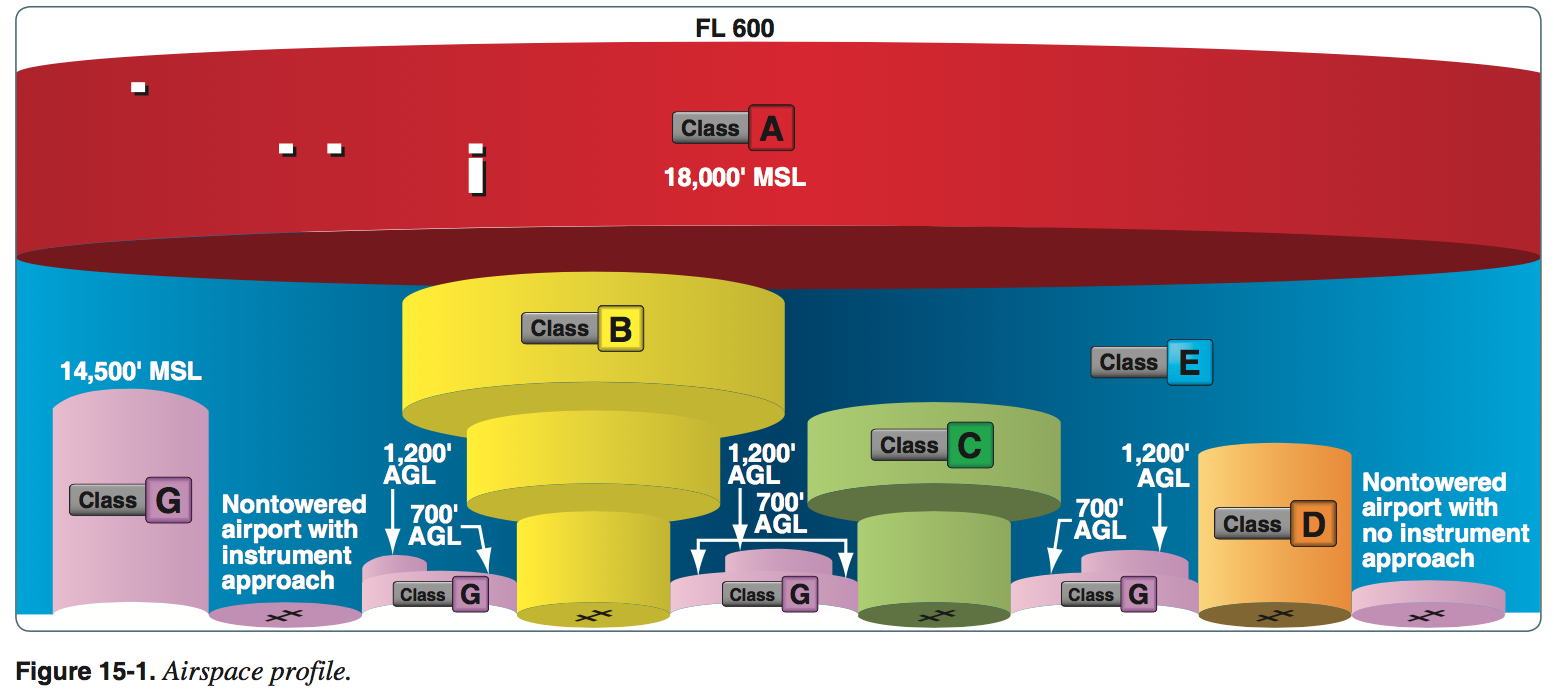
\includegraphics[width=\linewidth]{Figures/Airspace.png}
		\end{figure}
		\subsubsection{Class A}\footnote{\href[page=130]{./aim.pdf}{AIM: 3-2-2 Class A Airspace}}
			\begin{itemize}
				\item located at altitudes [FL180, FL600] MSL over the 48 contiguous states and Alaska
				\item all operations are IFR
				\item no weather minimums
				\item not marked on a sectional
				\item Pilot must be Instrument rated, plane must be IFR equipped
			\end{itemize}
		\subsubsection{Class B}\footnote{\href[page=130]{./aim.pdf}{AIM: 3-2-3 Class B Airspace}}
			\begin{itemize}
				\item located around the busiest airports
				\item General Dimensions: an upside down wedding cake up to 10000 MSL, tailored to operational requirements.
				\item IFR \& VFR traffic
				\item 3 sm visbility, clear of clouds
				\item Speed limit: 250kts within B, 200kts beneath class B airspace
				\item Clearance must be recieved prior to entry (IFR clearance implictly acts as a Bravo clearance)
				\item All aircraft recieve sequencing and separation from other aircraft while operating within Class B airspace.
				\item Marked on sectional as solid blue lines; with floor and celing MSL altitudes labeled in blue
				\item For IFR operations: VOR reciever or RNAV system
				\item For all operations: Mode C transponder or better (30sm radius from primary airport) and within class B
			\end{itemize}
		\subsubsection{Class C}\footnote{\href[page=132]{./aim.pdf}{AIM: 3-2-4 Class C Airspace}}
			\begin{itemize}
				\item located around moderately busy airports with a control tower and radar approach control
				\item General dimensions: inner region extends from [Surface, 4000 AGL] at a radius of 5 nmi, outer region from [1200 AGL, 4000 AGL] to a radius of 10 nmi.
				\item IFR \& VFR traffic
				\item 3 sm visbility, 500 below, 1000 above, 2000 feet from clouds
				\item Speed limit: 200kts at or below 2,500 feet above the surface within 4 nautical miles of the primary airport of a Class C.
				\item Contact with approach control must be made prior to entry; ideally 20 nmi distant from the central airport, and communications must be maintained
				\item Traffic separation is provided within the Class C airspace and the outer area after two-way radio communications and radar contact are established. 
				\item No certification requirement
				\item Marked on a sectional with a solid magenta line; floor and ceiling MSL altitudes labeled in magenta
				\item For all operations: a two-way radio, and a mode C transponder or better is required.
			\end{itemize}
		\subsubsection{Class D}\footnote{\href[page=136]{./aim.pdf}{AIM: 3-2-5 Class D Airspace}}
			\begin{itemize}
				\item located around less busy airports that still have control towers
				\item General dimensions: single cylinder shaped region extending up to 2500 AGL to a custom radius tailored to the needs of the airport
				\item Where a Class D surface area is part-time, the airspace may revert to either a Class E surface area or Class G airspace. 
				\item IFR \& VFR traffic
				\item 3 sm visbility, 500 below, 1000 above, 2000 feet from clouds
				\item Speed Limit: 200kts unless otherwise authorized or required by ATC, no person may operate an aircraft at or below 2,500 feet above the surface within 4 nautical miles of the primary airport of a Class D.
				\item Communication with airport control tower must be established prior to entry; if taking off from a satellite airport communication must established as soon as practical
				\item Traffic service is limited, no separation services are automatically provided to VFR aircraft.
				\item No certification requirement
				\item Marked on a sectional with a dashed blue line; ceiling altitude is boxed in AGL. When preceded with a -, this altitude is exclusive.
				\item For all operations: a two-way radio is required
			\end{itemize}
		\subsubsection{Class E}\footnote{\href[page=137]{./aim.pdf}{AIM: 3-2-6 Class E Airspace}}
			\begin{itemize}
				\item the bulk of airspace below 18000 MSL (many non-towered airports, to protect instrument procedures at Class C/D, victor airways).
				\item IFR \& VFR traffic
				\item 3 sm visbility, 500 below, 1000 above, 2000 feet from clouds below 10000 MSL
				\item 5 sm visbility, 1000 below, 1000 above, 1 sm from clouds above 10000 MSL
				\item 250 kts speed limit below 10000 MSL, Mach 1.0 above
				\item Sectional and other charts depict all locations of Class E airspace with bases below 14,500 feet MSL. In areas where charts do not depict a class E base, class E begins at 14,500 feet MSL.
				\item  In most areas, the Class E airspace base is 1,200 feet AGL. In many other areas, the Class E airspace base is either the surface or 700 feet AGL. Some Class E airspace begins at an MSL altitude depicted on the charts, instead of an AGL altitude.
				\item Class E airspace typically extends up to, but not including, 18,000 feet MSL (the lower limit of Class A airspace). All airspace above FL 600 is Class E airspace.
				\item No certification requirement
				\item No equipment requirement.
				\item No separation services are provided to VFR aircraft.
				\item Extends from 700 AGL in areas surrounded by a magenta vignette, from 1200 AGL in areas surrounded by a blue vignette, from altitudes labeled on altenating blue lines, extends above FL 600.
				\item Extends from surface in areas enclosed by a dashed magenta line. (usually to protect instrument procedures)
			\end{itemize}
		\subsubsection{Class G}\footnote{\href[page=139]{./aim.pdf}{AIM: Section 3 - Class G Airspace}}
			\begin{itemize}
				\item Located wherever Classes A-E have not been designated
				\item Uncontrolled traffic
				\item IFR traffic must remain at least 1,000 feet (2,000 feet in designated mountainous terrain) above the highest obstacle within a horizontal distance of 4 nautical miles from the course to be flown.
				\item Class G extends from the surface to the floor of the Class E above
				\item VFR Day visbility requirements (below 1200 AGL): 1 sm visibility, clear of clouds
				\item VFR Day visbility requirements (above 1200 AGL and below 10000 MSL): 1 sm visibility, 500 feet below, 1000 feet above, 2000 feet from clouds
				\item VFR Night visbility requirements (surface to 10000 MSL): 3 sm visibility, 500 feet below, 1000 feet above, 2000 feet from clouds
				\item VFR Visibility requirements above 1200 AGL and 10000 MSL: 5 sm visibility, 1000 feet below, 1000 feet above, 1 sm from clouds.
				\item No certification requirement.
				\item No equipment requirement.
				\item Its boundaries are defined by the boundaries of class E.
			\end{itemize}
	\subsection{Special Use Airspace}
		\begin{enumerate}
			\item \textbf{Prohibited areas:} Prohibited areas contain airspace of defined dimensions within which the flight of aircraft is prohibited. Such areas are established for security or other reasons associated with the national welfare. These areas are published in the Federal Register and are depicted on aeronautical charts. The area is charted as a “P” followed by a number (e.g., P-40).\footnote{\href[page=141]{./aim.pdf}{AIM: 3-4-2 Prohibited Areas}}
			\item \textbf{Restricted areas:} Restricted areas are areas where operations are hazardous to nonparticipating aircraft and contain airspace within which the flight of aircraft, while not wholly prohibited, is subject to restrictions. Activities within these areas must be confined because of their nature, or limitations may be imposed upon aircraft operations that are not a part of those activities, or both. Restricted areas denote the existence of unusual, often invisible, hazards to aircraft (e.g., artillery firing, aerial gunnery, or guided missiles). IFR flights may be authorized to transit the airspace and are routed accordingly. Penetration of restricted areas without authorization from the using or controlling agency may be extremely hazardous to the aircraft and its occupants. \footnote{\href[page=141]{./aim.pdf}{AIM: 3-4-3 Restricted Areas}}
			\item \textbf{Warning areas:} Warning areas are similar in nature to restricted areas; however, the United States government does not have sole jurisdiction over the airspace. A warning area is airspace of defined dimensions, extending from 3 NM outward from the coast of the United States, containing activity that may be hazardous to nonparticipating aircraft. The purpose of such areas is to warn nonparticipating pilots of the potential danger. A warning area may be located over domestic or international waters or both. The airspace is designated with a “W” followed by a number (e.g., W-237). \footnote{\href[page=141]{./aim.pdf}{AIM: 3-4-4 Warning Areas}}
			\item \textbf{Military operation areas (MOAs):} MOAs consist of airspace with defined vertical and lateral limits established for the purpose of separating certain military training activities from IFR traffic. Whenever an MOA is being used, nonparticipating IFR traffic may be cleared through an MOA if IFR separation can be provided by ATC. Otherwise, ATC reroutes or restricts nonparticipating IFR traffic. MOAs are depicted on sectional, VFR terminal area, and en route low altitude charts and are not numbered (e.g., “Camden Ridge MOA”). \footnote{\href[page=142]{./aim.pdf}{AIM: 3-4-5 Millitary Operations Areas}}
			\item \textbf{Alert areas:} Alert areas are depicted on aeronautical charts with an “A” followed by a number (e.g., A-211) to inform nonparticipating pilots of areas that may contain a high volume of pilot training or an unusual type of aerial activity. Pilots should exercise caution in alert areas. All activity within an alert area shall be conducted in accordance with regulations, without waiver, and pilots of participating aircraft, as well as pilots transiting the area, shall be equally responsible for collision avoidance.\footnote{\href[page=142]{./aim.pdf}{AIM: 3-4-6 Alert Areas}}
			\item \textbf{Controlled firing areas:} CFAs contain activities that, if not conducted in a controlled environment, could be hazardous to nonparticipating aircraft. The difference between CFAs and other special use airspace is that activities must be suspended when a spotter aircraft, radar, or ground lookout position indicates an aircraft might be approaching the area. There is no need to chart CFAs since they do not cause a nonparticipating aircraft to change its flight path. \footnote{\href[page=142]{./aim.pdf}{AIM: 3-4-7 Controlled Firing Areas}}
			\item \textbf{National Security Areas:} National Security Areas consist of airspace of defined vertical and lateral dimensions established at locations where there is a requirement for increased security and safety of ground facilities. Pilots are requested to voluntarily avoid flying through the depicted NSA.\footnote{\href[page=142]{./aim.pdf}{AIM: 3-4-8 National Security Areas}}
		\end{enumerate}
	\subsection{Other Airspace Areas}
		\begin{enumerate}
			\item \textbf{Military Training Routes}:
				Established below 10,000 feet MSL for operations at speeds in excess of 250 knots.\footnote{\href[page=143]{./aim.pdf}{AIM: 3-5-2 Millitary Training Routes}}
				\begin{itemize}
					\item IFR Military Training Route are labelled with IR
					\item VFR Military Training Routes are labelled with VR
					\item MTRs with no segment above 1,500 feet AGL must be identified by four number characters; e.g., IR1206, VR1207.
					\item MTRs that include one or more segments above 1,500 feet AGL must be identified by three number characters; e.g., IR206, VR207.
					\item Charted on sectional and Low IFR Enroute charts
				\end{itemize}
			\item \textbf{Temporary Flight Restrictions (TFRs)}\footnote{\href[page=144]{./aim.pdf}{AIM: 3-5-3 Temporary Flight Restrictions}}:
				\begin{itemize}
					\item Protect persons and property in the air or on the surface from an existing or imminent hazard associated with an incident on the surface when the presence of low flying aircraft would magnify, alter, spread, or compound that hazard
					\item Provide a safe environment for the operation of disaster relief aircraft
					\item Prevent an unsafe congestion of sightseeing aircraft above an incident or event which may generate a high degree of public interest
					\item Protect declared national disasters for humanitarian reasons in the State of Hawaii 
					\item Protect the President, Vice President, or other public figures
					\item Provide a safe environment for space agency operations 
					\item The facility establishing a temporary flight restrictions area will format a NOTAM beginning with the phrase “FLIGHT RESTRICTIONS” followed by: the location of the temporary flight restrictions area; the effective period; the area defined in statute miles; the altitudes affected; the FAA coordination facility and commercial telephone number
				\end{itemize}
			\item \textbf{Parachute Jump Aircraft Operations}\footnote{\href[page=147]{./aim.pdf}{AIM: 3-5-4 Parachute Jump Aircraft Operations}}: These areas are labelled with a parachute on a sectional chart. Contact the local center/approach control for information, or monitor the local CTAF.
			\item \textbf{Published VFR Routes}\footnote{\href[page=147]{./aim.pdf}{AIM: 3-5-5 Published VFR Routes}}: Published VFR routes exist for transitioning around, under and through complex airspace such as Class B airspace.
				\begin{itemize}
					\item VFR Flyways: A VFR Flyway is defined as a general flight path not defined as a specific course, for use by pilots in planning flights into, out of, through or near complex terminal airspace to avoid Class B airspace. An ATC clearance is NOT required to fly these routes. Pilot adherence to VFR rules must be exercised at all times. Further, when operating beneath Class B airspace, communications must be established and maintained between your aircraft and any control tower while transiting the Class B, Class C, and Class D surface areas of those airports under Class B airspace.
					\item VFR Corridors: A VFR corridor is defined as airspace through Class B airspace, with defined vertical and lateral boundaries, in which aircraft may operate without an ATC clearance or communication with air traffic control. These corridors are, in effect, a “hole” through Class B airspace. 
					\item Class B Airspace VFR Transition Routes: A Class B Airspace VFR Transition Route is defined as a specific flight course depicted on a TAC for transiting a specific Class B airspace. These routes include specific ATC-assigned altitudes, and pilots must obtain an ATC clearance prior to entering Class B airspace on the route. On initial contact, pilots should advise ATC of their position, altitude, route name desired, and direction of flight. After a clearance is received, pilots must fly the route as depicted and, most importantly, adhere to ATC instructions.
				\end{itemize}
			\item \textbf{Terminal Radar Service Areas(TRSA)}\footnote{\href[page=151]{./aim.pdf}{AIM: 3-5-6 Terminal Radar Service Area (TRSA)}}\footnote{\href[page=383]{./phak.pdf}{Airspace - Terminal Radar Service Areas (TRSAs)}}: TRSAs exist around certain high traffic areas. Pilots operating under VFR are encouraged to contact the radar approach control and avail themselves of the TRSA Services. TRSAs are areas where participating pilots can receive additional radar services. The purpose of the service is to provide separation between all IFR operations and participating VFR aircraft. TRSAs are depicted on VFR sectional and terminal area charts with a solid black line and altitudes for each segment. The Class D portion is charted with a blue segmented line.
			\item \textbf{Special Air Traffic Rules (SATR) and Special Flight Rules Area (SFRA)}\footnote{\href[page=151]{./aim.pdf}{AIM: 3-5-7 Special Air Traffic Rules (SATR) and Special Flight Rules Area (SFRA)}}: The Code of Federal Regulations (CFR) prescribes special air traffic rules for aircraft operating within the boundaries of certain designated airspace.  Each person operating an aircraft to, from, or within airspace designated as a SATR area or SFRA must adhere to the special air traffic rules set forth in 14 CFR Part 93, as applicable, unless otherwise authorized or required by ATC. SFRAs are depicted on VFR sectional, terminal area, and helicopter route charts.
		\end{enumerate}
	\subsection{ATC Services}
		The primary purpose of the ATC system is to prevent a collision between aircraft operating in the system and to organize and expedite the flow of traffic. In addition to its primary function, the ATC system has the capability to provide (with certain limitations) additional services. The ability to provide additional services is limited by many factors, such as the volume of traffic, frequency congestion, quality of radar, controller workload, higher priority duties, and the pure physical inability to scan and detect those situations that fall in this category. It is recognized that these services cannot be provided in cases in which the provision of services is precluded by the above factors.\footnote{\href[page=383]{./phak.pdf}{PHAK: Airspace - Air Traffic Control and the National Airspace System}}
		\subsubsection{ATC Clearances}
			A clearance issued by ATC is predicated on known traffic and known physical airport conditions. An ATC clearance means an authorization by ATC, for the purpose of preventing collision between known aircraft, for an aircraft to proceed under specified conditions within controlled airspace. IT IS NOT AUTHORIZATION FOR A PILOT TO DEVIATE FROM ANY RULE, REGULATION, OR MINIMUM ALTITUDE NOR TO CONDUCT UNSAFE OPERATION OF THE AIRCRAFT.\\

			If ATC issues a clearance that would cause a pilot to deviate from a rule or regulation, or in the pilot’s opinion, would place the aircraft in jeopardy, IT IS THE PILOT’S RESPONSIBILITY TO REQUEST AN AMENDED CLEARANCE. Similarly, if a pilot prefers to follow a different course of action, such as make a 360 degree turn for spacing to follow traffic when established in a landing or approach sequence, land on a different runway, takeoff from a different intersection, takeoff from the threshold instead of an intersection, or delay operation, THE PILOT IS EXPECTED TO INFORM ATC ACCORDINGLY. When the pilot requests a different course of action, however, the pilot is expected to cooperate so as to preclude disruption of traffic flow or creation of conflicting patterns. The pilot is also expected to use the appropriate aircraft call sign to acknowledge all ATC clearances, frequency changes, or advisory information.\footnote{\href[page=213]{./aim.pdf}{AIM: 4-4-1 Clearance}}\\

			\paragraph{Amended Clearances}\footnote{\href[page=214]{./aim.pdf}{AIM: 4-4-4 Amended Clearances}} Amendments to the initial clearance will be issued at any time an air traffic controller deems such action necessary to avoid possible confliction between aircraft. Clearances will require that a flight ``hold'' or change altitude prior to reaching the point where standard separation from other IFR traffic would no longer exist. Pilots have the privilege of requesting a different clearance from that which has been issued by ATC if they feel that they have information which would make another course of action more practicable or if aircraft equipment limitations or company procedures forbid compliance with the clearance issued.

		\subsubsection{Special VFR Clearances}
			An ATC clearance must be obtained prior to operating within a Class B, Class C, Class D, or Class E surface area when the weather is less than that required for VFR flight. A VFR pilot may request and be given a clearance to enter, leave, or operate within most Class D and Class E surface areas and some Class B and Class C surface areas in special VFR conditions, traffic permitting, and providing such flight will not delay IFR operations. All special VFR flights must remain clear of clouds. The visibility requirements for special VFR aircraft (other than helicopters) are:\footnote{\href[page=215]{./aim.pdf}{AIM: 4-4-6 Special VFR Clearances}}
				\begin{enumerate}
					\item At least 1 statute mile flight visibility for operations within Class B, Class C, Class D, and Class E surface areas.
					\item At least 1 statute mile ground visibility if taking off or landing. If ground visibility is not reported at that airport, the flight visibility must be at least 1 statute mile.
				\end{enumerate}
			When a control tower is located within the Class B, Class C, or Class D surface area, requests for clearances should be to the tower. In a Class E surface area, a clearance may be obtained from the nearest tower, FSS, or center.\\
			Special VFR clearances are effective within Class B, Class C, Class D, and Class E surface areas only. ATC does not provide separation after an aircraft leaves the Class B, Class C, Class D, or Class E surface area on a special VFR clearance.
		\subsubsection{Traffic Separation \& Surveillance}
			Visual separation is a means employed by ATC to separate aircraft in terminal areas and en route airspace in the NAS. There are two methods employed to effect this separation: the tower controller sees the aircraft involved and issues instructions, as necessary, to ensure that the aircraft avoid each other or the pilot sees the other aircraft involved and upon instructions from the controller provides separation by maneuvering the aircraft to avoid it. A pilot’s acceptance of instructions to follow another aircraft or provide visual separation from it is an acknowledgment that the pilot will maneuver the aircraft as necessary to avoid the other aircraft or to maintain in−trail separation and is also an acknowledgment that the pilot accepts the responsibility for wake turbulence separation. Visual separation is prohibited behind super aircraft.\\

			 Since the eye can focus only on a narrow viewing area, effective scanning is accomplished with a series of short, regularly spaced eye movements that bring successive areas of the sky into the central visual field. Each movement should not exceed ten degrees, and each area should be observed for at least one second to enable collision detection.\footnote{\href[page=222]{./aim.pdf}{AIM: 4-4-14 Visual Separation}}\\

			 \textbf{Use of Visual Clearing Procedures}\footnote{\href[page=223]{./aim.pdf}{AIM: 4-4-15 Use of Visual Clearing Procedures}}:
			 	\begin{enumerate}
			 		\item \textbf{Before Takeoff}: Prior to taxiing onto a runway or landing area in preparation for takeoff, pilots should scan the approach areas for possible landing traffic.
			 		\item \textbf{Climbs and Descents}: During climbs and descents in flight conditions which permit visual detection of other traffic, pilots should execute gentle banks, left and right at a frequency which permits continuous visual scanning of the airspace about them.
			 		\item \textbf{Straight and Level}: Sustained periods of straight and level flight in conditions which permit visual detection of other traffic should be broken at intervals with appropriate clearing procedures to provide effective visual scanning.
			 		\item \textbf{Traffic Pattern}: Entries into traffic patterns while descending create specific collision hazards and should be avoided.
			 		\item \textbf{Traffic at VOR Sites}: All operators should emphasize the need for sustained vigilance in the vicinity of VORs and airway intersections due to the convergence of traffic.
			 		\item \textbf{Training Operations}: Pilots undergoing flight instruction at all levels should be requested to verbalize clearing procedures (call out “clear” left, right, above, or below) to instill and sustain the habit of vigilance during maneuvering. In a low-wing airplane momentarily lower the wing in the direction of the intended turn and look.
			 	\end{enumerate}
		\subsubsection{Radar Traffic Information Service (VFR Flight Following)}
			This is a service provided by radar ATC facilities. Pilots receiving this service are advised of any radar target observed on the radar display which may be in such proximity to the position of their aircraft or its intended route of flight that it warrants their attention. This service is not intended to relieve the pilot of the responsibility for continual vigilance to see and avoid other aircraft.\\

			When receiving VFR radar advisory service, pilots should monitor the assigned frequency at all times. This is to preclude controllers’ concern for radio failure or emergency assistance to aircraft under the controller’s jurisdiction. VFR radar advisory service does not include vectors away from conflicting traffic unless requested by the pilot. When advisory service is no longer desired, advise the controller before changing frequencies and then change your transponder code to 1200, if applicable. Pilots should also inform the controller when changing VFR cruising altitude. Except in programs where radar service is automatically terminated, the controller will advise the aircraft when radar is terminated.\footnote{\href[page=161]{./aim.pdf}{AIM: 4-1-15 Radar Traffic Information Service}}

			Radio communications during VFR flight following:
			\begin{enumerate}
				\item \textbf{Starting VFR Flight Following}: To recieve VFR flight following, ask the relavant ATC authority for the service. This may include center, approach control, or even tower when on the ground. Once communication is established, the ATC authority will give a new transponder code instead of 1200.\\
					Sample dialogue:
						\begin{enumerate}[label=\arabic*.]
							\item  ``[ATC Control] [Callsign] is type [aircraft type] [position] requesting VFR flight following to [Airport] at [altitude]''
							\item ``[Callsign] radar contact, squawk [code]''
						\end{enumerate}
				\item \textbf{Enroute}: Enroute, traffic advisories will be given by the controlling agency. From time to time frequency changes or squawk changes may be required. Altitude changes should be announced is deviating from the initially reported cruising altitude. Other deviations (weather, traffic) should also be announced.
				\item \textbf{Termination:} 
					\begin{itemize}
						\item \textbf{Arrival to a towered airport}: If flying into a towered airport, VFR flight following communication will transition into communication to the relavant approach control or control tower to coordinate arrival.
						\item \textbf{Arrival to a non-towered airport}: A pilot should request termination of VFR flight following services once the destination airport is in sight. To do so:\\
							``[ATC Control] [Callsign] airport in sight, terminating flight following at this time.''\\
							``[Callsign] [ATC Control], radar services terminated squawk VFR (1200) frequency change approved.''\\
						The process is identical to terminate flight following en-route at any time.
					\end{itemize}
			\end{enumerate}
			Flight following is a useful tool for VFR operations as being in communication with a radar equipped facility can prove useful in the event of in-flight emergencies or getting lost.

		\subsubsection{Flight Service Station Communication}
			A flight service station (FSS) can offer several useful enroute services. FSS can offer pilots updated weather information along the intended route of flight, updated NOTAMs, and updated TFRs. FSS are also the authority that can be contacted to open and close a VFR flight plan. The common FSS frequency is 122.2. In remote areas, VORs can be used to contact/recieve a flight service station. VORs with this capability will be labelled on a sectional with a frequency followed by the letter R, often 122.1R. To make use of this service, transmit on the listed airband frequency, and listen over the VOR frequency. When contacting a FSS in this way, state in your initial contact which VOR the FSS is being recieved over.
%done
\section{Aeronautical Decision Making \& Human Factors}
	\subsection{Medical Factors}
		\subsubsection{Hypoxia}
			\begin{enumerate}
				\item Hypoxic hypoxia: Hypoxic hypoxia is a result of insufficient oxygen available to the body as a whole.
				\item Hypemic hypoxia: Hypemic hypoxia occurs when the blood is not able to take up and transport a sufficient amount of oxygen to the cells in the body. More often, hypemic hypoxia occurs because hemoglobin, the actual blood molecule that transports oxygen, is chemically unable to bind oxygen molecules. The most common form of hypemic hypoxia is CO poisoning.
				\item Stagnant hypoxia:  stagnant hypoxia or ischemia results when the oxygen-rich blood in the lungs is not moving, for one reason or another, to the tissues that need it. 
				\item Histotoxic hypoxia: The inability of the cells to effectively use oxygen is defined as histotoxic hypoxia. 
			\end{enumerate}
			Symptoms:
			\begin{multicols}{2}
				\begin{itemize}
					\item Cyanosis
					\item Headache
					\item Decreased response to stimuli and increased reaction time
					\item Imopaired judgement
					\item Euphoria
					\item Visual impairment
					\item Drowsiness
					\item Lightheaded or dizzy sensation
					\item Tingling in fingers and toes
					\item Numbness
				\end{itemize}
			\end{multicols}
			Treatment for hypoxia includes flying at lower altitudes and/ or using supplemental oxygen.
		\subsubsection{Hyperventilation}
			Hyperventilation is the excessive rate and depth of respiration leading to abnormal loss of carbon dioxide from the blood. Hyperventilation can lead to unconsciousness due to the respiratory system’s overriding mechanism to regain control of breathing. Pilots encountering an unexpected stressful situation may subconsciously increase their breathing rate. If flying at higher altitudes, either with or without oxygen, a pilot may have a tendency to breathe more rapidly than normal, which often leads to hyperventilation.
			\begin{multicols}{2}
			\begin{itemize}
				\item Visual impairment
				\item Unconciousness 
				\item Lightheaded or dizzy sensation
				\item Tingling sensations
				\item Hot and cold sensations
				\item Muscle spasms
			\end{itemize}
			\end{multicols}
		\subsubsection{Spatial Disorientation}
			Spatial disorientation specifically refers to the lack of orientation with regard to the position, attitude, or movement of the airplane in space. The body uses three integrated systems that work together to ascertain orientation and movement in space.
			\begin{itemize}
				\item Vestibular system: organs found in the inner ear that sense position by the way we are balanced
				\item Somatosensory system: nerves in the skin, muscles, and joints that, along with hearing, sense position based on gravity, feeling, and sound
				\item Visual system: eyes, which sense position based on what is seen
			\end{itemize}

			Flying can sometimes cause these systems to supply conflicting information to the brain, which can lead to disorientation. During flight in visual meteorological conditions (VMC), the eyes are the major orientation source and usually prevail over false sensations from other sensory systems. When these visual cues are removed, as they are in instrument meteorological conditions (IMC), false sensations can cause a pilot to quickly become disoriented.

		\subsubsection{Middle Ear \& Sinus Problems}
			During climbs and descents, the free gas formerly present in various body cavities expands due to a difference between the pressure of the air outside the body and that of the air inside the body. If the escape of the expanded gas is impeded, pressure builds up within the cavity and pain is experienced. Trapped gas expansion accounts for ear pain and sinus pain, as well as a temporary reduction in the ability to hear.
		\subsubsection{CO Poisoning}
			CO is a colorless and odorless gas produced by all internal combustion engines. Attaching itself to the hemoglobin in the blood about 200 times more easily than oxygen, CO prevents the hemoglobin from carrying oxygen to the cells, resulting in hypemic hypoxia.
	\subsection{Night Operations}
		Several things can be done to help with the dark adaptation process and to keep the eyes adapted to darkness. 
			\begin{itemize}
				\item If a night flight is scheduled, pilots and crew members should wear neutral density (N-15) sunglasses or equivalent filter lenses when exposed to bright sunlight. 
				\item  Without supplemental oxygen, an individual’s night vision declines measurably at pressure altitudes above 4,000 feet. As altitude increases, the available oxygen decreases, degrading night vision.
				\item If, during the flight, any high intensity lighting areas are encountered, attempt to turn the aircraft away and fly in the periphery of the lighted area.
				\item Flightdeck lighting should be kept as low as possible so that the light does not monopolize night vision. After reaching the desired flight altitude, pilots should allow time to adjust to the flight conditions. This includes readjustment of instrument lights and orientation to outside references.
				\item Airfield lighting should be reduced to the lowest usable intensity.
			\end{itemize}
		There are many different types of visual illusions that commonly occur at night. Anticipating and maintaining awareness of them is usually the best way to avoid them.
		\begin{itemize}
			\item Autokenisis: Autokinesis is caused by staring at a single point of light against a dark background for more than a few seconds. After a few moments, the light appears to move on its own. Apparent movement of the light source will begin in about 8 to 10 seconds. To prevent this illusion, focus the eyes on objects at varying distances and avoid fixating on one source of light. 
			\item A false horizon can occur when the natural horizon is obscured or not readily apparent. It can be generated by confusing bright stars and city lights.
			\item At night, an aircraft may appear to be moving away from a second aircraft when it is, in fact, approaching a second aircraft.
		\end{itemize}
	\subsection{ADM}
		\subsubsection{Hazardous Attitudes}
			\begin{itemize}
				\item Anti-authority: ``Don't tell me.''
					\begin{itemize}
						\item Symptom: This attitude is found in people who do not like anyone telling them what to do. 
						\item Antidote: Follow the rules. They are usually right.
					\end{itemize}
				\item Impulsivity: ``Do it quickly.''
					\begin{itemize}
						\item Symptom: This is the attitude of people who frequently feel the need to do something, anything, immediately. They do not stop to think about what they are about to do, they do not select the best alternative, and they do the first thing that comes to mind.
						\item Antidote:  Not so fast. Think first.
					\end{itemize}
				\item Invulneravility: ``It won't happen to me.''
					\begin{itemize}
						\item Symptom: Many people falsely believe that accidents happen to others, but never to them. They know accidents can happen, and they know that anyone can be affected.
						\item Antidote: It could happen to me
					\end{itemize}
				\item Macho: ``I can do it.''
					\begin{itemize}
						\item Symptom: Pilots who are always trying to prove that they are better than anyone else.
						\item Antidote: Taking chances is foolish
					\end{itemize}
				\item Resignation: ``What's the use?''
					\begin{itemize}
						\item Symptom: Pilots who think, ``What’s the use?'' do not see themselves as being able to make a great deal of difference in what happens to them. When things go well, the pilot is apt to think that it is good luck. When things go badly, the pilot may feel that someone is out to get them or attribute it to bad luck. The pilot will leave the action to others, for better or worse.
						\item Antidote: I'm not helpless. I can make a difference.
					\end{itemize}
			\end{itemize}
		\subsubsection{Risk}
			During each flight, the single pilot makes many decisions under hazardous conditions. To fly safely, the pilot needs to assess the degree of risk and determine the best course of action to mitigate the risk. Risk assessment is only part of the equation. After determining the level of risk, the pilot needs to mitigate the risk. One of the best ways single pilots can mitigate risk is to use the IMSAFE checklist to determine physical and mental readiness for flying:
				\begin{itemize}
					\item Illness
					\item Medication
					\item Stress
					\item Alcohol
					\item Fatigue
					\item Emotion
				\end{itemize}
			Another way to mitigate risk is to perceive hazards. By incorporating the PAVE checklist into preflight planning, the pilot divides the risks of flight into four categories: Pilot­ in-command (PIC), Aircraft, enVironment, and External pressures (PAVE) which form part of a pilot’s decision- making process.
		\subsubsection{Decision Making}
			Using the acronym ``DECIDE,'' the six-step process DECIDE Model is another continuous loop process that provides the pilot with a logical way of making decisions. DECIDE means to Detect, Estimate, Choose a course of action, Identify solutions, Do the necessary actions, and Evaluate the effects of the actions.
			
\newpage
\section{Emergency Procedures}
	\subsection{Emergency Services \& Communication}
		If able a pilot should communicate with the relavant controlling agency (note FSS 122.2 MHz) in the event of an emergency or guard on 121.5 MHz. ATC may be able to provide emergency services to assist in an emergency, or to coordinate search and rescure as required. Emergency declarations should include the nature of the emergency and the operational effect of the emergency.
	\subsection{Emergency Descent}
		An emergency descent is a maneuver for descending as rapidly as possible to a lower altitude or to the ground for an emergency landing. The need for this maneuver may result from an uncontrollable fire, a sudden loss of cabin pressurization, or any other situation demanding an immediate and rapid descent. 
	\subsection{Emergency Approach and Landing}
		A pilot who is faced with an emergency landing in terrain that makes extensive airplane damage inevitable should keep in mind that the avoidance of crash injuries is largely a matter of: (1) keeping the vital structure (cabin area) relatively intact by using dispensable structure (i.e., wings, landing gear, fuselage bottom) to absorb the violence of the stopping process before it affects the occupants (2) avoiding forceful bodily contact with interior structure. 
		When the pilot has time to maneuver, the planning of the approach should be governed by the following three factors: Wind direction and velocity, dimensions and slope of the chosen field, obstacles in the final approach path
	\subsection{Systems \& Equipment Malfunction}
		\subsubsection{Electrical System}
			The loss of electrical power can deprive the pilot of numerous critical systems, and therefore should not be taken lightly even in day/visual flight rules (VFR) conditions. Most in-flight failures of the electrical system are located in the generator or alternator. Once the generator or alternator system goes off line, the electrical source in a typical light airplane is a battery. If a warning light or ammeter indicates the probability of an alternator or generator failure in an airplane with only one generating system, however, the pilot may have very little time available from the battery.
		\subsubsection{Pitot-static System}
			The source of the pressure for operating the airspeed indicator, the vertical speed indicator (VSI), and the altimeter is the pitot-static system. The major components of the pitot- static system are the impact pressure chamber and lines and the static pressure chamber and lines, each of which are subject to total or partial blockage by ice, dirt, and/or other foreign matter. Blockage of the pitot-static system adversely affects instrument operation. 
	\subsection{Engine Failure Scenarios}
		\subsubsection{Take-Off}
			The altitude available is, in many ways, the controlling factor in the successful accomplishment of an emergency landing. If an actual engine failure should occur immediately after takeoff and before a safe maneuvering altitude is attained, it is usually inadvisable to attempt to turn back to the field from where the takeoff was made. Instead, it is safer to immediately establish the proper glide attitude, and select a field directly ahead or slightly too either side of the takeoff path.
		\subsubsection{Fire}
			An in-flight engine compartment fire is usually caused by a failure that allows a flammable substance, such as fuel, oil, or hydraulic fluid, to come in contact with a hot surface. This may be caused by a mechanical failure of the engine itself, an engine-driven accessory, a defective induction or exhaust system, or a broken line. The first step on discovering a fire should be to shut off the fuel supply to the engine by placing the mixture control in the idle cut off position and the fuel selector shutoff valve to the OFF position. The ignition switch should be left ON in order to use up the fuel that remains in the fuel lines and components between the fuel selector/shutoff valve and the engine. This procedure may starve the engine compartment of fuel and cause the fire to die naturally. If the flames are snuffed out, no attempt should be made to restart the engine.
%done
\newpage
\section{Takeoff \& Landing}
	\subsection{Normal}
		\subsubsection{Takeoff}
			Aborted takeoff and engine failure scenarios should be briefed before taking off. A takeoff may be rejected at any point during the takeoff roll, or after taking off with runway remaining ahead. After takeoff, below 1000 feet AGL, turns back toward the airport should be avoided; instead the best place $30^\circ$ left or right should be selected for landing. Above 1000 ft AGL, a turn back toward the airport may be possible, however one should consider whether wind conditions make such a turn favorable.\\

			Collision hazards, runway surface condition, runway length, and prevailing winds should also be briefed prior to takeoff, if applicable. Runway selection should take into account these pieces of information, while also considering pilot capability, airplane performance, \& limitations.\footnote{\href[page=28]{./private_airplane_acs.pdf}{ACS PA.IV.B.R4} }\\

			While maneuvering during and shortly after takeoff, while one is at low altitudes, particular care should be taken to avoid a stall/spin condition, and CFIT.\footnote{\href[page=28]{./private_airplane_acs.pdf}{ACS PA.IV.B.R5} }\\

			When taking off, left turning tendencies will be particularly pronounced so right rudder is required to maintain centerline in nearly all cases. When taking off with a crosswind appropriate wind correction is to apply control inputs into the wind, as the upwind wing will generate more lift than the downwind wing. These wind corrections must continue to be applied after takeoff, to maintain centerline and extended centerline in the air.\\

			A tailwind condition will extend an aircraft's takeoff roll, and decrease an aircraft's ability to accelerate and climb. Low level windshear, particularly tailwind components are particularly hazardous during take-off, and taking off should be avoided in such conditions. When in such situations, reduce AoA as possible, to gain airspeed before climbing.\\

			Due to the reduced drag in ground effect, the airplane may seem to be able to take off below the recommended airspeed. However, as the airplane climbs out of ground effect below the recommended climb speed, initial climb performance will be much less than at $V_y$ or even $V_x$. Under conditions of high-density altitude, high temperature, and/or maximum gross weight, the airplane may be able to lift off but will be unable to climb out of ground effect. Consequently, the airplane may not be able to clear obstructions.\footnote{\href[page=107]{./afh.pdf}{AFH - Ground Effect on Takeoff}}\\

			ACS requirements for a normal takeoff and climb\footnote{\href[page=27]{./private_airplane_acs.pdf}{ACS Normal Approach \& Landing}}:
			\begin{enumerate}
				\item Complete the appropriate checklist.
				\item Make radio calls as appropriate.
				\item Verify assigned/correct runway.
				\item Ascertain wind direction with or without visible wind direction indicators.
				\item Position the flight controls for the existing wind conditions.
				\item Clear the area; taxi into takeoff position and align the airplane on the runway centerline.
				\item Confirm takeoff power and proper engine and flight instrument indications prior to rotation.
				\item Rotate and lift off at the recommended airspeed and accelerate to $V_Y$
				\item Establish a pitch attitude to maintain the manufacturer’s recommended speed or $V_Y,{}^{+10}_{-5}$ knots.
				\item Maintain directional control and proper wind-drift correction throughout takeoff and climb. 
				\item Comply with noise abatement procedures.
			\end{enumerate}
		\subsubsection{Approach \& Landing}
			On approach, one should be stabilized on an appropriate glide slope, aligned on centerline, and properly configured for landing; otherwise execute a go around. On approach one should add half of the gust factor to all approach speeds, in order to maintain sufficient airspeed. A stabilized descent angle is controlled throughout the approach so that the airplane lands in the center of the first third of the runway.\footnote{\href[page=138]{./afh.pdf}{AFH - Normal Approach \& Landing}} Apply proper crosswind corrections to face the wind (crab), maintaining a ground track along the runway centerline. When above the runway in ground effect, apply opposing rudder input(kick), to align the aircraft with the runway.\footnote{\href[page=150]{./afh.pdf}{AFH - Crosswind Approach \& Landing}}  \\

			After a successful approach, the first step in landing is to round out. The round out is a slow, smooth transition from a normal approach attitude to a landing attitude, starting about 10 feet above the runway until the airplane is a few inches above the runway. Elevator back pressure is gradually applied to slowly increase the pitch attitude and AoA. \footnote{\href[page=142]{./afh.pdf}{AFH - Round Out (Flare)}} \\

			The next step is to touchdown. Back elevator pressure is maintained for aerodynamic braking, and to allow the nose gear to settle gently. As airspeed decreases, the weight settles on the main gear increasing brake effectiveness. During the after takeoff roll, proper usage of rudder and crosswind aileron correction must continue to be used to maintain directional control of the aeroplane.\\
		
			ACS requirements for a normal approach \& landing: \footnote{\href[page=27]{./private_airplane_acs.pdf}{ACS - Normal Approach and Landing}}
			\begin{enumerate}
				\item Complete the appropriate checklist.
				\item Make radio calls as appropriate.
				\item Ensure the airplane is aligned with the correct/assigned runway or landing surface.
				\item Scan runway or landing surface and the adjoining area for traffic and obstructions.
				\item Consider the wind conditions, landing surface, obstructions, and select a suitable touchdown point. 
				\item Establish the recommended approach and landing configuration and airspeed, and adjust pitch attitude and power as required to maintain a stabilized approach. 
				\item Maintain manufacturer’s published approach airspeed or in its absence not more than 1.3 $V_{SO}$, ${}^{+10}_{-5}$ knots with gust factor applied.
				\item Maintain crosswind correction and directional control throughout the approach and landing.
				\item Make smooth, timely, and correct control application during round out and touchdown.
				\item Touch down at a proper pitch attitude, within 400 feet beyond or on the specified point, with no side drift, and with the airplane’s longitudinal axis aligned with and over the runway center/landing path.
				\item Execute a timely go-around if the approach cannot be made within the tolerances specified above or for any other condition that may result in an unsafe approach or landing. 
				\item Utilize runway incursion avoidance procedures.
			\end{enumerate}

	\subsection{Soft-Field}
		Soft-field techniques should be employed when taking off or landing on unimproved surfaces such as grass, gravel, or dirt. They can also be employed in emergency landing situations when brakes are unusable, or the nose gear is compromised.

		\subsubsection{Takeoff}
			The objective of a soft-field takeoff is to reduce the rolling resistance inherent during a takeoff roll at a soft field. A soft-field takeoff is performed by applying full back elevator, lifting the nose gear as soon as possible. The aircraft will tend to become airborne much earlier; at an airspeed below the rotation speed due to ground effect. Once the aircraft has taken off, pitch down to accelerate to $V_Y$ in ground effect, then climb out as normal.\footnote{\href[page=109]{./afh.pdf}{AFH - Soft/Rough-Field Takeoff and Climb}}\\

			ACS requirements for a Soft-Field Takeoff and Climb:\footnote{\href[page=29]{./private_pilot_acs.pdf}{ACS - Soft-Field Takeoff and Climb (ASEL)}}
			\begin{enumerate}
				\item Complete the appropriate checklist.
				\item Make radio calls as appropriate.
				\item Verify assigned/correct runway.
				\item Ascertain wind direction with or without visible wind direction indicators.
				\item Position the flight controls for the existing wind conditions.
				\item Clear the area, maintain necessary flight control inputs, taxi into takeoff position and align the airplane on the runway centerline without stopping, while advancing the throttle smoothly to takeoff power. 
				\item Confirm takeoff power and proper engine and flight instrument indications. 
				\item Establish and maintain a pitch attitude that will transfer the weight of the airplane from the wheels to the wings as rapidly as possible. 
				\item Lift off at the lowest possible airspeed and remain in ground effect while accelerating to $V_X$ or $V_Y$, as appropriate. 
				\item Establish a pitch attitude for $V_X$ or $V_Y$, as appropriate, and maintain selected airspeed ${}^{+10}_{-5}$ knots during the climb. 
				\item Configure the airplane after a positive rate of climb has been verified or in accordance with airplane manufacturer’s instructions.
				\item Maintain $V_X$ or $V_Y$, as appropriate, ${}^{+10}_{-5}$ knots to a safe maneuvering altitude. 
				\item Maintain directional control and proper wind-drift correction throughout takeoff and climb. 
				\item Comply with noise abatement procedures. 
			\end{enumerate}

		\subsubsection{Landing}
			The objective during a soft-field landing is to touch down as smooth as possible, to make maximum use of aerodynamic breaking to avoid use of the wheel brakes, and to hold the nose-gear off the ground as long as possible. A pilot must control the airplane in a manner that the wings support the weight of the airplane as long as practical to minimize drag and stresses imposed on the landing gear by the rough or soft surface. \footnote{\href[page=157]{./afh.pdf}{AFH - Soft-Field Approach and Landing}}

			ACS requirements for a Soft-Field Approach \& Landing \footnote{\href[page=30]{./private_airplane_acs.pdf}{ACS -Soft-Field Approach and Landing (ASEL)}}:
			\begin{enumerate}
				\item Complete the appropriate checklist.
				\item Make radio calls as appropriate.
				\item Ensure the airplane is aligned with the correct/assigned runway or landing surface.
				\item Scan runway or landing surface and the adjoining area for traffic and obstructions.
				\item Consider the wind conditions, landing surface, obstructions, and select a suitable touchdown point. 
				\item Establish the recommended approach and landing configuration and airspeed, and adjust pitch attitude and power as required to maintain a stabilized approach. 
				\item Maintain manufacturer’s published approach airspeed or in its absence not more than 1.3 $V_{SO}$, ${}^{+10}_{-5}$ knots with gust factor applied.
				\item Maintain crosswind correction and directional control throughout the approach and landing.
				\item Make smooth, timely, and correct control inputs during the round out and touchdown, and, for tricycle gear airplanes, keep the nose wheel off the surface until loss of elevator effectiveness.
				\item Touch down at a proper pitch attitude with minimum sink rate, no side drift, and with the airplane’s longitudinal axis aligned with the center of the runway. 
				\item Maintain elevator as recommended by manufacturer during rollout and exit the “soft” area at a speed that would preclude sinking into the surface.
				\item Execute a timely go-around if the approach cannot be made within the tolerances specified above or for any other condition that may result in an unsafe approach or landing. 
				\item Maintain proper position of the flight controls and sufficient speed to taxi while on the soft surface.
			\end{enumerate}

	\subsection{Short-Field}
		Short-field techniques should be used when taking off or landing from short runways.

		\subsubsection{Takeoff}
			A short-field takeoff is a maximum performance takeoff in the shortest possible runway distance.\footnote{\href[page=108]{./afh.pdf}{AFH - Short-Field Takeoff and Maximum Performance Climb}}\\
			To execute a short-field takeoff:
			\begin{enumerate}
			\item Configure the aircraft as specified in the AFM/POH.
			\item Taxi onto the runway making use of the full length available.
			\item Apply full brake pressure, and full power.
			\item Monitor engine instruments, then release breaks.
			\item Takeoff, maintaining $V_X$ or $V_Y$.
			\end{enumerate}

			ACS Requirements for a Short-Field Takeoff\footnote{\href[page=31]{./private_airplane_acs.pdf}{ACS - Short-Field Takeoff and Maximum Performance Climb (ASEL, AMEL)}}:
			\begin{enumerate}
				\item Complete the appropriate checklist.
				\item Make radio calls as appropriate.
				\item Verify assigned/correct runway.
				\item Ascertain wind direction with or without visible wind direction indicators.
				\item Position the flight controls for the existing wind conditions.
				\item Clear the area, taxi into takeoff position and align the airplane on the runway centerline utilizing maximum available takeoff area. 
				\item Apply brakes while setting engine power to achieve maximum performance.
				\item Confirm takeoff power prior to brake release and verify proper engine and flight instrument indications prior to rotation. 
				\item Rotate and lift off at the recommended airspeed and accelerate to the recommended obstacle clearance airspeed or $V_X {}^{+10}_{-5}$ knots. 
				\item Establish a pitch attitude that will maintain the recommended obstacle clearance airspeed or $V_X{}^{+10}_{-5}$ knots until the obstacle is cleared or until the airplane is 50 feet above the surface.  
				\item After clearing the obstacle, establish pitch attitude for $V_Y$, and accelerate to and maintain $V_Y {}^{+10}_{-5}$ knots during the climb. 
				\item Configure the airplane in accordance with the manufacturer’s guidance after a positive rate of climb has been verified. 
				\item Maintain $V_Y {}^{+10}_{-5}$knots to a safe maneuvering altitude. 
				\item Maintain directional control and proper wind-drift correction throughout takeoff and climb. 
				\item Comply with noise abatement procedures. 
			\end{enumerate}

		\subsubsection{Landing}
			The objective of a short-field landing is to land safely and exit the runway in the shortest possible distance.\footnote{\href[page=154]{./afh.pdf}{AFH - Short-Field Approach and Landing}}\\

			ACS Requirements for a Short-Field Landing\footnote{\href[page=31]{./private_airplane_acs.pdf}{ACS - Short-Field Approach and Landing (ASEL, AMEL)}}:
			\begin{enumerate}
				\item Complete the appropriate checklist.
				\item Make radio calls as appropriate.
				\item Ensure the airplane is aligned with the correct/assigned runway. 
				\item Scan the landing runway and adjoining area for traffic and obstructions.
				\item Consider the wind conditions, landing surface, obstructions, and select a suitable touchdown point.
				\item Establish the recommended approach and landing configuration and airspeed, and adjust pitch attitude and power as required to maintain a stabilized approach. 
				\item Maintain manufacturer’s published airspeed or in its absence not more than $1.3 V_{SO},{}^{+10}_{-5}$ knots with gust factor applied.
				\item Maintain crosswind correction and directional control throughout the approach and landing.
				\item Make smooth, timely, and correct control application during the round out and touchdown. 
				\item Touch down at a proper pitch attitude within 200 feet beyond or on the specified point, threshold markings, or runway numbers, with no side drift, minimum float, and with the airplane’s longitudinal axis aligned with and over runway centerline.
				\item Use manufacturer’s recommended procedures for airplane configuration and braking.
				\item Execute a timely go-around if the approach cannot be made within the tolerances specified above or for any other condition that may result in an unsafe approach or landing. 
				\item Utilize runway incursion avoidance procedures.
			\end{enumerate}

	\subsection{Forward Slip to a Landing}
		Intentional slips are used to dissipate altitude without increasing airspeed and/or to adjust airplane ground track during a crosswind. Intentional slips are especially useful in forced landings and in situations where obstacles must be cleared during approaches to confined areas. A slip can also be used as a means of rapidly reducing airspeed in situations where wing flaps are inoperative or not installed. An intentional slip requires deliberate cross-controlling ailerons and rudder throughout the maneuver.\\

		\begin{wrapfigure}{l}{0.3\textwidth}
			\centering
			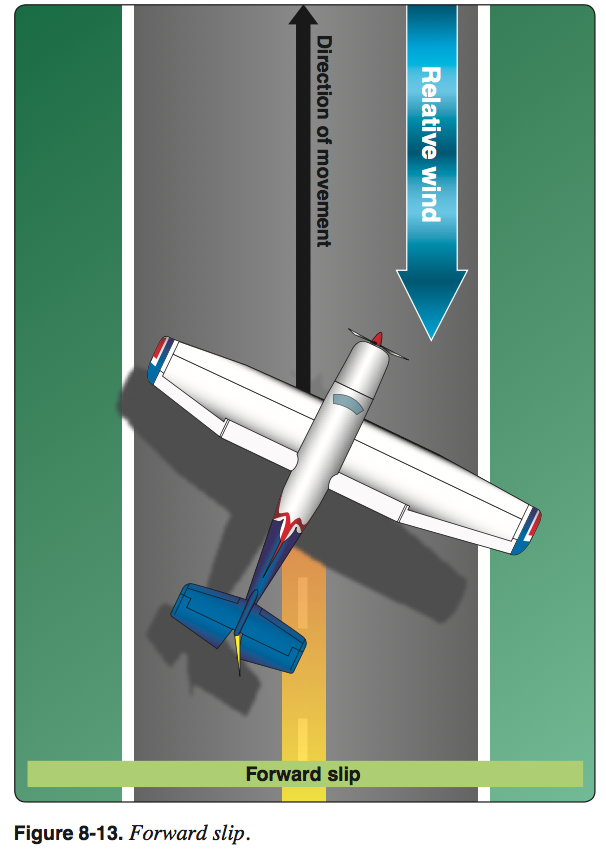
\includegraphics[width=\linewidth]{Forward Slip.png}
		\end{wrapfigure}

		A “forward slip” is one in which the airplane’s direction of motion continues the same as before the slip was begun. The wing on the side toward which the slip is to be made should be lowered by use of the ailerons. Simultaneously, the airplane’s nose must be yawed in the opposite direction by applying opposite rudder so that the airplane’s longitudinal axis is at an angle to its original flightpath. In a forward slip, the amount of slip, and therefore the sink rate, is determined by the bank angle. The steeper the bank is, the steeper the descent. Discontinuing a slip is accomplished by leveling the wings and simultaneously releasing the rudder pressure while readjusting the pitch attitude to the normal glide attitude. Because of the location of the pitot tube and static vents, airspeed indicators in some airplanes may have considerable error when the airplane is in a slip.The pilot must be aware of this possibility and recognize a properly performed slip by the attitude of the airplane, the sound of the airflow, and the feel of the flight controls.  Fuel indications become unreliable as fuel sloshes in the wing tanks. Unlike skids, however, if an airplane in a slip is made to stall, it displays very little of the yawing tendency that causes a skidding stall to develop into a spin. \footnote{\href[page=147]{./afh.pdf}{AFH - Intentional Slips}} \\

		ACS Requirements for a Forward Slip to a Landing\footnote{\href[page=39]{./private_airplane_acs.pdf}{ACS - Forward Slip to a Landing (ASEL, ASES)}}:
		\begin{enumerate}
			\item Complete the appropriate checklist. 
			\item Make radio calls as appropriate.
			\item Plan and follow a flightpath to the selected landing area considering altitude, wind, terrain, and obstructions.
			\item Select the most suitable touchdown point based on wind, landing surface, obstructions, and airplane limitations.
			\item Position airplane on downwind leg, parallel to landing runway
			\item Configure the airplane correctly
			\item As necessary, correlate crosswind with direction of forward slip and transition to side slop before touchdown.
			\item Maintain a ground track aligned with the runway center/landing path.
		\end{enumerate}

	\subsection{Go-Around}
		A go-around is a routine maneuver that should be executed anytime when an approach or landing in unsatisfactory. There are many factors that can contribute to unsatisfactory landing conditions. Situations such as air traffic control (ATC) requirements, unexpected appearance of hazards on the runway, overtaking another airplane, wind shear, wake turbulence, mechanical failure, and/or an unstable approach are all examples of reasons to discontinue a landing approach and make another approach under more favorable conditions. \footnote{\href[page=148]{./afh.pdf}{AFH - Go-Arounds (Rejected Landings)}}\\

		To execute a go around; apply full power, incrementally retract flaps while establishing a climb and inform Tower or others on CTAF of the go-around.\\

		ACS Requirements for a Go-Around/Rejected Landing\footnote{\href[page=40]{./private_airplane_acs.pdf}{ACS - Go-Around/Rejected Landing}}
		\begin{enumerate}
			\item Complete the appropriate checklist.
			\item Make radio calls as appropriate
			\item Make a timely decision to discontinue the approach to landing
			\item Apply takeoff power immediately and transition to climb pitch attitude for $V_X$ or $V_Y$ as appropriate ${}^{+10}_{-5}$ knots.
			\item Configure the airplane after a positive rate of climb has been verified or in accordance with airplane manufacturer's instructions.
			\item Maneuver to the side of the runway/landing area when necessary to clear and avoid conflicting traffic.
			\item Maintain $V_Y {}^{+10}_{-5}$ knots to a safe maneuvering altitude.
			\item Maintain directional control and proper wind-drift correction throughout the climb.
		\end{enumerate}
%done
\newpage
\section{Manoeuvres}

	Before each maneuver one must complete a HACL checklist:
	\begin{itemize}
		\item \textbf{H}eight, at least 1500 ft AGL (2500 ft AGL, CAE) (\href{https://www.law.cornell.edu/cfr/text/14/91.303}{91.303 (e)}), for stalls and performance manoeuvres; 600-1000 AGL for ground reference manoeuvres.
		\item \textbf{A}rea, not above congested areas, open air assembly of persons, within the lateral boundaries of the surface areas of Class B,C,D,E airspace designated for an airport, or within 4 nmi of the centerline of any Federal airway, or when flight visibility is less than 3 mi. (\href{https://www.law.cornell.edu/cfr/text/14/91.303}{91.303 (a-d,f)})
		\item \textbf{C}ockpit secure; no large loose articles, seats and seatbelt secure, fuel pump on, engine indications within limits
		\item \textbf{L}ookout, clearing turns; either a 180 degree or two 90 degree turns.
	\end{itemize}

	\subsection{Slow Flight}
		Slow flight is condition where flight is maintained at an attitude such that any increase in angle of attack would cause a stall indication, either a stall horn, or an approach to a buffet. In this condition, pitch is primarily used to control airspeed and power is used to control altitude. This condition is known as the \textbf{region of revered command}. In a slow flight attitude, induced drag is very high, and power must be applied to maintain airspeed and altitude. Turns during slow flight will require larger control inputs, as the decreased airspeed during slow flight decreases the effectiveness of the ailerons. Slow flight best replicates manuoeuvering an aircraft during landing.\\

		ACS Requirements for Slow Flight: \footnote{\href[page=47]{./private_airplane_acs.pdf}{ACS requirements for slow flight}}:
		\begin{enumerate}
			\item Clear the area, at an altitude no lower than 1500 ft AGL.
			\item Establish and maintain an airspeed at which any further increase in angle of attack, increase in load factor, or reduction in power, would result in a stall warning (e.g., airplane buffet, stall horn, etc.).
			\item Accomplish coordinated straight-and-level flight, turns, climbs, and descents with the airplane configured as specified by the evaluator without a stall warning (e.g., airplane buffet, stall horn, etc.).
			\item Maintain the specified altitude $\pm 100$ feet; specified heading $\pm 10^\circ$; airspeed ${}^{+10}_{-0}$ knots; and specified angle of bank $\pm 10^\circ$
		\end{enumerate}

	\subsection{Stalls}
		A stall is the aerodynamic condition when the wings fail to produce enough lift to overcome the force of gravity. All stalls are the result of the airplane exceeding the critical angle of attack for a given configuration. A stall can be identified by aural warnings such as a stall warning horn, a negative vertical speed indication at a positive attitude, or an aerodynamic buffet as airflow detaches from the wings.\\

		All stalls can be recovered from with these basic steps:
		\begin{enumerate}
			\item Pitch down, or simply relieve back pressure
			\item Increase power, noting P-factor will tend to turn the aircraft to the left.
			\item Slowly pitch up to recover, avoiding a secondary stall.
		\end{enumerate}

		A secondary stall occurs when the critical angle of attack is exceeded during the recovery, due to the increased load factor that can occur when pitching up too abruptly.

		\subsubsection{Power-Off Stall}
		\paragraph{(Clean)}
		A clean power-off stall is entered by reducing power to idle, and pitching to maintain altitude. It replicates the scenario that can occur during an engine failure, when a pilot fails to maintain best glide speed, and instead pitches to maintain altitude and inadvertently stalls instead.

		\paragraph{(Landing)} A power-off stall in the landing configuration simulates the stall that may inadvertently occur when landing; when a pilot may reduce power to idle and pitch up too early. To recover from a landing stall, retract flaps to take/off, apply full power and pitch down until sufficient airspeed is attained, and progressively pitch up.\\

		ACS requirements for power-off stalls: \footnote{\href[page=48]{./private_airplane_acs.pdf}{ACS requirements for power-off stalls}}:
		\begin{enumerate}
			\item Clear the area and select an entry altitude that will allow the task to be completed no lower than 1,500 feet AGL.
			\item Configure the airplane in the approach or landing configuration, as specified by the evaluator, and maintain coordinated flight throughout the maneuver.
			\item Establish a stabilized descent, and transition from the approach/landing attitude to induce a stall.
			\item Maintain a specified heading $\pm10^\circ$ if in straight flight; maintain a specified angle of bank not to exceed $20^\circ$, $\pm 10^\circ$ if in turning flight, while inducing the stall.
			\item Acknowledge cues of the impending stall and then recover promptly after a full stall occurs.
			\item Execute a stall recovery in accordance with procedures set forth in the POH/AFM.
			\item Configure the airplane as recommended by the manufacturer, and accelerate to $V_X$ or $V_Y$.
			\item Return to the altitude, heading, and airspeed specified by the evaluator. 
		\end{enumerate}

		\subsubsection{Power-On Stall (Takeoff Stall, Clean)}

		A power-on stall simulates the stall that may occur while taking off, at a high power setting and excessive pitch-up attitude. A power-on stall is usually accompannied by a strong left turning tendancy, due to the high power setting and low airspeed.\\

		ACS Requirements for power-on stalls: \footnote{\href[page=49]{./private_airplane_acs.pdf}{ACS requirements for power-on stalls}}
		\begin{enumerate}
			\item Clear the area and select an entry altitude that will allow the Task to be completed no lower than 1,500 feet AGL.
			\item Set power (as assigned by the evaluator) to no less than 65 percent available power. 
			\item Transition smoothly from the takeoff or departure attitude to the pitch attitude that will induce a stall. 
			\item Maintain a specified heading $\pm10^\circ$ if in straight flight; maintain a specified angle of bank not to exceed $20^\circ$, $\pm 10^\circ$ if in turning flight, while inducing the stall.
			\item Acknowledge cues of the impending stall and then recover promptly after a full stall occurs.
			\item Execute a stall recovery in accordance with procedures set forth in the POH/AFM.
			\item Configure the airplane as recommended by the manufacturer, and accelerate to $V_X$ or $V_Y$.
			\item Return to the altitude, heading, and airspeed specified by the evaluator. 
		\end{enumerate}

		\subsubsection{Spin Awareness}

		Although spins are not tested in the Private Pilot ACS, one must still demonstrate knowledge of how spins occur and the proper recovery technique. Spins occur when a wing is more stalled than the other, creating a yawing moment that induces a spin. Spin recovery is given by the PARE checklist:
		\begin{itemize}
			\item \textbf{P}ower to idle
			\item \textbf{A}ilerons neutral
			\item \textbf{R}udder opposite direction of rotation
			\item \textbf{E}levator down
		\end{itemize}

		As the spin is stopped, rudder neutral, slowly pitch up while increasing power, taking care to avoid a load factor induced stall.

	\subsection{Performance Manoeuvres}
		\subsubsection{Steep Turns}
			A steep turn is turn of $45^\circ$ bank for the Private Pilot ACS. A steep turn is a high performance turn, demonstrating a pilot's ability to turn in a relatively confined space while remaining coordinated, below manoeuvring speed. It is helpful to refer to the attitude indicator first to establish a $45^\circ$ bank, then to look outside to maintain a constant sight picture to maintain that bank.\\

			In a steep turn, one must compensate for the increased load factor by applying increased back pressure to maintain altitude. The increased AoA means that increased power is required to compensate for increased drag, As the steep turn is established, the wing on the outside of the turn rotates faster and generates more lift than the inner wing, so opposite aileron may be required to compensate for the overbanking tendency. Some rudder is required to remain coordinated, as left turning tendencies and adverse yaw affect the airplane's yaw during the maneuver.\\

		ACS requirements for steep turns: \footnote{\href[page=41]{./private_airplane_acs.pdf}{ACS requirements for steep turns}}
		\begin{enumerate}
			\item Clear the area and select an entry altitude that will allow the Task to be completed no lower than 1,500 feet AGL.
			\item Establish the manufacturer’s recommended airspeed; or if one is not available, a safe airspeed not to exceed $V_A$
			\item Roll into a coordinated $360^\circ$ steep turn with approximately a $45^\circ$ bank.
			\item Maintain the specified altitude $\pm 100$ feet;  airspeed $\pm 10$ knots; bank $\pm 5^\circ$, and roll out on the entry heading $\pm 10^\circ$
		\end{enumerate}			

	\subsection{Ground Reference}
		The purpose of ground reference maneuvers is to train pilots to accurately place the airplane in relationship to specific references and maintain a desired ground track. Such precision requires that a pilot simultaneously evaluate the airplane’s attitude, reference points along the desired path, and the natural horizon. To be effective, the pilot must scan between several visual references to determine relative motion and to determine if the airplane is maintaining, or drifting to or from, the desired ground track. Wind direction and velocity variations are the primary effects requiring corrections of the flightpath during ground reference maneuvers.\footnote{\href[page=114]{./afh.pdf}{(AFH Chapter 6: Ground Reference)}}\\

		Ground reference maneuvers are generally flown at altitudes between 600 and 1,000 feet above ground level (AGL). The pilot must consider the following when selecting the maneuvering altitude:
		\begin{itemize}
			\item The altitude should provide obstruction clearance of no less than 500 feet vertically above the obstruction and 2,000 feet horizontally.
			\item In case of an engine failure, the pilot must plan, consider, and be alert for forced landing areas while understanding that the lower the airplane’s altitude, the less time there is to configure the airplane for an emergency landing and the shorter the glide distance.
			\item Higher ground speed requires steeper banks and slower ground speed requires shallower banks. 
		\end{itemize}

		 All ground reference maneuvers should be entered on the downwind, noting that a steeper angle of bank will be required when turning with a higher ground speed, and a shallower angle of bank when turning at a lower ground speed. Steeper angles of attack will also be required when turning from the downwind side due to the wind pushing the aircraft outside the turn, conversely shallower angles of attack when turning with a headwind as the wind pushes the aircraft into the turn.

		\subsubsection{S-Turns}
			The S-turn is a ground reference maneuver that resembles drawing two half circles on opposite sides of a straight-line reference, easiest done along a road.

			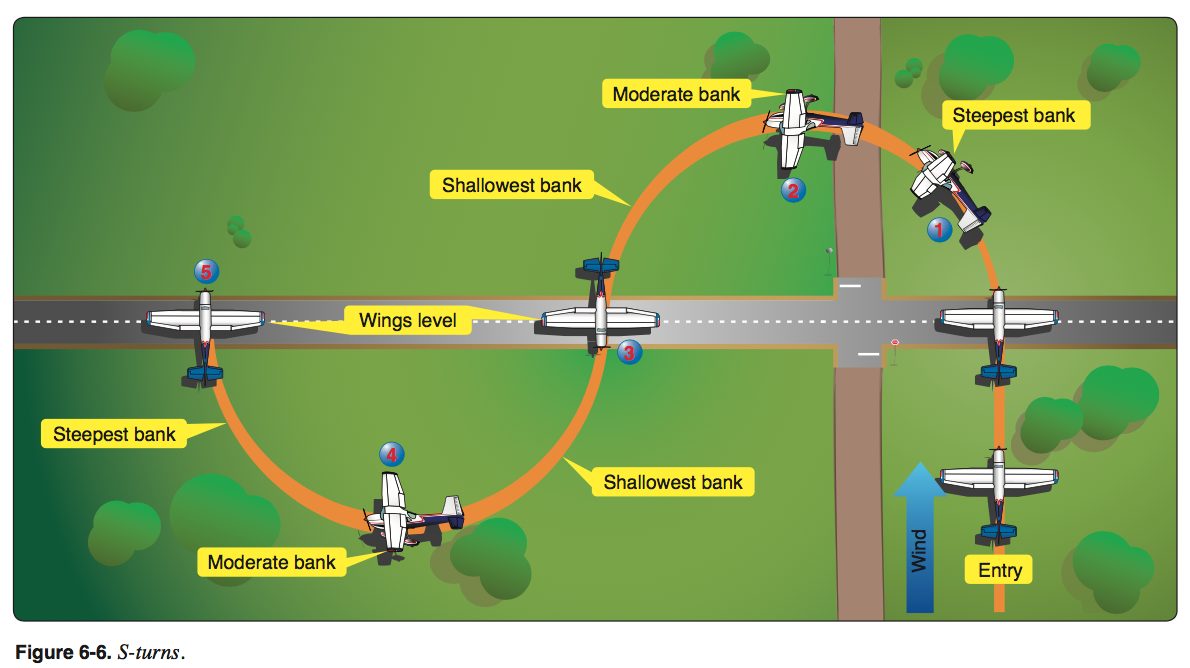
\includegraphics[width=\textwidth]{S-turns.png}

			ACS requirements for S-turns:\footnote{\href[page=42]{./private_airplane_acs.pdf}{ACS requirements for S-turns}}
			\begin{enumerate}
				\item Clear the area and select an entry altitude that will allow the task to be completed between 600 and 1000 feet AGL.
				\item Select a suitable ground reference line.
				\item Enter perpendicular to the selected reference line, 600 to 1,000 feet AGL at an appropriate distance from the selected reference area.
				\item Apply adequate wind-drift correction during straight and turning flight to maintain a constant radius turn on each side of a selected point. 
				\item Reverse the turn directly over the selected reference line. 
				\item Divide attention between airplane control, traffic avoidance and the ground track while maintaining coordinated flight. 
				\item Maintain altitude $\pm 100$ feet; maintain airspeed $\pm 10$ knots.
			\end{enumerate}

		\subsubsection{Turn around a Point}
			The turn around a point is a maneuver that is a $360^\circ$ constant radius turn around a single ground based reference point. It is easiest to select a compact, vertical, prominent structure to perform a turn around a point.

			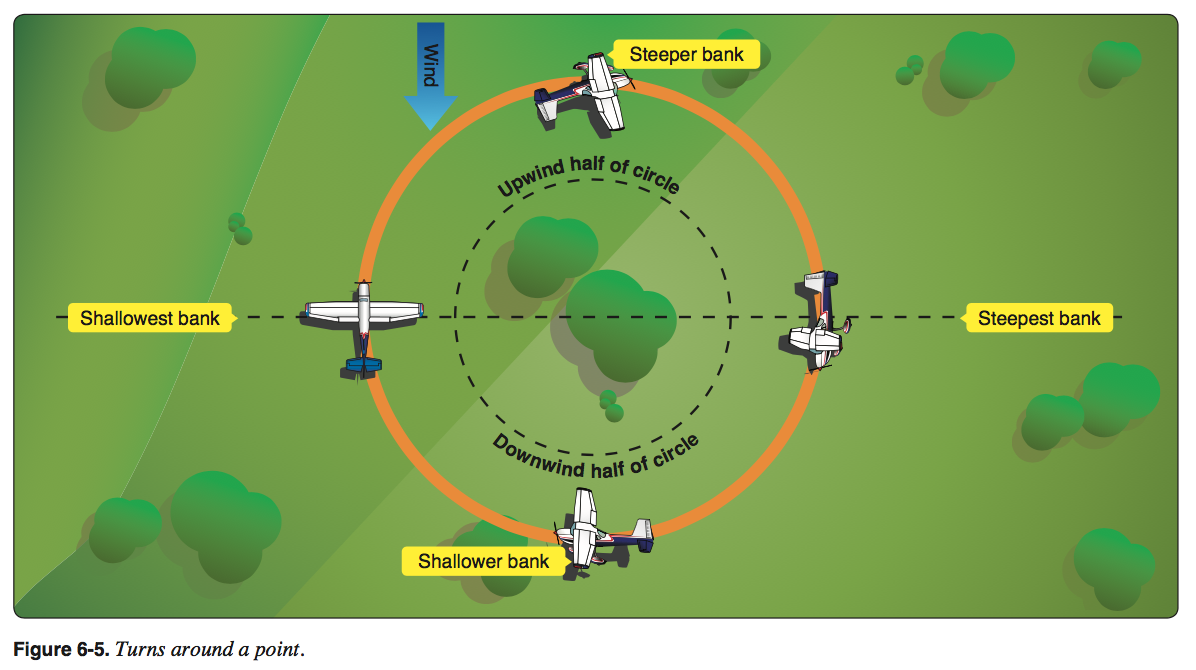
\includegraphics[width=\textwidth]{Turns around a point.png}

			ACS requirements for a turn around a point:\footnote{\href[page=42]{./private_airplane_acs.pdf}{ACS requirements for a turn around a point}}:
			\begin{enumerate}
				\item Clear the area and select an entry altitude that will allow the task to be completed between 600 and 1000 feet AGL.
				\item Select a suitable ground reference point as appropriate.
				\item Enter at an appropriate distance from the reference point, 600 to 1000 feet AGL at an appropriate distance from the selected reference area.
				\item Apply adequate wind-drift correction during straight and turning flight maintain a constant radius turn on each side of a selected reference point. 
				\item Divide attention between airplane control, traffic avoidance and the ground track while maintaining coordinated flight. 
				\item Maintain altitude $\pm 100$ feet; maintain airspeed $\pm 10$ knots.
			\end{enumerate}

		\subsubsection{Rectangular Course}
			The rectangular course is essentially a traffic pattern, executed at a constant altitude, airspeed, and distance from a ground reference. It is easiest to execute when selecting a ground reference that is approximately a rectangle.

			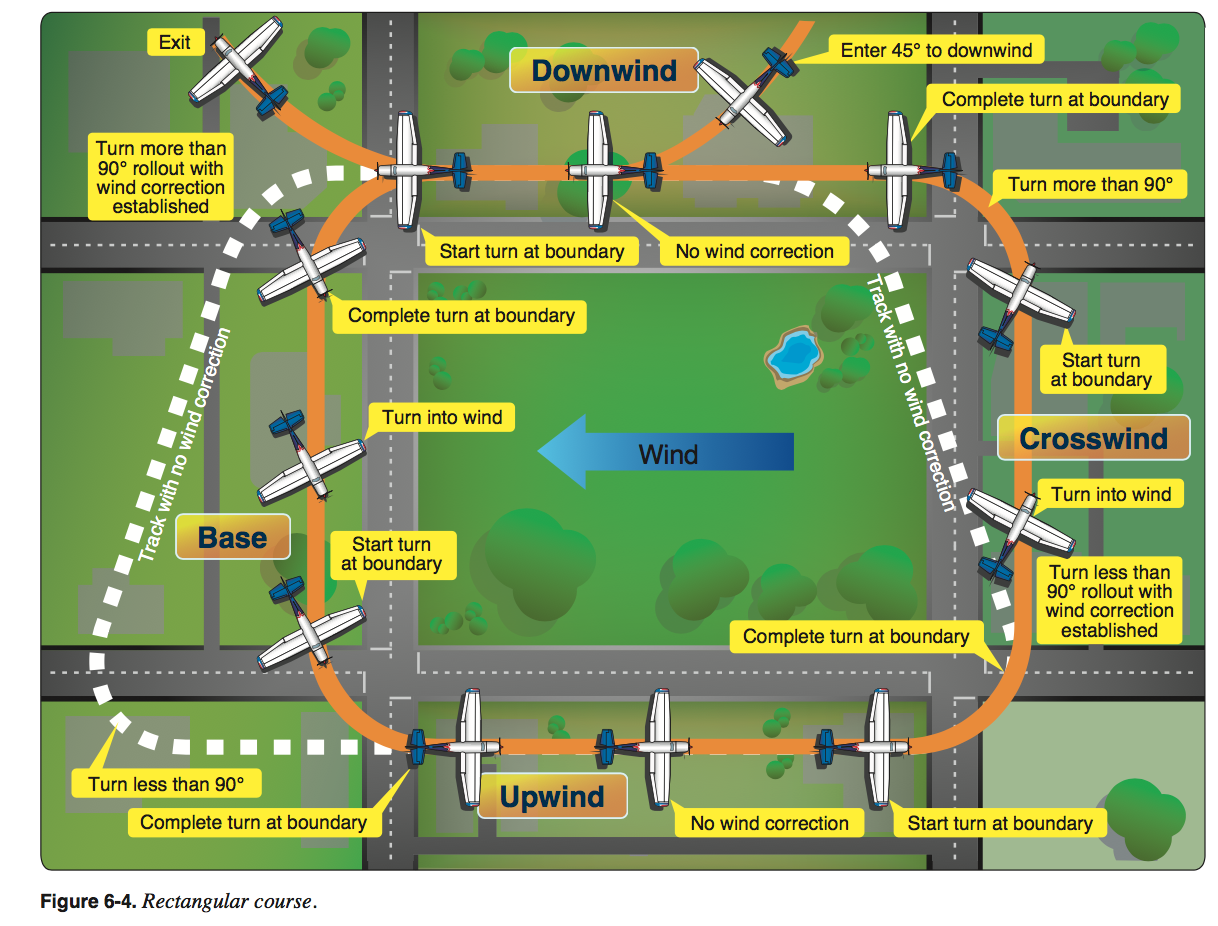
\includegraphics[width=\textwidth]{Rectangular course.png}

			ACS requirements for a rectangular course:\footnote{\href[page=42]{./private_airplane_acs.pdf}{ACS requirements for a rectangular course}}
			\begin{enumerate}
				\item Clear the area and select an entry altitude that will allow the task to be completed between 600 and 1000 feet AGL.
				\item Select a suitable ground reference point as appropriate.
				\item Enter a left or right pattern, 600 to 1,000 feet above ground level (AGL) at an appropriate distance from the selected reference area, $45^\circ$ to the downwind leg.
				\item Apply adequate wind-drift correction during straight and turning flight maintain a constant ground track around a rectangular reference area.
				\item Divide attention between airplane control, traffic avoidance and the ground track while maintaining coordinated flight. 
				\item Maintain altitude $\pm 100$ feet; maintain airspeed $\pm 10$ knots.
			\end{enumerate}

	\subsection{Instrument Maneuvers}
		Basic instrument maneuvers are taught to Private Pilot applicants in order to ensure their ability to maintain control of the airplane in the event of the loss of external visual reference, or spatial disorientation. It is important to trust one's instruments when inadvertently flying into IMC, and ignore sensory illusions that may occur when flying without external reference.\\

		Whenever finding oneself inadvertently in IMC, ATC is a valuable resource to use in order to safely navigate to a place where VFR flight can be resumed. ATC may assign turns and headings to VFR.

		\subsubsection{Straight \& Level Flight}
		 Straight and level flight is indicated by:
		 \begin{itemize}
		 	\item level attitude indicator
		 	\item constant altimeter reading
		 	\item constant compass/heading indication
		 	\item neutral turn \& skid indicator
		 	\item constant airspeed
		 \end{itemize}
		 ACS requirements for straight and level flight:\footnote{\href[page=51]{./private_airplane_acs.pdf}{ACS requirements for Straight \& Level Flight}}
		 \begin{enumerate}
		 	\item Maintain straight-and-level flight using proper instrument cross-check and interpretation, and coordinated control application.
		 	\item Maintain altitude $\pm 200$ feet, heading $\pm20^\circ$, airspeed $\pm 10$knots
		 \end{enumerate}
		\subsubsection{Climbs, Descents, \& Turns to Assigned Headings}
			To climb or descend, use the altimeter. In the case of a failed altimeter, but functional pitot ram-air source, you can use the airspeed indicator. In the absence of an all pitot-static instruments, you can use your attitude indicator. To turn to an assigned heading, simply use the HSI or heading indicator. In the absence of a HSI or heading instrument, use the magnetic compass.\\

			 ACS requirements for constant airspeed climbs \footnote{\href[page=52]{./private_airplane_acs.pdf}{Constant Airspeed Climbs}}, Constant Airspeed Descents\footnote{\href[page=53]{./private_airplane_acs.pdf}{Constant Airspeed Descents}},and turns to headings\footnote{\href[page=54]{./private_airplane_acs.pdf}{Turns to Headings}}:
		 \begin{enumerate}
		 	\item Maintain straight-and-level flight using proper instrument cross-check and interpretation, and coordinated control application.
		 	\item Maintain altitude $\pm 200$ feet, heading $\pm20^\circ$, airspeed $\pm 10$knots
		 \end{enumerate}

		\subsubsection{Unusual Attitudes}
			One may find oneself in an unusual attitude as a result of spatial disorientation, distractions, or upsets. There are two categories of unusual attitudes: nose high and nose low.\\

			Nose high attitudes are corrected by rolling wings level, increasing power, and pitching to a neutral attitude; taking care not to enter a power-on stall.\\

			 Nose low attitudes are corrected by rolling wings level, decreasing power, and pitching slowly up to a $0^\circ$ attitude; taking care to not exceed $V_{NE}$, or to exceed G-loading, or to stall.\\

			ACS requirements for recovery from unusual flight attitudes: \footnote{\href[page=55]{./private_airplane_acs.pdf}{ACS requirements for Recovery from Unusual Flight Attitudes}}
			 \begin{enumerate}
			 	\item Recognize unusual flight attitudes; perform the correct, coordinated, and smooth flight control application to resolve unusual pitch and bank attitudes while staying within the airplane’s limitations and flight parameters.
			 \end{enumerate}
\end{document}